% The Quantum Internet - A New Frontier
% Peter P. Rohde et al.

\def\pubmode{2}

% Publication mode:
%   0 = Draft without figures
%   1 = Dowling's eyes only
%   2 = Serious draft
%   3 = Arxiv (not serious, 2 column)
%	4 = Publisher (book)

% Specify configuration: (0 = off, 1 = on)
% 	sketchesmode 		= Sketches?
% 	seriousmode 		= Serious?
% 	maincontribstyle 	= Main/contributed or unified authorship list?
% 	QIPlink 			= Title page link to QIP project website?
% 	parainTOC 			= Paragraphs included in ToC?
% 	includelicense		= Creative Commons license page?
%	doublecol			= Two-column?

% Draft without figures
\if 0\pubmode
	\def\sketchesmode{0} 		% Sketches?
	\def\seriousmode{0} 			% Serious?
	\def\maincontribstyle{0} 	% Main/contributed or unified authorship list?
	\def\QIPlink{1} 			% Title page link to QIP project website?
	\def\parainTOC{0} 			% Paragraphs included in ToC?
	\def\includelicense{0}		% Creative Commons license page?
	\def\doublecol{1}

	\documentclass[draft, twocolumn, aps, rmp, amsmath, amssymb, nofootinbib, superscriptaddress, longbibliography, floatfix, table-of-contents, eqsecnum]{revtex4-2}
	\let\stdsection\section
	\renewcommand\section{\newpage\stdsection}
\fi

% Dowling's eyes only
\if 1\pubmode
	\def\sketchesmode{0} 		% Sketches?
	\def\seriousmode{1}	 		% Serious?
	\def\maincontribstyle{0} 	% Main/contributed or unified authorship list?
	\def\QIPlink{0} 			% Title page link to QIP project website?
	\def\parainTOC{0} 			% Paragraphs included in ToC?
	\def\includelicense{0}		% Creative Commons license page?
	\def\doublecol{0}

	\documentclass[preprint, aps, rmp, singlecolumn, amsmath, amssymb, nofootinbib, superscriptaddress, longbibliography, floatfix, table-of-contents, eqsecnum]{revtex4-2}
\fi

% Serious draft
\if 2\pubmode
	\def\sketchesmode{0} 		% Sketches?
	\def\seriousmode{1} 			% Serious?
	\def\maincontribstyle{0} 	% Main/contributed or unified authorship list?
	\def\QIPlink{0} 			% Title page link to QIP project website?
	\def\parainTOC{0} 			% Paragraphs included in ToC?
	\def\includelicense{0}		% Creative Commons license page?
	\def\doublecol{0}

	\documentclass[singlecolumn, aps, rmp, amsmath, amssymb, nofootinbib, superscriptaddress, longbibliography, floatfix, table-of-contents, eqsecnum]{revtex4-2}
	\pagestyle{empty}
\fi

% Arxiv
\if 3\pubmode
	\def\sketchesmode{1} 		% Sketches?
	\def\seriousmode{0} 			% Serious?
	\def\maincontribstyle{0} 	% Main/contributed or unified authorship list?
	\def\QIPlink{1} 			% Title page link to QIP project website?
	\def\parainTOC{0} 			% Paragraphs included in ToC?
	\def\includelicense{1}		% Creative Commons license page?
	\def\doublecol{1}

	\documentclass[twocolumn, aps, rmp, amsmath, amssymb, nofootinbib, superscriptaddress, longbibliography, floatfix, table-of-contents, eqsecnum]{revtex4-2}
\fi

% Publisher
\if 4\pubmode
	\def\sketchesmode{1} 		% Sketches?
	\def\seriousmode{0} 			% Serious?
	\def\maincontribstyle{1} 	% Main/contributed or unified authorship list?
	\def\QIPlink{0} 			% Title page link to QIP project website?
	\def\parainTOC{0} 			% Paragraphs included in ToC?
	\def\includelicense{0}		% Creative Commons license page?
	\def\doublecol{0}

	\documentclass[singlecolumn, aps, rmp, amsmath, amssymb, nofootinbib, superscriptaddress, longbibliography, floatfix, table-of-contents, eqsecnum]{revtex4-2}
	\let\stdpart\part
	\renewcommand\part{\newpage\stdpart}
\fi

\usepackage[pdftex]{graphicx}
\usepackage[dvipsnames]{xcolor}
\usepackage{mathrsfs}
\usepackage[colorlinks,breaklinks]{hyperref}
\usepackage{url}
\usepackage{makeidx}
\usepackage{nomencl}
\usepackage{colortbl}
\usepackage[section]{placeins}
\usepackage{qcircuit}
\usepackage{array}
\usepackage{amsmath}
\usepackage[noend]{algpseudocode}
\usepackage{mdframed}
\usepackage{type1cm}
\usepackage{lettrine}
\usepackage{dblfloatfix}
\usepackage{afterpage}
\usepackage[section]{placeins}
\usepackage[english]{babel}
\usepackage{lmodern}
\newcommand{\bra}[1]{\langle#1|}
\newcommand{\ket}[1]{|#1\rangle}

\newcommand\gobbleone[1]{}
\newcommand*{\seeonly}[2]{\ (\textit{\seename} #1)}
\newcommand*{\also}[2]{(\textit{\alsoname} #1)}

\newcommand{\smallaffiliation}[1]{\affiliation{\small #1}}
\newcommand{\boldauthor}[1]{\author{\textbf{#1}}}

\newcommand{\comment}[1]{{\color{blue}{\textbf{#1}}}}
\newcommand{\sihui}[1]{{\color{Orchid}{#1}}}

\newcommand{\latinquote}[1]{\textit{--- #1}\index{Latin}}

\newcommand{\dropcap}[2]{\lettrine[lines=2, findent=3pt, nindent=0pt]{#1}{#2}}
%\newcommand{\dropcap}[2]{#1#2}

\newcounter{regtablecntr}
\setcounter{regtablecntr}{0}
\newcounter{algcntr}
\setcounter{algcntr}{0}

\newcommand{\startnormtable}{
	\renewcommand{\tablename}{TABLE.}
	\setcounter{algcntr}{\value{table}}
	\setcounter{table}{\value{regtablecntr}}
}

\newcommand{\startalgtable}{
	\renewcommand{\tablename}{ALG.}
	\setcounter{regtablecntr}{\value{table}}
	\setcounter{table}{\value{algcntr}}
}

\if 0\sketchesmode
	\newcommand{\sketch}[1]{}
\fi
\if 1\sketchesmode
	\newcommand{\sketch}[1]{\begin{center}\includegraphics[width=0.4\textwidth]{#1}\end{center}\index{Artwork}}
\fi

\renewcommand{\tablename}{ALG.}
\renewcommand{\nomname}{List of Abbreviations}

%\newtheorem{definition}{Definition}
\newmdtheoremenv[innertopmargin=3pt, innerbottommargin=3pt, nobreak]{definition}{Def}
%\newtheorem{postulate}{Postulate}
\newmdtheoremenv[innertopmargin=3pt, innerbottommargin=3pt, nobreak]{postulate}{Post}

\makeatletter
\def\BState{\State\hskip-\ALG@thistlm}
\makeatother

\graphicspath{{./Figures/}}

\hypersetup{
	pdfauthor = {Peter P. Rohde},
	pdftitle = {The Quantum Internet},
	pdfsubject = {Quantum Internet},
	pdfkeywords = {Quantum, Computing, Information, Networks, Internet, Cryptography}
}

\makenomenclature
\makeindex

\begin{document}

%
% Entanglement distribution
%

\part{Entanglement distribution}\label{part:ent_dist}\index{Entanglement!Distribution}

%
% Entanglement - The Ultimate Quantum Resource
%

\section{Entanglement -- The ultimate quantum resource} \label{sec:ent_ultimate} \index{Entanglement}

As we have seen, the diversity of quantum states that may be communicated, and protocols implemented over the quantum internet is extremely diverse, encompassing many different types of encodings and communications protocols.

Given this plethora of protocols, discussed in detail in Sec.~\ref{sec:protocols_quant_int}, one might ask whether there is a single primitive resource that might be applicable to all, or at least most of these quantum protocols, thereby reducing the technological requirements of the nodes and quantum channels forming the network.

It turns out that there is one particularly useful quantum resource, that finds applicability in many of these protocols -- entanglement, specifically in the form of Bell-pairs (Sec.~\ref{sec:bell_state_res}).

In brief, Bell-pairs find applicability in, amongst many others, the following key protocols:
\begin{itemize}
\item Cluster states (Sec.~\ref{sec:CSQC}): a Bell-pair is also a two-qubit cluster state, a supply of which can be employed in fusion strategies to prepare larger cluster states, enabling universal MBQC.
\item Quantum state teleportation (Sec.~\ref{sec:teleport}): a shared Bell-pair between Alice and Bob forms the elementary quantum resource upon which the state teleportation protocol is constructed.
\item Quantum gate teleportation (Sec.~\ref{sec:teleport_gate}): a shared 4-qubit entangled state allows the teleportation of a CNOT gate. This 4-qubit state may be prepared from a resource of two Bell-pairs.
\item QKD (Sec.~\ref{sec:QKD}): the E91 protocol is built upon a reliable stream of distributed Bell-pairs.
\item Modularised quantum computation (Sec.~\ref{sec:module}): using Bell-pairs, entanglement swapping (Sec.~\ref{sec:swapping}) can be employed to fuse neighbouring, but potentially distant modules together using operations local to each module.
\item Superdense coding (Sec.~\ref{sec:superdense}): a shared Bell-pair enables the communication of two classical bits of information via a single qubit, thereby doubling classical channel capacity.
\end{itemize}

Thus, we see that Bell-pairs form a ubiquitous resource, covering many of the most significant quantum protocols -- quantum computation, distributed quantum computation, quantum state and gate teleportation, and quantum cryptography. This warrants special treatment of entanglement distribution, as a fundamental building block in the quantum era.

One might envisage a quantum internet in which a central server, who specialises in only Bell state preparation and distribution, serves the sole role of pumping out Bell-pairs across the internet to whomever requests them, who subsequently use them for protocols such as those mentioned above. This could be in the form of a server transmitting over fibre networks, across free-space, or via a satellite in orbit, transmitting at an intercontinental level.

What's the advantage of this approach to quantum networking? There are several:
\begin{itemize}
\item Dedicated servers can specialise in this one particular task, as can be the transmission infrastructure. The server needn't concern itself with the nitty-gritty of the protocols implemented by the end-user.
\item Because servers are providing a single standardised product, they can be commodified, enabling mass production of the hardware devices and the associated economy of scale.
\item Unlike generic quantum states, Bell-pairs are known states that can be infinitely reproduced, without having to worry about no-cloning limitations.
\item Photonic Bell-pairs are easily prepared via type-II SPDC at very high repetition rates (\mbox{$\sim 100$MHz-1GHz}), enabling rapid state preparation.
\item Bell-pairs are relatively `cheap' to prepare, and can be readily manufactured using widely accessible, present-day technology.
\item QoS is a lesser issue in most scenarios. We can employ a \textsc{Send-and-forget}\index{Send-and-forget strategy} protocol for the distribution of entanglement (much like classical UDP). Since every Bell-pair is identical, we needn't be concerned about missing ones. Instead, we can simply wait for the next one (a \textsc{Repeat-until-success}\index{Repeat-until-success strategy} strategy), knowing it will be exactly the same. We call this the \textsc{Shotgun}\index{Shotgun state preparation} approach -- keep firing away until we hit something.
\item Rather than transmitting quantum states between distant parties directly, if we instead use state teleportation, the state to be transmitted will not be corrupted if the communications channel fails (e.g via loss). Instead we can wait for the next successfully transmitted Bell-pair until we are ready to teleport the state, which then proceeds without directly utilising the quantum communications channel, accumulating its associated costs, or risking losing the state altogether should link failure occur. Only classical communication is required to complete the protocol, which can be regarded as error-free for all intents and purposes.
\item Entanglement purification may be employed by the two parties to improve the cost metrics associated with their shared entanglement, thereby partially overcoming the limitations imposed by the quantum communication channels.
\item If no direct link exists between server and clients, bootstrapped entanglement swapping can be employed to concatenate servers to create longer-distance `virtual' links. This is the basis for \textit{quantum repeater networks}, to be discussed next in Sec.~\ref{sec:rep_net}.
\end{itemize}

\comment{Any other advantages?}

In addition to entanglement distribution, entangling measurements, e.g Bell state projections (Sec.~\ref{sec:bell_proj}), may be used as a primitive for many protocols. This is effectively entangled state distribution in reverse, whereby two clients transmit states to a host, who performs a joint entangling measurement upon them. For example, in the modularised model for cluster state quantum computing, two adjacent but distant modules might transmit optical qubits to a satellite, which projects them into the Bell basis, thereby creating a link between the respective modules. This isn't as powerful as entangled state distribution, since it cannot be used for, for example, E91 QKD, but nonetheless remains a powerful primitive for many protocols.

These observations lead us to naturally conclude that a quantum network specialised to this one particular task -- entanglement distribution -- would already be immensely useful, and on its own enable many key applications, such as many of the ones presented here in Sec.~\ref{sec:protocols_quant_int}.

\comment{Latin quote}\index{Latin}


\latinquote{Credo in unum deum.}

%
% Quantum Repeater Networks
%

\section{Quantum repeater networks} \label{sec:rep_net} \index{Quantum repeater networks}

\textit{Quantum repeaters} are devices that allow entanglement to be shared between distant nodes, when no direct line of communication is available from a server to its two clients. This is achieved using a bootstrapped entanglement swapping protocol (Sec.~\ref{sec:swapping}). Most commonly, this entanglement is in the form of Bell-pairs, which, as discussed previously in Sec.~\ref{sec:ent_ultimate}, form a ubiquitous resource for many essential quantum protocols. The actual physical encoding of the entangled states may vary, but is most commonly in the form of polarisation-encoded single-photons or CV states.

\comment{To do by Bill Munro}

\latinquote{Acta non verba.}

%
% The Irrelevance of Latency
%

\section{The irrelevance of latency}\index{Latency}

Entanglement distribution\index{Entanglement distribution} can be executed in a highly varying manner of ways -- from transmitting optical qubits through space via satellites, to across land surfaces via optical fibre, to dumping solid-state qubits into cargo containers and shipping them via land or sea freight. These bring with them associated transmission latencies. The former two distribute entanglement at the speed of light with latencies on the order of microseconds, whereas the latter induces enormous latencies on the order of days or weeks.

At first glance it may appear that this renders the Sneakernet\texttrademark\index{Sneakernet} approach to entanglement distribution useless. Who wants to wait several weeks to communicate their qubits?

If these transmission methods were being utilised for direct transmission of quantum data, this would certainly be a major concern. However, we are not employing them to communicate unknown quantum data packets directly. Rather we are using them to distribute many instances of completely identical Bell states. This changes the impact of latency entirely.

If our goal is to transmit a quantum state between two parties, the obvious approach is to send the qubits directly over the quantum channel. Alternately, they could initially share Bell-pairs then employ quantum state teleportation\index{Quantum state teleportation} to teleport the state between parties. In this case all that matters is that they hold a shared Bell-pair in time for execution of the teleportation protocol. It could have been distributed between them at any point in the past, held in a quantum memory\index{Quantum memory} until needed. The latency is now determined entirely by the latency of the \textit{classical} channel, which communicates the associated local corrections required to complete the teleportation protocol. In most classical networks, communication rates are on the order of the speed of light, with very little latency.

We see that the latency associated with entanglement distribution does not affect the latency of quantum state transmission when implemented via teleportation. The quantum network could continually be sharing entangled pairs between parties in a UDP-like\index{User datagram protocol} mode, who hold them in quantum memory. They ensure that Bell-pairs are being distributed at a sufficient rate that parties have a buffer of entangled pairs sufficient to accommodate demand for future teleportations. This irrelevance of quantum latency is a uniquely quantum phenomena, not applicable to any classical protocols.

Teleportation-based quantum communication is additionally favourable in that shared Bell-pairs can be purified before being utilised, allowing errors accrued during quantum communication to be minimised, something not so straightforward when transmitting data qubits directly.

\latinquote{Ceterum censeo carthaginem delendam esse.}

%%
% The Quantum Sneakernet
%

\section{The quantum Sneakernet\texttrademark}\index{Sneakernet}

\comment{To do. Simon Devitt.}

\begin{figure}[!htbp]
\if 3\pubmode
\includegraphics[width=0.7\textwidth]{sneakernet_boat}
\else
\includegraphics[width=0.475\textwidth]{sneakernet_boat}
\fi
\caption{\comment{To do}}\label{fig:sneakernet_boat}	
\end{figure}


\latinquote{Veritas vos liberabit.}

\sketch{sketch_7}

%
% Quantum cryptography
%

\part{Quantum cryptography}\label{part:quant_crypto}\index{Quantum cryptography}

%
% CryptoWars (TM)
%

\section{Quantum cryptography}\index{Quantum key distribution}\label{sec:cryptowars}

\comment{To do, AES, DES, RSA}

\comment{Add more advanced protocols? Decoy states, untrusted devices etc. etc.}

\comment{Index}

Undoubtedly, quantum technologies will be most impactful (and disruptive) in the area of information security, something of fundamental importance to us all on a daily basis. Quantum technologies will be important both in terms of breaking and maintaining security, with the former mandating interest in the latter.

In Sec.~\ref{sec:homo_blind} we discussed encrypted outsourced quantum computation as an important concept in future cloud quantum computing. In this section we will step back from full-fledged distributed quantum computation, instead focussing on more elementary protocols for simple secure communication.

Today, the ability to communicate secretly with others is completely taken for granted in all but a few nations and resides in every smartphone and desktop PC. Furthermore, the encryption technologies available to the average consumer are extremely strong, the same as those used by large organisations, including world governments.

\subsection{Classical cryptography}\index{Classical cryptography}

\subsubsection{Private-key cryptography}\index{Private-key cryptography}

Private- (or symmetric-) key cryptography is perhaps the most basic (and useful) cryptographic primitive, enabling encryption of a channel between two parties who share a secret key. The same secret key is employed for both encryption and decryption operations, making it of utmost importance that it be retained secret.

Private key cryptography has a long history, in fact going back to ancient times, enabling the secret sharing of diplomatic messages between emperors and empires. However it was a niche technology that very few utilised, since it had to be implemented by hand without computers.

Today there are countless freely available private-key cryptographic protocols available online, and some have been standardised by standards institutes. Currently, the Advanced Encryption Standard (AES) is a standard endorsed by the US government. AES is a block cipher, meaning that it divides data into small blocks of bits, each of which are encrypted independently, and operates with key lengths of up to 256 bits, making it very robust against brute-force attacks (Sec.~\ref{sec:brute_force_attack}).

%
% One-Time Pad Cipher
%

\subsubsection{One-time pad cipher}\index{One-time pad cipher}

There is only a single provably secure encryption protocol -- the \textit{one-time pad}\index{One-time pad cipher} \cite{bib:Schneier96}. This protocol requires Alice and Bob to share a random bit-string as long as the message (plaintext\index{Plaintext}) being communicated between them. The two bit-strings undergo bit-wise XOR operations to form the ciphertext\index{Ciphertext}. Mathematically,\index{One-time pad cipher}
\begin{align}
c = s \oplus k,
\end{align}
where $\oplus$ is the bitwise XOR operation (equivalently addition modulo 2), and $c$, $s$ and $k$ are the ciphertext, plaintext and key strings respectively, all of which are of the same length, \mbox{$|c|=|s|=|k|$}.

The security of this protocol is easy to see intuitively -- with an appropriate choice of key, \textit{any} plaintext of the same length could be inferred from the ciphertext. This means that there is no possibility of performing any kind of frequency analysis, as the ciphertext string has maximum entropy\index{Entropy} (inherited from the maximum entropy of the key, and assuming a strong cryptographic random bit generator) and thus no correlations. Alternately, suppose we were to try and crack this code by expressing the decryption as an oracle, where the input is a key bit-string. Then we use brute-force\index{Brute force} (or Grover's algorithm\index{Grover's algorithm}) to query the oracle for tagged elements, where by `tagged' we mean that it satisfies an appropriate test (e.g an English language test) to decide whether a decrypted message is valid. Since every possible valid plaintext can be recovered using an appropriate key, the protocol is unable to find a unique plaintext matching the ciphertext.

Importantly, the secrecy of the one-time-pad\index{One-time pad cipher} strictly requires that a key never be reused. A fresh key must be generated for each message sent, otherwise trivial frequency analysis\index{Frequency analysis} techniques can be employed to compromise security. If the same key $k$ is used to encode two messages $s_1$ and $s_2$, yielding ciphertexts,
\begin{align}
c_1&=s_1\oplus k,\nonumber\\
c_2&=s_2\oplus k,
\end{align}
then we trivially obtain,
\begin{align}
c_1 \oplus c_2 = s_1 \oplus k \oplus s_2 \oplus k = s_1 \oplus s_2.
\end{align}
Now a frequency analysis on the bitwise XOR of two plaintexts can be applied, without requiring any knowledge of the key whatsoever.

Needless to say, the requirement for keys of the same length as the plaintexts, which cannot be reused, raises the obvious criticism that now secret key-sharing is as difficult as sharing a secret message in the first place. This reduces the problem of perfect secrecy of arbitrary messages to the secrecy of shared randomness. 

\subsubsection{Public-key cryptography}\index{Public-key cryptography}

While private-key cryptography solves the problem of end-to-end cryptography, it has one main downfall -- how does one share a private key between two parties? After all, if we had the ability to secretly share keys between ourselves, wouldn't we just use that method to directly communicate, bypassing the unnecessary cryptographic protocol.

Public- (or asymmetric-) key cryptography addresses this issue by replacing the private key with two keys, one used solely for \textit{encryption}, the other solely for \textit{decryption}. Then to send a message to a friend I can send him my encryption (public) key that he is only able to use for preparing an encrypted message for me. No security is required when sharing the public key since an eavesdropper can't use it for decryption. Finally, I am able to decrypt the message using my decryption (private) key, which I kept completely to myself and never shared with anyone.

RSA \cite{bib:RSA} was the first published public-key cryptographic protocol, and forms the backbone for most encryption used on the internet today. It achieves its security based on the belief that factorising large integers into constituent primes is a computationally hard problem -- a so-called `trapdoor function'\index{Trapdoor function}. The private key comprises two prime numbers, which are multiplied together to obtain the public key. It is clear that to obtain the private key from the public key would require solving the integer factorisation problem, which is presumed to be intractable.

Since RSA, numerous other public-key crypto-systems have been developed, based on different choices of trapdoor function. However, RSA remains the most widely used public-key cipher.

\subsection{Attacks on classical cryptography}

\subsubsection{Classical attacks}

\paragraph{Brute-force}\index{Brute-force}\label{sec:brute_force_attack}

The most obvious approach to cracking a crypto-system is to systematically try out all possible keys until we find one that correctly decodes the encrypted message. This is also the most na\"ive approach, and one which is computationally intractable for real-world key lengths. Specifically, for a key length of $k$ bits (\mbox{$k=256$} for AES), there are $2^k$ possible keys to try, and on average we will wait for $2^{k-1}$ trials before choosing the right one. Clearly an average waiting time of $2^{128}$ is not plausible!

\paragraph{Cryptanalysis}\index{Cryptanalysis}

\paragraph{Integer factorisation}

\subsubsection{Quantum attacks}

\paragraph{Brute-force}

A brute-force attack by a quantum computer does not offer us the exponential improvement attacker Eve might hope for. However, we can gain a quadratic improvement by cleverly exploiting Grover's search algorithm (Sec.~\ref{sec:quantum_algs}).

To do this, we treat the brute-force cracking algorithm as a satisfiability problem, similar to how Grover's is employed to enhance \textbf{NP}-complete problems. Specifically, our oracle implements the code's decryption operation, taking as input a qubit string representing the key. After decoding the message with the key, the oracle runs an appropriate test on the decrypted message to determine whether it is a legitimate decoded message. For example, it could run an English language test -- a message decoded incorrectly with the wrong key will appear very random and almost certainly won't pass such a test.

\comment{Note that when performing a brute-force attack against a private encryption key\index{Private-key encryption}, a quadratic speedup effectively halves the key length in terms of algorithmic runtime. Thus, in the quantum era private key lengths will need to be doubled.}

\paragraph{Integer factorisation}

\subsection{The end of classical cryptography?}

\subsection{Post-quantum classical cryptography}\index{Post-quantum classical cryptography}

One of the main reasons quantum computation has received so much interest from nation states is their ability to efficiently crack some cryptographic protocols, most notably RSA.

\comment{Mcelise, NP-hard problem}

\subsection{The Blockchain}\index{Blockchain}

%
% Quantum Cryptography
%

\subsection{Quantum cryptography}\index{Quantum cryptography}

%
% Quantum Key Distribution (QKD)
%

\subsubsection{Quantum key distribution (QKD)} \label{sec:QKD} \index{Quantum key distribution (QKD)}

Aside from quantum computing, a central use for quantum technologies is in cryptography \cite{bib:Gisin02}. The demand for secure cryptography is now extremely important in the context of electronic commerce and general security of information transmission in the internet age. Electronic currencies such as Bitcoin\index{Bitcoin} depend on cryptographic protocols in order to secure the value of assets, assign ownership certificates\index{Owner certificates}, and secure the currency against fraud. However such protocols are based upon the computational complexity of certain mathematical problems (\textit{computational security}\index{Computational security}), and are not fundamentally secure in the presence of limitless computational resources, or quantum computers. Therefore, using quantum mechanical protocols based on physical principles (\textit{information-theoretic security}\index{Information-theoretic security}) rather than computational limitations, are favourable in the sense of future-proofing security.

QKD protocols facilitate shared, secret randomness, where any intercept-resend attack\index{Intercept-resend attack} (or man-in-the-middle attack) may be detected, guaranteed by the laws of quantum physics (specifically the Heisenberg uncertainty principle\index{Heisenberg uncertainty principle} and no-cloning theorem\index{No-cloning theorem}).

Quantum key distribution (QKD) is a relatively mature technology with already several commercial systems being available off-the-shelf\footnote{\cite{??? example companies}}. The main drawback is thus the ability to perform long-distance transmission of photons. For these reasons, current QKD networks have been limited to relatively small distances, on the order of $\sim100$km, including in Austria, Switzerland, Japan, USA, and China \cite{bib:lo2014secure}. The longest distance QKD network that is currently planned is the Beijing to Shanghai QKD link spanning a distance of 2,000km. This involves 32 trusted nodes\index{Trusted nodes} to break the total distance into shorter segments to convert the quantum information to classical information.

Utilising space communications for the purpose of QKD has been discussed in several works \cite{bib:hughes2000quantum, bib:rarity2002ground, bib:pfennigbauer2003free, bib:aspelmeyer2003long, bib:armengol08}. As already demonstrated in space-based entanglement experiments \cite{bib:yin2017satellite, bib:ren2017ground, bib:liao2017satellite} far lower attenuation rates are possible than ground-only approaches. Since cryptography schemes such as BB84\index{BB84 protocol} do not require entanglement, these would appear to be the first widespread commercial application for quantum technologies.  

The ready realisability of space based QKD was already noted in a variety of configurations including ground-to-space\index{Ground-to-space communication} and space-to-ground\index{Space-to-ground communication} quantum communication \cite{bib:rarity2002ground, bib:aspelmeyer2003long}. In the context of security, the first long-distance experiments that are likely to be demonstrated will employ trusted nodes\index{Trusted nodes}. For example, after performing QKD between satellite\index{Satellites} and ground stations, a satellite could store the key for some time until another QKD can be performed to another ground station\index{Ground stations} using a one-time pad\index{One-time pad cipher} \cite{bib:liao2017satellite}. These types of experiments are planned to eventually perform intercontinental QKD\index{Intercontinental QKD} between China and Austria.  

%
% BB84 & E91 Protocols
%

\paragraph{BB84 \& E91 protocols}

The two original QKD protocols, known as the \textit{BB84} \cite{bib:BennetBrassard84}\index{BB84 protocol}, and \textit{E91} \cite{bib:Ekert91}\index{E91 protocol} protocols, are based on polarisation encoding in photons. BB84 requires only the transmission of a sequence of single photons, polarisation-encoded\index{Polarisation encoding} with random data. E91, on the other hand, requires a server that distributes entangled Bell-pairs between Alice and Bob. Since then, numerous other protocols for QKD have been proposed, for example, using CV (continuous variable) states\index{Continuous variable QKD}.

Suppose an eavesdropper, Eve, were to perform an intercept-resend\index{Intercept-resend attack} attack on the channel between Alice and Bob. At that stage in the protocol Alice had not yet announced her choice of bases, and Eve will not know the bases in which to measure states without randomly collapsing them onto values inconsistent with Alice's encoding. By sacrificing a some of their shared bits, via openly communicating them to one another for comparison, such an attack will be detected with asymptotically high security. Thus, Alice and Bob have great confidence that they have a shared, secret, random bit-string, which may subsequently be employed in a one-time-pad.

\begin{table}[!htb]
\fbox{\parbox{0.965\columnwidth}{\texttt{ 
function BB84():
\begin{enumerate}
\item Alice chooses a random bit, $0$ or $1$.
\item Alice randomly chooses a basis, $\hat{X}$ or $\hat{Z}$.
\item Depending on the choice of basis, she encodes her bit into the polarisation of a single photon as:
\begin{align}
\ket{0}_Z &\equiv \ket{H}, \nonumber \\
\ket{1}_Z &\equiv \ket{V},
\end{align}
or,
\begin{align}
\ket{0}_X &\equiv \frac{1}{\sqrt{2}}(\ket{H}+\ket{V}), \nonumber \\
\ket{1}_X &\equiv \frac{1}{\sqrt{2}}(\ket{H}-\ket{V}).
\end{align}
\item Encoding into the randomly chosen basis, she transmits the randomly chosen bit to Bob.
\item She does not announce the choice of bit or basis.
\item Bob measures the bit in a randomly chosen basis, $\hat{X}$ or $\hat{Z}$.
\item The above is repeated many times.
\item Upon receipt of all qubits, Alice (publicly) announces the basis used for encoding each bit sent.
\item Qubits where Bob measured in the opposite basis to which Alice encoded are discarded, as they will be decorrelated from Alice.
\item The remaining measurement outcomes are guaranteed to yield identical bits between Alice and Bob.
\item Remaining is roughly half as many bits as were sent, which are random, but guaranteed to be identical between Alice and Bob.
\item Alice and Bob sacrifice some of their bits by publicly communicating them to check for consistency. This rules out intercept-resend attacks.
\item Privacy amplification may be used to distill the partially compromised key into a shorter but more secret one.
\end{enumerate}}}}
\caption{BB84 QKD protocol using polarisation-encoded\index{Polarisation encoding} photons. Upon completion of the protocol, Alice and Bob share a random bit-string.\index{One-time pad cipher}}\label{alg:bb84}
\end{table}

E91 is slightly different. Here Alice and Bob share an entangled Bell-pair provided by a central authority. Then both Alice \textit{and} Bob measure their qubits in random bases. As with BB84, after measuring all qubits, they compare their choices of random bases. When they coincide, they have a shared bit. When they don't, they discard their result. From here the remainder of the protocol is the same as for BB84.

\comment{Explain E91 in detail}

\comment{What's the other QKD protocol? Include it}

Like BB84, E91 has no mode-matching\index{Mode-matching} or interferometric stability\index{Interferometric stability} requirements, and Alice and Bob both only require single-photon detection. Unlike BB84, however, E91 requires a central authority that is able to prepare entanglement on-demand as a resource.

Importantly, unlike classical cryptographic protocols, QKD makes no assumptions about the computational complexity of inverting encoding algorithms. The protocol is information theoretically secure\index{Information-theoretic security}, and therefore no physically realisable computer, even a quantum computer, can compromise it. Thus, usual cryptanalytic techniques, like linear and differential cryptanalysis \cite{bib:Schneier96}\index{Linear cryptanalysis}\index{Differential cryptanalysis}, or the ability to factor large numbers, that are employed to attack other encryption protocols, do not compromise QKD.

It is easy to see the utility of quantum networks in enabling commodity deployment of QKD -- users desire to communicate photons across long-range ad hoc networks, with low loss and dephasing. A global quantum internet would allow quantum cryptography to truly supersede classical cryptography, bypassing the vulnerabilities faced by classical cryptography in the era of quantum computing.

QKD has been widely experimentally demonstrated over long distances \cite{bib:Muller96}, and unlike quantum computing, QKD is at the stage of commercial viability, with several vendors offering off-the-shelf plug-and-play QKD systems. Thus, a quantum internet with low cost metrics would already find substantial utility with today's technology. Currently, great progress in being made in the implementation of QKD in fibre \cite{???}, over free space \cite{bib:Buttler00}, and even over intercontinental satellite uplinks \cite{JWP}. It seems extremely likely that some government agencies would be rolling out QKD systems \cite{bib:Secret}, especially in light of the paranoia surrounding quantum codebreaking.

In Sec.~\ref{sec:state_of_the_art} we summarise the state-of-the-art in the physical implementation of QKD.

%
% Quantum Anonymous Broadcasting
%

\subsubsection{Quantum anonymous broadcasting} \label{sec:anon_broad} \index{Quantum anonymous broadcasting}

\cite{Wehner}

\comment{Ryan TO DO}

\comment{Talk about Wehner scheme, as well as Brennen/Menicucci toric code scheme.}

\latinquote{A mari usque ad mare.}

\sketch{sketch_8}

%
% Quantum computing
%

\part{Quantum computing}\label{part:QC}\index{Quantum computing}

\dropcap{S}{ince} quantum computing is perhaps the most exciting of the emerging quantum technologies, which we treat as the foremost application for the quantum internet, we now introduce quantum computing, covering models and physical implementations for realising it, and some of its well-known algorithmic applications.

%
% Models For Quantum Computation
%

\section{Models for quantum computation} \label{sec:models_QC} \index{Models for quantum computation}

\dropcap{W}{e} begin by reviewing the models for quantum computation that we will refer to throughout this work.

There are various approaches to implementing and representing quantum computations. We now briefly introduce the ones most relevant to our discussions on networked quantum computation. Other formalisms, such as adiabatic quantum computation \cite{???} and quantum simulated annealing \cite{???}, which are not so obviously applicable to networking, will not be introduced, although many excellent introductions to these fields exist \cite{???}.

%
% Quantum Circuits
%

\subsection{Circuit model} \label{sec:circuit_model} \index{Circuit model}

The \textit{circuit model} is the conventional and most intuitive approach for expressing quantum algorithms, decomposing them into chronological sequences of elementary operations, comprising state preparation, single- and multi-qubit gates, measurement, and classical feedforward. We recommend referring to the introductory sections of \cite{bib:NielsenChuang00} for a far more comprehensive introduction to quantum circuits than is presented here. This model will be naturally intuitive to those familiar with classical circuit diagrams, albeit with some important differences, such as time-ordering.

\begin{figure}[!htbp]
	\begin{align}
		\Qcircuit @C=.7em @R=.4em @! {
		\lstick{\ket{\psi_1}} & \qw & \qw & \ctrl{1} & \gate{Y} & \meter & \control \cw\\
		\lstick{\ket{\psi_2}} & \qw & \targ & \ctrl{-1} & \qw & \meter & \cwx\\
		\lstick{\ket{\psi_3}} & \gate{H} & \ctrl{-1} & \qw & \qw & \gate{X} \cwx & \gate{Z} \cwx & \rstick{\ket{\phi}} \qw
		} \nonumber
	\end{align}
	\captionspacefig \caption{Simple example of a quantum circuit on 3 qubits, comprising several single- and 2-qubit quantum gates and measurements. Rows represent qubits, and time flows from left-to-right.} \label{fig:eg_circuit}
\end{figure}

Fig.~\ref{fig:eg_circuit} illustrates a simple 3-qubit quantum circuit comprising all of these elements. The interpretation of this diagram is as follows:
\begin{itemize}
	\item Horizontal lines represent individual qubits.
	\item Time flows from left to right (feedback is not allowed in the typical formalism for this representation).
	\item The three input qubits are labelled on the far-left as $\ket{\psi_1}$, $\ket{\psi_2}$ and $\ket{\psi_3}$.
	\item Single-qubit gates are denoted as boxes containing the name of the associated unitary operation. Here, the examples are the Hadamard ($\hat{H}$), Pauli bit-flip ($\hat{X}$), Pauli bit-phase-flip ($\hat{Y}$), and Pauli phase-flip ($\hat{Z}$) gates\index{Pauli operators}\index{Hadamard!Gate},
	\begin{align}
		\hat{H} &= \frac{1}{\sqrt{2}}\begin{pmatrix}
		1 & 1 \\
		1 & -1
		\end{pmatrix},\nonumber \\
		\hat{X} &= \begin{pmatrix}
		0 & 1 \\
		1 & 0
		\end{pmatrix},\nonumber \\
		\hat{Y} &= \begin{pmatrix}
		0 & -i \\
		i & 0
		\end{pmatrix},\nonumber \\
		\hat{Z} &= \begin{pmatrix}
		1 & 0 \\
		0 & -1
		\end{pmatrix}.
	\end{align}
	\item 2-qubit gates are denoted by vertical lines between the respective qubits.
	\item The maximally-entangling 2-qubit controlled-NOT (CNOT) gate\index{Controlled-NOT (CNOT) gates} is denoted via a control ($\bullet$) and a target ($\oplus$),
	\begin{align}
		\hat{\mathrm{CNOT}}=\begin{pmatrix}
		1 & 0 & 0 & 0 \\
		0 & 1 & 0 & 0 \\
		0 & 0 & 0 & 1 \\
		0 & 0 & 1 & 0
		\end{pmatrix}.
	\end{align}
	This is the quantum equivalent of the classical XOR gate, flipping the target ($\hat{X}$) if the control is on.
	\item All quantum gates have the same number of input as output qubits. This is a necessary condition for the unitarity of quantum gates (\mbox{$\hat{U}^\dag \hat{U} = \hat{\mathbb{I}}$}).
	\item The maximally-entangling 2-qubit controlled-phase (CZ)\index{Controlled-Z (CZ) gates} gate is denoted by two targets ($\bullet$) (the gate operates symmetrically on its two qubits),
	\begin{align}
		\hat{\mathrm{CZ}}=\begin{pmatrix}
		1 & 0 & 0 & 0 \\
		0 & 1 & 0 & 0 \\
		0 & 0 & 1 & 0 \\
		0 & 0 & 0 & -1
		\end{pmatrix},
	\end{align}
	applying a phase-gate ($\hat{Z}$) to the target if the control is on.
	\item The `meter' symbol represents a classical measurement in the Pauli $\hat{Z}$-basis (the computational or logical basis).
	\item Double lines represent classical feedforward of measurement outcomes, controlling a subsequent gate.
\end{itemize}

The circuit in Fig.~\ref{fig:eg_circuit} can be interpreted mathematically as implementing the following operation,
\begin{align}
	\ket\phi &= {\hat{Z}_3}^{m_1} \cdot {\hat{X}_3}^{m_2} \cdot \hat{M}_2 \cdot \hat{M}_1 \cdot \hat{Y}_1 \nonumber \\
	&\cdot \hat{\mathrm{CZ}}_{1,2} \cdot \hat{\mathrm{CNOT}}_{3,2} \cdot \hat{H}_3 \cdot \ket{\psi_1}\otimes\ket{\psi_2}\otimes\ket{\psi_3},
\end{align}
where $m_1$ and $m_2$ are the binary measurement outcomes of the two single-qubit $\hat{Z}$-basis measurements, $\hat{M}_1$ and $\hat{M}_2$.

Using the circuit model, arbitrary quantum computations can be elegantly and intuitively represented. To enable \textit{universal} quantum computation within this model, a \textit{universal gate set} must be available at our disposal. Most commonly, this is chosen to be the maximally-entangling 2-qubit CZ or CNOT operation, in addition to arbitrary single-qubit gates. Any quantum (i.e \textbf{BQP}) algorithm may be efficiently decomposed into a polynomial-depth circuit comprising elements from this universal gate set\index{Universal gate sets}. Note that the universal gate set is not unique, and there are many distinct sets. However, this set must contain at least one entangling operation acting on two or more qubits (such as a CZ or CNOT gate), and at least one non-Clifford gate\index{Clifford gates}\footnote{The Clifford group is that which commutes with the CNOT gate, such as the Pauli group.}.

%
% Cluster States
%

\subsection{Cluster states} \label{sec:CSQC} \index{Cluster states!Model for quantum computation}

The \textit{cluster state} model for quantum computation \cite{bib:Raussendorf01, bib:Raussendorf03, bib:Nielsen06} (also referred to as the \textit{one-way}, \textit{measurement-based}, or \textit{graph state} models for quantum computation) is an extremely powerful paradigm that warrants treatment of its own, owing to its significant distinction from the more familiar circuit model, and its applicability to distributed models for quantum computation, to be discussed in Sec.~\ref{sec:dist_QC}.

In the cluster state model, we begin by preparing a particular, highly-entangled state, called a \textit{cluster state} or \textit{graph state}. The state is associated with a graph $G$, comprising vertices, $V$, and edges, $E$,
\begin{align}
	G=(V,E),
\end{align}
of some topology, although rectangular lattice graphs are usually considered as they are sufficient for universal quantum computation\footnote{Note that the graph upon which a cluster state resides is not to be confused with the network graph. Rather it is just a convenient graphical representation for a class of multi-qubit states.}. That is, they act as a `substrate' for implementing arbitrary quantum computations.

In the graph, vertices represent qubits initialised into the,
\begin{align}
	\ket{+}=\frac{1}{\sqrt{2}}(\ket{0}+\ket{1}),
\end{align}
state, and edges represent the application of maximally entangling CZ gates between vertices,
\begin{align}
	\ket\psi_\mathrm{cluster} = \prod_{e\in E} \hat{\mathrm{CZ}}_e \cdot \bigotimes_{v\in V}\ket{+}_v.
\end{align}
Alternately, but equivalently, cluster states may be defined in the stabiliser formalism\index{Stabiliser formalism}. Specifically, a cluster state is defined to be the joint +1 eigenstate of all the stabilisers,
\begin{align} \label{eq:CS_stab} \index{Cluster states!Stabilisers}
	\hat{S}_v = \hat{X}_v \prod_{i\in n_v} \hat{Z}_i,
\end{align}
where there is one stabiliser $\hat{S}_v$ per vertex $v$, and $n_v$ is the set of vertices neighbouring $v$. The cluster state therefore satisfies,
\begin{align}
	\hat{S}_v\ket\psi_\mathrm{cluster} = \ket\psi_\mathrm{cluster}\,\forall\, v,
\end{align}
and the full set of stabilisers, $\hat{S}_v$, over all vertices $v$ is sufficient to fully characterise the cluster state, $\ket{\psi}_\mathrm{cluster}$, for a given graph topology.

An example of a rectangular lattice cluster state is presented in Fig.~\ref{fig:cluster_state}. Cluster states are easily encoded optically using photonic polarisation encoding (Sec.~\ref{sec:single_phot_enc}), and therefore readily lend themselves to optical networking.

\begin{figure}[!htbp]
	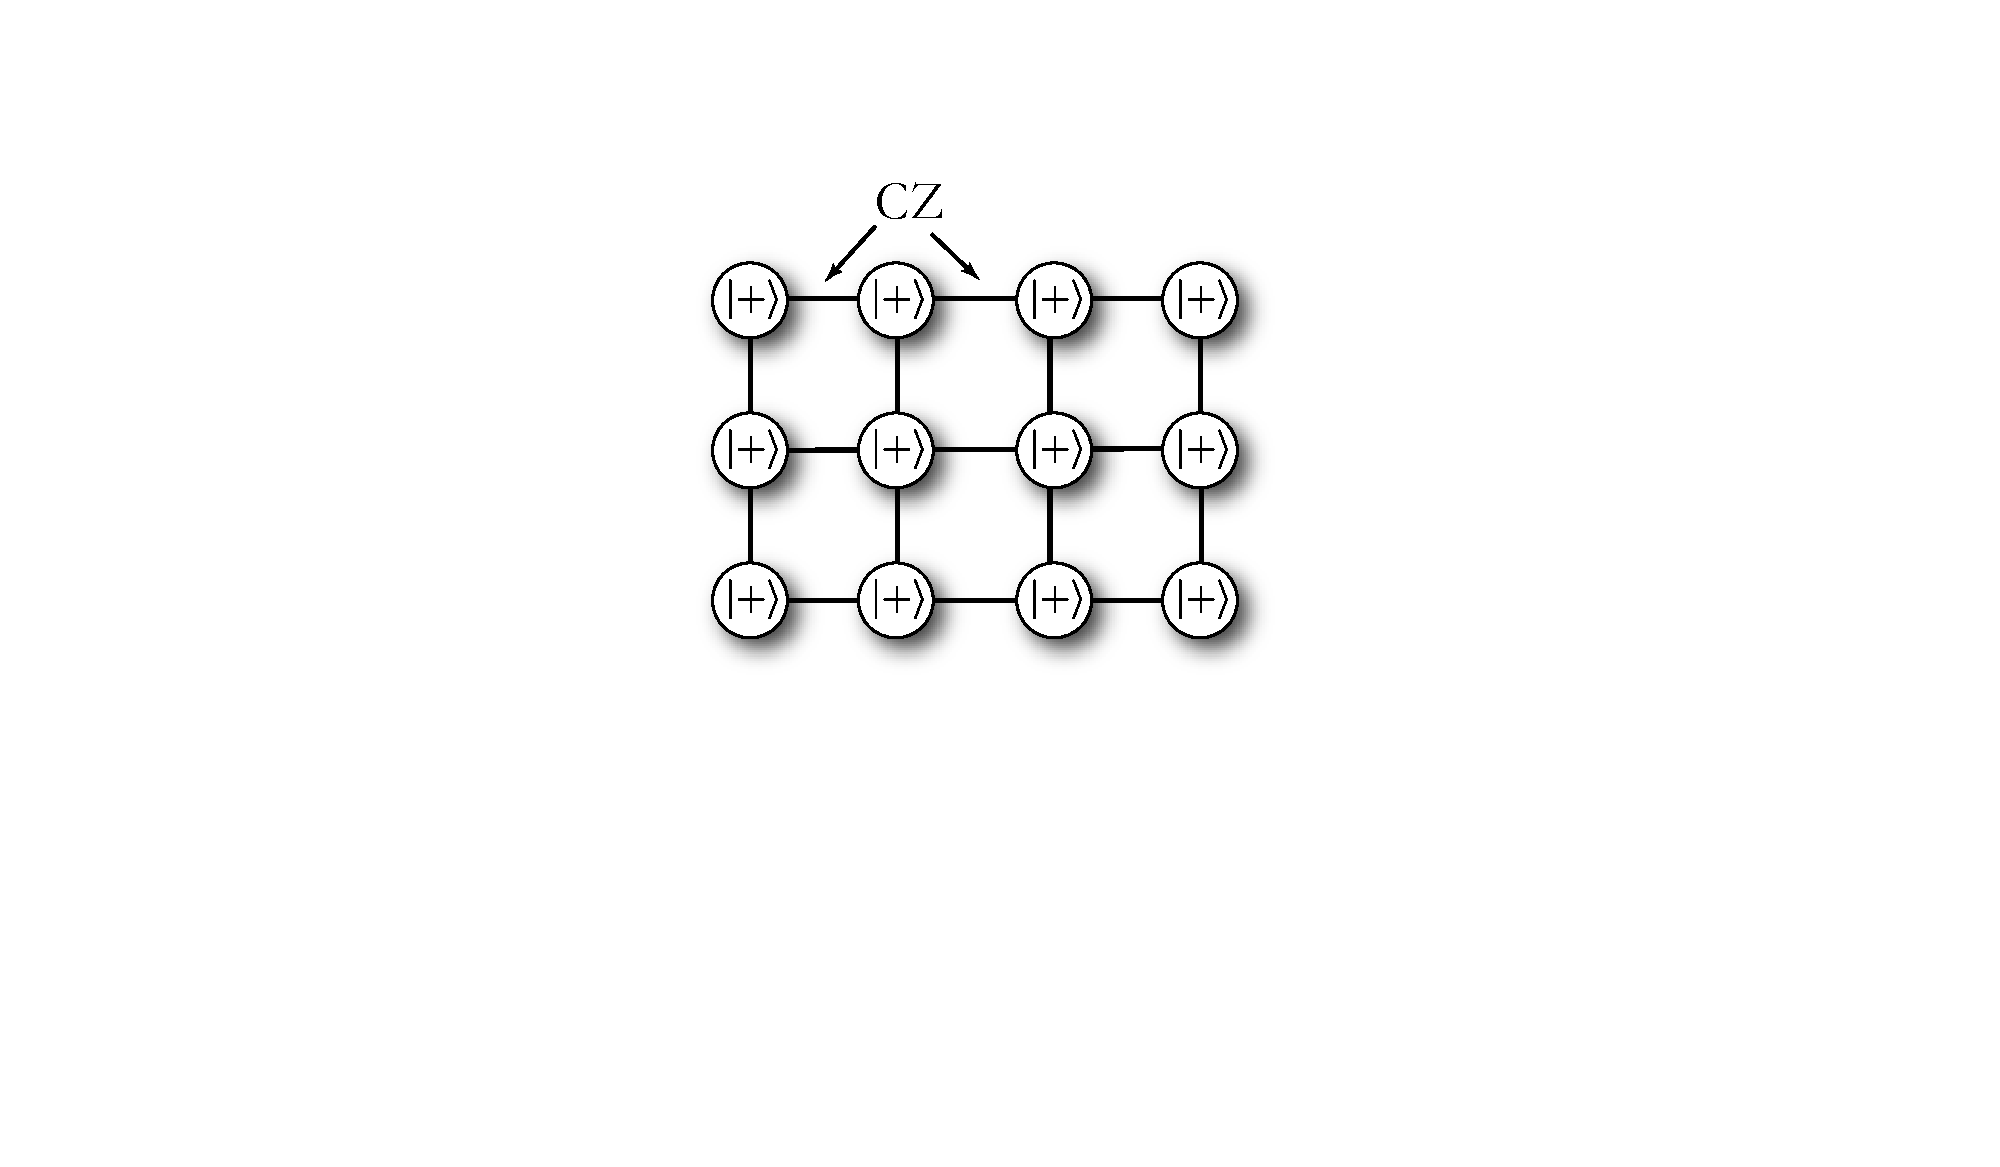
\includegraphics[clip=true, width=0.3\textwidth]{cluster_state}
	\captionspacefig \caption{Example of a \mbox{$4\times 3$} rectangular lattice cluster state. Each vertex in the graph represents a qubit initialised into \mbox{$\ket{+}=\frac{1}{\sqrt{2}}(\ket{0}+\ket{1})$}. Edges represent the application of CZ gates between qubits (CZ gates commute, so the order is unimportant). Of sufficient dimension, states of this topology enable universal measurement-based quantum computation, whereby computation proceeds purely via single-qubit measurements, and all entangling operations have been commuted to the state preparation stage. Because CZ gates commute, the preparation of cluster states is time-independent, and easily implemented in a distributed or parallelised manner. The time-ordering of the single-qubit measurements is dependent on the structure of the graph and the algorithm.} \label{fig:cluster_state}
\end{figure}

Having prepared this state, the computation is implemented purely via a well-orchestrated routine of single-qubit measurements. The order and basis in which they are performed (which depends on previous measurement outcomes in general -- i.e we require fast-feedforward) then stipulates the computation. In the context of distributed computation (Sec.~\ref{sec:dist_QC}), this requires classical communication between nodes.

Mapping a circuit model computation to a cluster state topology can be most na{\" i}vely performed by taking a circuit acting on $n_\mathrm{qubits}$ qubits with depth $n_\mathrm{depth}$, preparing an \mbox{$n_\mathrm{qubits}\times n_\mathrm{depth}$} rectangular lattice cluster, and `etching' the circuit directly into the cluster state substrate. To perform this mapping we choose a universal gate set comprising CZ and single-qubit gates, retaining vertical edges where CZ gates ought to be present, eliminating the remaining vertical edges. Now we have a substrate that looks topologically very much like its equivalent circuit construction, and the computation proceeds chronologically in the same manner. The only conceptual distinction is that in the circuit model gates are directly applied chronologically to the set of qubits, whereas in the cluster state gate teleportation (Sec.~\ref{sec:teleport_gate}) is effectively implemented upon each measurement, with the action of gates accumulating as these teleportations are successively applied. A simple example of this notion is shown in Fig.~\ref{fig:cluster_state_circuit}.

\begin{figure}[!htbp]
	\includegraphics[clip=true, width=0.375\textwidth]{cluster_state_circuit}
	\captionspacefig \caption{Simple example of a cluster state that performs a computation comprising single-qubit operations and a CZ gate between two logical qubits. Let the two horizontal chains represent our two logical qubits. After inputting our input state from the left, we progressively measure out the cluster state qubits chronologically from left-to-right. Upon each single-qubit measurement, the choice of measurement basis teleports the action of a single-qubit gate. These accumulate sequentially. When we reach the point of measuring the two cluster state qubits joined with the vertical edge, the logical qubits accumulate the action of a CZ gate between them, since this is identically what that vertical edge physically corresponds to. Reaching the final two qubits, one from the upper rail and one from the lower, we obtain our two output logical qubits.} \label{fig:cluster_state_circuit}
\end{figure}

The distinctive feature of this model is that all the entangling CZ gates are performed at the very beginning of the protocol, during the state preparation stage. The algorithm itself is purely measurement-based, requiring only single-qubit measurements (no entangling measurements).

An alternate interpretation of the cluster state model is that it is a complicated network of state and gate teleportation protocols (Sec.~\ref{sec:teleport}). Specifically, a CZ gate with a $\ket{+}$ state as a resource, followed by measurement of one of the two qubits acts as a single-qubit teleporter, as shown in Fig.~\ref{fig:single_qubit_teleporter}\footnote{This is an alternative, but equivalent implementation for quantum state teleportation to that presented in Sec.~\ref{sec:teleport}.}. Thus, with a substrate state of CZ gates applied between $\ket{+}$ states, the single-qubit measurements progressively teleport the input state through the graph topology, at each stage accumulating the action of more gates, which are related to the choices of the previous single-qubit measurement bases, and the graph topology.

\begin{figure}[!htbp]
	\begin{align}
		\Qcircuit @C=.7em @R=.4em @! {
		\lstick{\ket{\psi}} & \ctrl{1} & \gate{H} & \meter & & \\
		\lstick{\ket{+}} & \ctrl{0} & \qw & \gate{X} \cwx & \gate{H} & \rstick{\ket\psi} \qw \\
		} \nonumber
	\end{align}
	\captionspacefig \caption{The single-qubit teleporter, based upon a CZ gate, a single-qubit measurement, and classical feedforward.} \label{fig:single_qubit_teleporter} \index{Single-qubit teleporter}
\end{figure}

The cluster state formalism has proven very useful, enabling the development of models for linear optics quantum computing (Sec.~\ref{sec:KLM_univ}), orders of magnitude more efficient than the originally proposed protocol. It has been found that bonding strategies -- i.e the order in which smaller clusters are fused into larger ones when using non-deterministic gates -- plays a major role in resource overhead, and much work has been performed on efficient preparation strategies for various topologies \cite{bib:Nielsen04, bib:BarrettKok05, bib:BrowneRudolph05, bib:BenjaminEisert05, bib:Gross06, bib:RohdeBarrett07, bib:Kieling06, bib:KielingRudolphEisert06, bib:RohdeBarrett07, bib:Kieling07, bib:Campbell07, bib:Campbell07b}.

These cluster states are highly valuable, given their computational power, and the ability to communicate them from Alice, who is able to prepare them, to Bob, who lacks the technology, would be a boon for Bob.

It would be most practical, economical, and resource efficient to have a single, well-equipped server with the ability to prepare such states, who does so on behalf of everyone else, and communicates the fresh cluster states to them over the quantum internet (for a price, perhaps).

Importantly, the preparation of cluster states is readily parallelised. All the entangling CZ operations commute, the order in which they are applied is irrelevant, and a rectangular lattice cluster is completely uniform. Thus, the graphs representing smaller cluster states may be easily `fused' together to form larger cluster states using, for example, CZ gates. Several other types of entangling gates can also be employed, such as polarising beamsplitters -- so-called \textit{fusion gates} \cite{bib:BrowneRudolph05}. This allows the preparation of cluster states to be performed in a `patchwork quilt'-like manner -- a number of nodes each prepare small lattice clusters, they are all put side-by-side, and stitched together using CZ gates. This type of distributed state preparation is a perfect application for in-parallel distributed quantum processing (Sec.~\ref{sec:dist_QC}).

Consider the scenario whereby Alice requests a large cluster state from Bob, but, while she was unable to prepare the cluster state herself, she has the technological ability to perform the measurement-based computation on the state (i.e simple single-qubit measurements). This would effectively bypass the need for secure quantum computation (Sec.~\ref{sec:homo_blind}) on Bob's hardware altogether, enabling computation with \textit{perfect} secrecy, since no foreign parties would be involved in the computation stage, and no secret data is communicated -- only the \textit{substrate} for the computation is communicated, which could be used for any purpose whatsoever. By commuting all the technologically challenging aspects of a quantum computation to the state preparation stage, we can effectively mitigate the need for blind quantum computing entirely, since the `hard work' has been done in advance by the host, and Alice gets to fulfil the computation on her own, completely bypassing poor old Bob, who was just dying to read Alice's secret love letters before processing them into Hallmark cards.

There are several cluster state identities we will utilise later, summarised in Fig.~\ref{fig:cluster_ident}.

\begin{figure}[!htbp]
	\includegraphics[clip=true, width=0.475\textwidth]{cluster_identities} \index{Cluster states!Identities}
	\captionspacefig \caption{Several cluster state identities, demonstrated in the case of linear clusters. (a) a CZ gate between two qubits creates an edge between them in the graph. (b) Measurement of a qubit in the Pauli $\hat{Y}$ basis removes that qubit from the graph, whilst creating new edges between the neighbouring qubits. (c) Measurement of a qubit in the Pauli $\hat{Z}$ basis removes that qubit and any neighbouring edges. (d) Measurement of a qubit in the Pauli $\hat{X}$ basis removes that qubit, leaving one of its neighbours as a `dangling node'.} \label{fig:cluster_ident} 
\end{figure}

When using non-deterministic gates (i.e ones that probabilistically fail) to prepare cluster states\index{Non-deterministic cluster state preparation}, there are approaches to nonetheless preparing ideal cluster states. There have been two main approaches that have become particularly well known. 

The first is to use the ideas of \textit{micro-clusters}\index{Micro-cluster states} and cluster state recycling\index{Cluster states!Recycling} to incrementally build up larger clusters, progressing as a random walk\index{Random walks}, which is biased in the direction of state growth. This approach is discussed in more detail in Secs.~\ref{sec:CS_LO} \& \ref{sec:module}.

The second approach is to borrow techniques from percolation theory\index{Percolation theory} to simply tolerate defects in a cluster state lattice by working around them \cite{Brown}. Specifically, if the defect probability (i.e probability of a missing vertex or edge) is below some \textit{percolation threshold}\index{Percolation threshold}, \mbox{$p_\mathrm{defect}\leq \epsilon_\mathrm{threshold}$}, in the asymptotic limit we are guaranteed that routes exist through the lattice, enabling the required flow of information. This allows defective graphs to be employed for quantum computation.

%
% Adiabatic Quantum Computation & Quantum Annealing
%

\subsection{Adiabatic quantum computation \& quantum annealing} \label{sec:adiabatic_QC} \index{Adiabatic quantum computation} \index{Quantum annealing}

\comment{To do}

%
% Restricted Models for Quantum Computation
%

\subsection{Restricted models for quantum computation} \label{sec:restricted_models} \index{Restricted models for quantum computation}

In the near future we are unlikely to have devices with the full power and versatility of universal quantum computers. Instead, we will gradually evolve towards that challenging goal via many incremental, intermediate steps. Those steps will take us along a path of restricted quantum computers, that solve specific problems of relatively small size, and are not fault-tolerant. Probably we can expect them to contain on the order of hundreds of qubits in the coming few years, as of the time of writing this.

We dedicate Sec.~\ref{sec:NISQ} to discussing these so-called \textit{Noisy Intermediate-Scale Quantum} (NISQ) devices \cite{bib:preskill2018quantum}, speculating on what that might exactly entail for our quantum journey in the near future.

One thing is for certain -- full-fledged quantum computing will remain an extremely ambitious goal for some time, but we will learn a lot from traversing the path towards it, and hopefully uncover new restricted quantum applications along the way.

%
% Fault-Tolerance
%

\subsection{Fault-tolerance}\index{Fault-tolerance}\label{sec:fault_tolerance}

\comment{To do. Help from Simon Devitt.}

In Sec.~\ref{sec:QOS_chap} we discussed QoS\index{Quality of service (QoS)} in the context of quantum networks, where we wish to protect the quantum information being communicated via packets of quantum data. In particular, QEC\index{Quantum error correction (QEC)} allows us to detect and correct errors introduced into quantum data during transmission across noisy channels.

Much more broadly, in the context of an entire quantum computation we will want to achieve the same goal, except that our techniques will need to extend far beyond defending individual quantum states against errors during transmission, but defending an entire computation and all the information residing within it at every stage throughout its execution.

This is achieved by extending techniques from QEC to achieve \textit{fault-tolerant quantum computing}. The primary difficulty here is that a quantum computation is not a passive operation, but involves the successive application of a potentially enormous number of quantum gates, each of which subject to its own error processes, all of which must be mitigated for the computation to succeed.

Because a quantum computation is not a passive operation but highly active, fault-tolerance protocols are also active and it does not suffice to simply perform an encoding at the beginning and error correction at the end. Instead, error correction procedures must be applied repeatedly throughout execution, at each stage projecting the encoded computation onto an error-free state.

As with conventional QEC, this introduces (potentially large, but efficient) overheads associated with encoding logical qubits into fault-tolerant codes. Similarly, there is the notion of \textit{fault-tolerance thresholds}\index{Fault-tolerance!Thresholds} -- thresholds on gate error rates that must be achieved if fault-tolerant execution is to be successful. These thresholds are typically depressingly low (well below 1\%) and are the primary reason humanity has not yet achieved scalable quantum computing.

\latinquote{Aqua vitae.}

%
% Quantum Algorithms
%

\section{Quantum algorithms} \index{Quantum algorithms}\label{sec:quantum_algs}

The ultimate goal of quantum computing is to implement algorithms with a quantum speedup compared to classical algorithms. The degree of speedup achieved varies between algorithms, and it is important to note that not every classical algorithm exhibits any speedup when implemented quantum mechanically.

To provide context for the excitement of quantum computing and motivate interest in their development, we now summarise some of the key quantum algorithms that have been described exhibiting quantum speedup.

%
% Deutsch-Jozsa
%

\subsection{Deutsch-Jozsa} \index{Deutsch-Jozsa algorithm}

The first quantum algorithm demonstrating a provable improvement over the best classical algorithm was the Deutsch-Jozsa algorithm\cite{bib:DeutschJozsa92}. Unfortunately the algorithm solves a very contrived problem, designed for the purposes of demonstrating post-classicality rather than solving a problem of actual practical interest. Nonetheless, the algorithm is straightforward to explain and understand, making it a useful starting point in understanding quantum algorithms and the computational enhancement they may offer.

The algorithm relies on a `black box', referred to as an \textit{oracle}\index{Oracle}, which takes an input bit-string and outputs a single bit, evaluating the function $f(x)$ for the $n$-bit input bit-string $x$. In this contrived problem $f(x)$ is guaranteed to be either \textit{uniform}\index{Uniform function} or \textit{balanced}\index{Balanced function}. In the former case, the output to the oracle is always \mbox{$f(x)=0$} or always \mbox{$f(x)=1$}, but it doesn't matter which, they simply must always be the same. In the latter case, the output is \mbox{$f(x)=0$} for exactly half the inputs $x$, and \mbox{$f(x)=1$} for the other half of $x$, but the ordering of which inputs generate which outputs may be arbitrary. The goal of the algorithm is to determine whether $f(x)$ is uniform of balanced using the least number of queries to the oracle.

While it's clear that the dimensionality of the input state space is exponentially large, $2^n$, it is fairly obvious that a trivial \textbf{BPP} algorithm exists for solving this problem with confidence exponentially asymptoting to unity against the number of oracle queries. We simply evaluate the oracle for randomly chosen inputs. If we measure any occurrences of measurement outcomes that are not all 0 or all 1 we know with certainty that the function must have been balanced. If on the other hand we measure all 0s or all 1s for more than half the input state space $x$, we know with certainty the function was uniform.

However, if the function were balanced, there is the possibility that it might conspire against us to fool us into thinking the function was uniform until we evaluate half plus one of the input states, requiring $O(2^n)$ oracle queries, although this will occur with exponentially low probability against the number of queries. Thus, the algorithm can be approximated with exponential asymptotic certainty in \textbf{BPP}\index{\textbf{BPP}}. But considering the \textit{worst} case\index{Worst case complexity} rather than the \textit{average} case\index{Average case complexity}, we may have to perform an exponential number of evaluations, $O(2^n)$, to know the answer with absolute certainty.

The Deutsch-Jozsa algorithm solves this rather specialised problem in the worst case using only a single quantum evaluation of the oracle.

The algorithm implementing the Deutsch-Jozsa protocol and its circuit diagram are shown in Alg.~\ref{alg:deutsch_jozsa}. The engine room of the algorithm is in the Hadamard transform\index{Hadamard transform}, $\hat{H}^{\otimes n}$, which prepares an equal superposition of all $2^n$ possible input bit-strings $x$, which are then evaluated in superposition by the oracle. To ensure unitarity, the oracle is defined to implement the transformation\footnote{Note that the seemingly more obvious choice of \mbox{$\hat{U}_f\ket{x}=\ket{f(x)}$} is not unitary. This trick of introducing an additional ancillary state to enable unitary construction of arbitrary functions is a common one in quantum algorithm design.},
\begin{align}
	    \hat{U}_f \ket{x}\ket{y} &= \ket{x}\ket{y\oplus f(x)}.
\end{align}
That is, it flips bit $y$ if \mbox{$f(x)=1$} (equivalently addition modulo 2 or an XOR operation). An inverse Hadamard transform subsequently yields a measurement outcome with one of two possibilities:
\begin{itemize}
	\item The 0 and 1 terms outputted from the oracle interfere perfectly constructively, if the function was uniform.
	\item They interfere perfectly destructively, if the function was balanced.
\end{itemize}
Then, with a single-shot measurement of the inverse Hadamard transformed output from the oracle we establish whether $f(x)$ was balanced or uniform with certainty. This exhibits an exponential worst case speedup compared to a randomised classical sampling algorithm (which is classically optimal).

\begin{table}[!htb]
\fbox{\parbox{0.965\columnwidth}{\texttt{ 
function DeutschJozsa(f,n):
\begin{enumerate}
    \item Prepare the \mbox{$n+1$}-bit state,
    \begin{align}
    \ket\psi_0 = \ket{0}^{\otimes n}\ket{1}.	
    \end{align}
    \item Apply the \mbox{$n+1$}-bit Hadamard transform across all qubits,
    \begin{align}
    \ket\psi_1 &= \hat{H}^{\otimes(n+1)}\ket\psi_0 \nonumber \\
    &= \frac{1}{\sqrt{2^{n+1}}} \sum_{x=0}^{2^n-1}\ket{x}(\ket{0}-\ket{1}),	
    \end{align}
    where $x$ denote $n$-bit binary bit-strings, of which there are $2^n$.
    \item Apply the unitary oracle, implementing the transformation,
    \begin{align}
    \hat{U}_f \ket{x}\ket{y} &= \ket{x}\ket{y\oplus f(x)},
    \end{align}
    where $\oplus$ denotes addition modulo 2, yielding,
    \begin{align}
    \ket\psi_2 = \hat{U}_f \ket\psi_1.	
    \end{align}
    \item Apply another Hadamard transform,
    \begin{align}
    \ket\psi_3 = \hat{H}^{\otimes n} \ket\psi_2.
    \end{align}
    \item The full evolution is thus given by,
    \begin{align}
    	\ket\psi_\text{out} = (\hat{H}^{\otimes n}\otimes\hat{I}) \cdot \hat{U}_f \cdot \hat{H}^{\otimes (n+1)}\ket{0}^{\otimes n}\ket{1}.
    \end{align}
	\item Measure the first $n$ qubits to determine the probability of measurement outcome $\ket{0}^{\otimes n}$.
	\item This probability is given by,
	\begin{align}
	P_0 = \left| \frac{1}{2^n} \sum_{x=0}^{2^n-1} (-1)^{f(x)} \right|^2.	
	\end{align}
	\item Depending on whether $f(x)$ was uniform or balanced, the alternating sign terms in this sum interfere constructively or destructively, yielding \mbox{$P_0=1$} or \mbox{$P_0=0$} respectively.
	\item Thus, a single measurement outcome suffices to determine whether $f(x)$ was balanced or uniform.
	\item $\Box$
\end{enumerate}
\begin{align}
\Qcircuit @C=1em @R=1.6em {
    \lstick{\ket{0}^{\otimes n}} & \gate{\hat{H}^{\otimes n}} & \multigate{1}{\hat{U}_f} & \gate{\hat{H}^{\otimes n}} & \meter \\
    \lstick{\ket{1}} & \gate{\hat{H}} & \ghost{\hat{U}_f} & \qw & \\
} \nonumber
\end{align}
}}}
\caption{Deutsch-Jozsa algorithm for evaluating whether the function $f(x)$ implemented by the oracle is balanced or uniform, exhibiting exponential worst case speedup compared to the best classical \textbf{BPP} algorithm.} \label{alg:deutsch_jozsa}
\end{table}

%
% Quantum Search
%

\subsection{Quantum search} \index{Grover's algorithm}

The problem of finding specific entries in unstructured data spaces is a ubiquitous one. This class of \textit{search algorithms} have amongst the broadest applicability of any class of algorithms. Computer scientists have invested excruciating man-hours\index{SJW}\footnote{Presently, most computer science research institutions are equal opportunity employers.} into organising and structuring data so as to minimise the resource overhead (in time and/or space) associated with extracting desired components. However, the methodology for achieving this, and the favourability of associated resource overheads, is highly dependent on the structure of the underlying data, or whether there even is any. To this end, numerous data structures and algorithms have been developed, accommodating for every mutation and variation of the posed problem imaginable. Often, there is a tradeoff between the overheads induced in time and memory, as well as in pre-processing and data structure maintenance requirements.

For example, \textit{hash tables}\index{Hash tables} enable theoretical $O(1)$ lookup times on data with a \textit{key-value pair}\index{Key-value pair} data structure. In a key-value pair each data entry (value) is tagged with a unique identifier (key) used for lookup. The value can observe any structure whatsoever, whereas the key is designed so as to minimise search times. When storing telephone numbers one might represent entries as key-value pairs, where the keys are people's names, and the values their respective telephone numbers. An efficient algorithm for mapping keys to physical memory addresses would imply efficient lookup of telephone numbers by name.

In the absence of a key-value representation one might simply store data in sorted form. However, this requires pre-sorting the entire data space, which may become costly for large data sets, and requires continual rearrangement whenever the data space is modified, making it computationally costly for mutable datasets.

For the end user, who wishes to find data elements, the worst-case data space is one with no order or underlying structure. Suppose we want to find whether a number exists in the telephone directory, but we don't know it's associated name. In this instance, it can easily be seen that the best one can hope for, in terms of algorithmic runtime, is to simply look through the data space brute-force\index{Brute-force} until we find what we are looking for. It is clear that with an unstructured space of $N$ elements, this brute-force search algorithm requires on average $O(N)$ queries to find the desired entry. We call this the \textit{unstructured search problem}.

The brute-force classical algorithm, despite already being technically `efficient' (i.e $O(N)$ linear runtime), could nonetheless become unwieldy for very large datasets. Google doesn't want to exhaustively scan their entire collection of data-centres each time they want to lookup a database element. The quantum search algorithm, first presented by Grover \cite{grover1997quantum}, provides a solution to this problem using only $O(\sqrt{N})$ runtime (oracle queries), a quadratic enhancement. Whilst this falls far short of the exponential quantum enhancement one might have hoped for, which has also shown to be optimal \cite{bennett1997strengths, zalka1999grover}, it is nonetheless still extremely helpful for many purposes, given the broad applications for this algorithm.

We will formulate the quantum search algorithm as an oracular algorithm\index{Oracle}, where the oracle takes as input an $n$-bit string, and outputs 1 if the input matches the entry we are looking for, otherwise 0. This formulation of the problem makes the algorithm naturally suited to solving satisfiability problems (many of which are \textbf{NP}-complete and of great practical interest).

The Grover quantum search algorithm is shown explicitly in Alg.~\ref{alg:quant_search}.

\begin{table}[!htb]
\fbox{\parbox{0.965\columnwidth}{\texttt{ 
function Grover(f,n):
\begin{enumerate}
	\item Using a Hadamard transform, prepare the $n$-qubit equal superposition of all $2^n$ logical basis states,
    \begin{align}
    \ket\varphi &= \hat{H}^{\otimes n}\ket{0}^{\otimes n}	 \nonumber \\
    &= \frac{1}{\sqrt{2^n}}\sum_{x = 0}^{2^n - 1}\ket{x},
    \end{align}
    where $x$ denotes a bit-string of length $n$.
	\item The oracle is defined as a unitary black-box, which tags a target element $T$ using a phase-flip,
	\begin{align}
		\hat{U}_T \ket{x} &= (-1)^{f(x)}\ket{x} \nonumber \\
		&= (\hat{I} - 2\ket{T}\bra{T})\ket{x},
	\end{align}
	where $f(x)=\{0,1\}$ is the black-box function determining whether input $x$ is the target element $T$ (\mbox{$f(x)=1$}) or not (\mbox{$f(x)=0$}).
	\item The Grover diffusion operator\index{Grover diffusion operator} is defined to implement,
	\begin{align}
	\hat{U}_s = \hat{I} - 2\ket{T}\bra{T}.
	\end{align}
    \item repeat $O(N)$ times:
    \setlength{\itemindent}{.2in}
    \item $\ket{\varphi_{i+1}} = \hat{U}_s\cdot\hat{U}_T\ket{\varphi_i}$.
    \setlength{\itemindent}{0in}
    \item $\Box$
    \item \comment{What about measurement stage}
\end{enumerate}
}}}
\caption{.} \label{alg:quant_search}
\end{table}

%
% Optimisation, Satisfiability & NP-Complete Problems
%

\subsection{Optimisation, satisfiability \& \textbf{NP}-complete problems}\index{Optimisation problems}\index{\textbf{NP}-complete problems}\index{Satisfiability problems}

Many readers will have heard of the \textit{travelling salesman problem}\index{Travelling salesman problem}, the task of finding the shortest route through a weighted graph that traverses every vertex. This task is known to be \textbf{NP}-complete.

Many other algorithms are also known to be \textbf{NP}-complete, a number of which that are relevant to networking are discussed in detail in Sec.~\ref{sec:graph_theory}, summarised in Table.~\ref{tab:net_alg_sum}.

Such \textbf{NP}-complete algorithms can be quadratically enhanced in runtime using Grover's algorithm. To see this, note that all \textbf{NP}-complete problems can be efficiently mapped to one another with polynomial resource overhead (see Fig.~\ref{fig:complexity_classes}). Thus, we can restrict ourselves to considering the satisfiability problems\index{Satisfiability problems} discussed above -- the archetypal \textbf{NP}-complete problems. An example of the {\sc 3-SAT} problem\index{3-\textsc{SAT} problem }, which is \textbf{NP}-complete, is shown in Fig.~\ref{fig:3SAT}.

\begin{figure}[!htb]
\includegraphics[width=0.3\textwidth]{3SAT}
\caption{Digital circuit for an instance of the {\sc 3-SAT} problem. Each or the OR gates is input with some combination of the input bits or their compliments (i.e with a NOT gate). Each of these is referred to as a `clause', of which there are 4 in this example, but could be any number in general. The final AND gate requires that all clauses be simultaneously satisfied in order to yield a final output of `1'. The goal of the problem is to find an input bit-string that yields an output of `1'. In general, this may require exhaustively searching over the entire space of input states via brute-force, which exhibits time-complexity exponential in the length of the bit-string. This problem is proven to be \textbf{NP}-complete.} \label{fig:3SAT}	
\end{figure}

Now, by defining an oracle that implements a polynomial-time algorithm on $n$ qubits, a Grover search over the input space of $2^n$ configurations will determine the satisfying input to the oracle for a given desired output, which acts as the tagged element within the search algorithm. The Grover search yields a quadratic speedup for this search compared to a brute-force classical search, therefore requiring only $O(2^{n/2})$ oracle calls. While this is short of the exponential speedup one might hope for, a quadratic speedup can nonetheless be very significant for large instances of the problems.

Some problems in even harder classes than \textbf{NP}-complete can in some instances be \textit{approximated} using the same approach. The key to solving such problems is to define an oracle that attributes a \textit{score} to a given input, rather than a yes/no answer to satisfiability, and answers `yes' or `no' depending on whether that score is above some defined threshold. As an illustrative example, consider the optimisation of, say, a complex traffic network, where the goal is to maximise flow through the network. Then we might define our score to be some flow metric for the network's graph.

We then apply a Grover search repeatedly, each time incrementing this threshold until the algorithm outputs `no'. Then we know that the last input had the highest score. The reason this approach is \textit{approximate} rather than \textit{exact} is that defining such a score-oracle mightn't be always efficiently implemented, or maybe it mightn't make sense at all to define score measures for a given problem.

%
% Quantum Simulation
%

\subsection{Quantum simulation} \index{Quantum chemistry}\index{Quantum simulation}\index{Hamiltonian simulation}\label{sec:quantum_sim_alg}

\comment{To do - Zuen}

\comment{Discuss quantum chemistry as leading application}

%
% Integer Factorisation
%

\subsection{Integer factorisation} \index{Shor's algorithm}\index{Hidden subgroup problem}\index{Period-finding algorithm}\index{Discrete logarithm algorithm}

\comment{To do - Heliang}

\comment{Mention relationship to hidden subgroup, period-finding, and discrete-log problems}

While this algorithm is known to reside in \textbf{BQP}, it is strongly believed not to be \textbf{BQP}-complete. Similarly, while it is known to reside in \textbf{NP}, it is strongly believed not to be \textbf{NP}-complete, thereby placing it in the `limbo zone' of \textbf{NP}-intermediate complexity.\index{\textbf{NP}-intermediate}

%
% Quantum Machine Learning
%

\subsection{Quantum machine learning} \index{Quantum machine learning}

\comment{To do - Chris}

%
% Topological Data Analysis
%

\subsection{Topological data analysis} \index{Topological data analysis}

\cite{SethTDA}

\begin{figure}[!htb]
\includegraphics[width=0.47\textwidth]{TDA}
\caption{(top) Simplices are constructed as fully connected subgraphs of the data of different dimensions. (bottom) A distance cutoff is applied to create edges within a scatterplot of raw data, from which the simplicial complex is constructed.} \label{fig:TDA_simplex}	
\end{figure}

\comment{To do}

%
% Linear Systems
%

\subsection{Linear systems} \index{Linear systems}

\comment{To do}

\comment{Example: recommendation algorithm where sampling the vector yields, with high probability, a recommendation that is a good one, without having to explicitly know the entire solution vector.}

%
% Intermediate Models for Quantum Computation
%

\subsection{Intermediate models for quantum computation}

\comment{To do}

\index{Galton board}
\index{Sampling problems}

Sec.~\ref{sec:BS}
\comment{Boson-sampling and IQP. Other sampling problems.}

\begin{figure}[!htb]
\includegraphics[width=0.3\textwidth]{galton_board}
\caption{The Galton board yields a very simple classical sampling problem. Balls (red) are input at the top and allowed to fall freely through the pyramid network of pegs (grey), at which balls bounce to the left or right with 50\% probability. At the output the balls are collected into buckets, which populate according to a binomial distribution\index{Binomial distribution}. The computational problem is to produce statistically accurate samples from such a device, which classically is efficiently implemented by sampling the binomial distribution.}	\label{fig:galton_board}\index{Galton board}
\end{figure}


\latinquote{Sic semper tyrannis.}

%
% Physical Architectures For Quantum Computing
%

\section{Physical architectures for quantum computing} \label{sec:archs_QC} \index{Physical architectures}

\dropcap{T}{he} models for quantum computation introduced in the previous section are abstractions of algorithms in terms of elementary operations. But elementary operations must ultimately be physically realised. There are countless physical architectures for realising quantum computations, far too many to describe here, each with their own advantages and disadvantages, and it is far from clear which physical architecture(s) will ultimately win the quantum race.

Here we will summarise some of the physical architectures most applicable to networking. Since we reasonably anticipate that future quantum networking will be optically mediated, we focus on pure-optical and hybrid-optical architectures, on the basis that these will naturally lend themselves to optical interfacing.

%
% Universal Linear Optics
%

\subsection{Universal linear optics} \label{sec:KLM_univ} \index{Universal linear optics quantum computation}\index{Knill-Laflamme-Milburn (KLM)}

With single-photon encoding of qubits in the quantum network, the obvious architecture to implement quantum computation is linear optics quantum computing (LOQC) \cite{bib:KLM01} (KLM), since the states being processed by the computer are of the same form as the states traversing the network. See \cite{bib:Kok05, bib:KokLovettBook} for excellent introductions to this what has become a very broad and exciting field.

LOQC allows universal quantum computing to be implemented using single-photon polarisation or dual-rail encoding, with only linear optics interactions, i.e beamsplitter/phase-shifter networks \cite{bib:Reck94}, with the addition of quantum memory, and fast-feedforward, whereby some photons are measured, and the remaining part of the optical circuit is dynamically reconfigured based on the measurement outcomes. The former is readily available technology today, and elementary demonstrations have been performed \cite{bib:OBrien03, bib:carolan2015universal}, but the latter two have proven to be somewhat more challenging.

Originally it was believed that universal optical quantum computation, specifically the implementation of 2-qubit entangling gates (such as CNOT or CZ gates), would require extremely (and unrealistically) strong optical non-linearities that implement a non-linear sign-shift (NS) gate,
\begin{align} \label{eq:NS_trans}\index{Non-linear sign-shift (NS) gate}
NS: \alpha\ket{0}+\beta\ket{1}+\gamma\ket{2}\to\alpha\ket{0}+\beta\ket{1}-\gamma\ket{2},
\end{align}
in the photon-number basis, up to normalisation (which is determined by the post-selection success probability). That is, it applies a $\pi$ phase-shift to only the $\ket{2}$ component of a photon-number superposition. The breakthrough result by KLM demonstrated that this is in fact not the case at all. Instead, the NS gate can be implemented non-deterministically using post-selected linear optics. Two such NS gates allow the construction of a single CZ gate. The construction of the KLM NS and CZ gates are shown in Figs.~\ref{fig:KLM_gate} \& \ref{fig:KLM_explain}. Equivalently, a CNOT gate may be trivially constructed via conjugation by Hadamard gates, based on the identity \mbox{$\hat{H}\hat{Z}\hat{H}=\hat{X}$}.

\begin{figure}[!htbp]
\includegraphics[clip=true, width=0.42\textwidth]{KLM_gate}
\captionspacefig \caption{(a) A KLM CZ gate, employing dual-rail encoding, constructed from two non-linear sign-shift (NS) gates, which apply a $\pi$ phase-shift to only $\ket{2}$ terms in the photon-number basis. (b) Construction of the non-deterministic linear optics NS gate. Two ancillary states -- one $\ket{1}$ and one $\ket{0}$ -- are employed, and two photo-detectors post-select upon detecting $\ket{1}\bra{1}$ and $\ket{0}\bra{0}$ respectively. The beamsplitter reflectivities in (a) are 50:50, and in (b) chosen such that the amplitudes obey Eq.~(\ref{eq:NS_trans}).}. \label{fig:KLM_gate} \index{Knill-Laflamme-Milburn (KLM)}\index{Non-linear sign-shift (NS) gate}
\end{figure}

\if 2\pubmode
	\begin{figure}[!htbp]
	\includegraphics[clip=true, width=0.43\textwidth]{KLM_optical_paths_long}
	\captionspacefig \caption{Evolution of the four logical basis states through the KLM CZ gate. The NS gates do nothing in the first three cases, since they are operating only on vacuum and single-photon terms, which are left unchanged by the NS gate. In the last case, where both control and target are on, HOM interference results in photon bunching after the first beamsplitter, thereby creating two-photon terms. These terms inherit the $\pi$ phase-shift from the NS gate transformation, after which the final beamsplitter reverses the HOM photon bunching, yielding the same logical basis state with an acquired $\pi$ phase-shift.} \label{fig:KLM_explain} \index{Knill-Laflamme-Milburn (KLM)}\index{Controlled-Z (CZ) gates}
	\end{figure}
\else
	\begin{figure*}[!htbp]
	\includegraphics[clip=true, width=0.9\textwidth]{KLM_optical_paths}
	\captionspacefig \caption{Evolution of the four logical basis states through the KLM CZ gate. The NS gates do nothing in the first three cases, since they are operating only on vacuum and single-photon terms, which are left unchanged by the NS gate. In the last case, where both control and target are on, HOM interference results in photon bunching after the first beamsplitter, thereby creating two-photon terms. These terms inherit the $\pi$ phase-shift from the NS gate transformation, after which the final beamsplitter reverses the HOM photon bunching, yielding the same logical basis state with an acquired $\pi$ phase-shift.} \label{fig:KLM_explain} \index{Knill-Laflamme-Milburn (KLM)}\index{Controlled-Z (CZ) gates}
	\end{figure*}
\fi

Clearly this non-determinism is of immediate concern, since concatenating multiple gates would have exponentially decreasing success probability, making the protocol inefficient -- if the probability of a single gate succeeding is $p$, and we require that a circuit comprising $n$ of them all succeed, the success probability is clearly $p^n$.

The first key observation then is that gate teleportation can be used to shift this non-determinism to a resource state preparation stage, as described in detail in Sec.~\ref{sec:teleport_gate}. However, this is not the end of the story, since gate teleportation requires Bell state projections, which are themselves non-deterministic using purely linear optics (either using PBSs or CNOT gates). \latinquote{Ignotum per ignotius}.

The final insight provided by KLM is that by concatenating these non-deterministic CNOT gates, we can inductively build up higher-level CNOT gates with ever increasing success probabilities, asymptoting to unity with high- (but polynomial-) depth concatenation. By combining these key insights, KLM were able to show that near-deterministic CNOT gates can be constructed using an efficient (polynomial) resource overhead, thereby enabling efficient universal quantum computation\footnote{Note that all single-qubit gates are trivially and deterministically implemented using wave-plates or beamsplitters, for polarisation or dual-rail encoding respectively. Thus, we need only concern ourselves with the challenges associated with implementing 2-qubit entangling gates.}. A sketch of the general KLM formalism is shown in Fig.~\ref{fig:KLM_protocol}.

\begin{figure}[!htbp]
\includegraphics[clip=true, width=0.28\textwidth]{KLM}
\captionspacefig \caption{KLM architecture for universal LOQC. $n_L$ optical modes are associated with logical qubits in the state $\ket{\psi_L}$, with the remaining $n_A$ modes acting as ancillary states, $\ket{\psi_A}$. A round of passive linear optics is applied, $\hat{U}_1$. Then the ancillary modes are measured, yielding some set of measurement outcomes $m_1$. These are classically processed to determine what the next round of passive linear optics, $\hat{U}_2$, ought to be. This repeats some polynomial number of times, from which an arbitrary quantum computation can be implemented. The \textsc{BosonSampling} and quantum walk models are equivalent to taking just the first stage of this protocol: one round of input state, passive linear optics, and measurement.} \label{fig:KLM_protocol}\index{Knill-Laflamme-Milburn (KLM)}
\end{figure}

Evolution via linear optics implements transformations of the form of Eq.~(\ref{eq:LO_unitary_map}), and may be implemented using the experimental architectures described in Sec.~\ref{sec:LO_ev_archs} and Fig.~\ref{fig:LO_archs}.

The measurements are implemented simply by number-resolved photo-detectors, implementing measurement projectors of the form \mbox{$\hat\Pi_n=\ket{n}\bra{n}$}, for the measurement outcome of $n$ photons (Sec.~\ref{sec:photo_detection}).

Since the original presentation of a universal LOQC gate set by KLM, numerous alternate implementations have been presented and experimentally demonstrated, with various pros and cons \cite{bib:Ralph01, bib:Pittman01, bib:Ralph02, bib:Knill02, bib:Pittman03, bib:MorYoran06}.

Significant progress is being made on reconfigurable, integrated LOQC devices \cite{bib:carolan2015universal}, but switching times remain orders of magnitude slower than that required for fast-feedforward. The resource overhead associated with overcoming the non-determinism of entangling gates is substantial in the original KLM proposal. But despite being improved upon by cluster state approaches, to be discussed next (Sec.~\ref{sec:CS_LO}), resource scaling remains daunting. It therefore seems most likely that certain elements from LOQC might be combined into hybrid architectures, to be discussed in detail in Sec.~\ref{sec:hybrid}.

%
% Cluster State Linear Optics
%

\subsection{Cluster state linear optics} \label{sec:CS_LO} \index{Cluster states}

Although the original KLM scheme is universal, and `efficient'\footnote{From a purely computer scientist's definition of `efficient = polynomial'\index{Efficiency}.}, resource usage can be reduced by orders of magnitude by combining concepts from LOQC with the cluster state formalism (Sec.~\ref{sec:CSQC}) or related concepts \cite{bib:YoranReznik03, bib:Nielsen04, bib:BrowneRudolph05, bib:GilchristHayes05, bib:Lim05, bib:LimBarrett05}.

Specifically, instead of using our non-deterministic KLM CZ gates within the circuit model formalism, they could be employed for the preparation of cluster states, since after all a CZ gate directly creates an edge in a cluster state graph.

We now review approaches for cluster state-based LOQC using non-deterministic entangling gates. A further discussion of this topic continues in Sec.~\ref{sec:module}, where we introduce modularised quantum computing from a cluster state perspective also using non-deterministic gates. We recommend beginning this topic here, and then skipping ahead to Sec.~\ref{sec:module} for continued discussion if interested.

%
% Fusion Gates
%

\subsubsection{Fusion gates}\label{sec:fusion_gates}\index{Fusion!Gates}

As introduced in Sec.~\ref{sec:CSQC}, a cluster state may be defined by the action of CZ gates upon a graph of qubits initialised into the $\ket{+}$ state. As we saw in the previous section, implementing these CZ gates is troublesome using linear optics, as it is non-deterministic and carries the burden of a large resource overhead. Nonetheless, it was shown early on \cite{NielsenOptCS} that by combining non-deterministic CZ gates with the cluster state formalism yields LOQC protocols far more efficient than the original KLM protocol for LOQC.

It was then noted \cite{BrowneRudolph} that CZ gates aren't required at all for the preparation of optical cluster states. Instead, parity measurements (Sec.~\ref{sec:bell_proj})\index{Bell measurements} operating in a rotated basis may be used to fuse smaller cluster states into larger ones, albeit acting destructively on two of the qubits, and also being non-deterministic, with a success probability of $1/2$. These gates have become known as \textit{fusion gates}, of which there are two types:
\begin{itemize}
	\item Type-I: destroy only a single photon, but require efficient number-resolved detection.
	\item Type-II: destroy two photons, but only require on/off detectors, since the gate succeeds upon coincidence events only and preserves photon-number.
\end{itemize}
Both types of gates have several highly favourable characteristics:
\begin{itemize}
	\item Unlike the KLM CZ gate, only HOM stability is required (Sec.~\ref{sec:opt_stab}). At no stage in the cluster state preparation procedure is any interferometric (i.e wavelength-scale) stability required.
	\item Gate failure is heralded by measurement of the wrong photon-number.
	\item Gate failure measures the respective qubits in the computational basis, thereby simply removing those qubits from the cluster state graph, whilst preserving the remainder of the state, which can be `recycled'\index{Cluster states!Recycling} for reuse.
\end{itemize}

The explicit construction of the linear optics fusion gates is shown in Fig.~\ref{fig:fusion_gates}.

\begin{figure}[!htbp]
\includegraphics[clip=true, width=0.4\textwidth]{fusion_gates}
\captionspacefig \caption{Linear optics cluster state fusion gates for polarisation-encoded photons. Both type-I and type-II gates employ a single polarising beamsplitter to mediate the entangling measurement. The black bars represent Hadamard gates in the polarisation basis (waveplates). The type-I gate only measures a single photon, the other freely exiting the gate, which forms a part of the final cluster state. The type-II gate consumes two photons. Because the type-I gate does not measure in coincidence, as per the type-II gate, it requires number-resolved photo-detection, whereas bucket detectors suffice for type-II.} \label{fig:fusion_gates}
\end{figure}

%
% Fusion Strategies
%

\subsubsection{Fusion strategies} \index{Fusion!Strategies}

If a large cluster state has $n$ edges in its graph, single-shot state preparation will succeed with probability $p^n$ if individual gates succeed with probability $p$, implying that on average $1/p^n$ attempts will need to be made until success. Clearly this exponentiality doesn't lend itself to efficient implementation.

Thankfully, cluster states needn't be prepared in a single shot, since individual gate failures do not destroy the entire graph, but rather only cause localised damage to the graph in the vicinity of the gate.

Despite their non-determinism, numerous authors have examined approaches for efficiently preparing arbitrarily large cluster states using these destructive, non-deterministic gates \cite{nielsen, kieling, rohdebarrett, kokBuffer, ???}. We refer to these schemes as `fusion strategies' -- simple algorithms for how to arrange qubits geometrically and the order in which to attempt bonding them.

These principles can be extended beyond LO to other schemes where entangling gates are inherently non-deterministic or sometimes fail in a heralded manner, e.g hybrid architectures (Sec.~\ref{sec:hybrid}), where a beamsplitter mediates entanglement via which-path erasure, but only successfully projects onto an entangled state with probability 1/2.

The key feature of all these fusion strategies is to employ `micro-clusters'\index{Micro-cluster states} as a primitive resource, which enable multiple bonding attempts between them via redundant vertices. We will now outline several of these schemes.

%
% Linear Clusters
%

\paragraph{Linear clusters}\index{Linear cluster states}

We begin with discussion of linear clusters as these are a particularly useful primitive resource for more advanced strategies. We briefly sketch out the formalism introduced by \cite{bib:RohdeBarrett07} for linear state preparation, which is applicable to a number of different variants of entangling gates.

A key observation was that although numerous strategies yield efficient state preparation, exact efficiencies are highly dependent on the ordering of bonding operations -- which clusters do we choose to bond together first?

Consider a non-deterministic KLM-type CZ gate\footnote{In reality, no one would use KLM-type gates for preparing cluster states, owing to their complexity compared to fusion gates. Rather, we use this gate for illustrative purposes, since its operation upon success and failure are very simple for exposition.}, which upon failure destroys its two input photons by measuring them in the computational $\hat{Z}$-basis, and leaves the number of qubits unchanged upon success and bonds them together.

To analyse the operation of such a non-deterministic protocol, we begin by defining a vector $\vec{n}_t$ at time $t$, which stores purely classical information. Specifically, the vector tells us how many clusters of every length we have stored in memory (except single-qubit clusters, which we assume `come for free'\footnote{As in beer.\index{Beer}}). For example, the second element of the vector tells us how many 3-qubit linear clusters we have in our possession.

We then define a strategy, $\mathcal{S}$\index{Fusion!Strategies}, for choosing clusters we have stored and bonding them together to form larger clusters. The strategy acts on our cluster vector and updates it accordingly,
\begin{align}\index{Update rules}
\vec{n}_{t+1} = \mathcal{S}(\vec{n}_t).
\end{align}
That is, the length vector can be thought of as a series of `buckets' containing clusters of different lengths, and the strategy simply probabilistically shuffles the contents of the buckets around each time it is applied. The process can be thought of as a random walk\index{Random walks}, guided by a probabilistic update rule. Fig.~\ref{fig:linear_cs_strategy} outlines the protocol.

\begin{figure}[!htbp]
	\includegraphics[clip=true, width=0.475\textwidth]{linear_cluster_state_strategies}
	\captionspacefig \caption{Protocol for preparing linear cluster states using non-deterministic entangling gates and quantum memory. Each `bucket' holds a resource of micro-clusters of a given length, represented by the vector $\vec n$. Beginning with a resource of single qubits we repeatedly attempt bonding operations between micro-clusters in the buckets, according to a fusion strategy, $\mathcal{S}$. Proceeding as a biased random walk, the contents of the buckets shuffle around until ultimately (hopefully) clusters of the target length $N$ are prepared and steadily flow out as output at rate $r$ clusters per update operation. We assume a free supply of single qubits as a resource.}\label{fig:linear_cs_strategy}
\end{figure}

The strategy description, $\mathcal{S}$, is also responsible for taking care of updating the elements of $\vec{n}$ according to an update rule, which dictates how many photons are lost or gained upon success or failure of the non-deterministic gate. For example, the CZ gate we have employed here for our toy model destroys two qubits upon failure, but upon success creates a cluster of length given by the sum of the lengths of the clusters acted upon by the gate.

We are then interested in the \textit{rate}\index{Cluster states!Preparation rate}, $r$, at which large clusters are output from the protocol. This is simply extracted by defining a single parameter which counts the number of clusters in $\vec{n}$ above some predetermined target length, and normalises it by the total time taken to reach that point. The rate parameter converges asymptotically for long runtimes. Formally, the rate of preparation is given by,
\begin{align}
r = \lim_{t\to\infty} \frac{N_t}{t},
\end{align}
where $N_t$ is the total number of clusters of length greater than the target length at time $t$. The preparation rate is bounded by \mbox{$0\leq r\leq1$}. If the rate $r$ converges to a positive, finite value in the limit of large $t$, this implies state preparation proceeds in linear time and is therefore efficient.

This completes the theoretical analysis for different strategies and gate types, allowing us to explore different approaches tailored to different physical systems and their varying gate implementations.

One of the key outcomes was that a \textsc{Balanced} strategy\index{Balanced strategy} is optimal in terms of preparation rate. This is simply a strategy which preferentially always bonds clusters of equal length, beginning with the largest ones available. Asymmetric strategies, which bond clusters of differing lengths were found to be far less efficient.

Example simulated state preparation rate results are shown in Fig.~\ref{fig:linear_cluster_state_r} for various types of entangling gates and gate success probabilities.

\begin{figure}[!htbp]
\includegraphics[clip=true, width=0.475\textwidth]{linear_cluster_state_rates}
\captionspacefig \caption{Linear micro-cluster preparation rates for three different types of entangling gates as described in \cite{bib:RohdeBarrett07}, against gate success probability, $p_\mathrm{gate}$. Here a \textsc{Balanced} fusion strategy is employed, whereby we only attempt to join clusters of equal length, always prioritising the largest ones available. This strategy was empirically found to perform better than any asymmetric strategies.}\label{fig:linear_cluster_state_r}
\end{figure}

%
% Lattice Clusters
%

\paragraph{Lattice clusters}\index{Lattice cluster states}

As we learnt from Sec.~\ref{sec:CSQC}, linear cluster states are not universal for quantum computation. What is required is lattices, where the rows and columns respectively map to logical qubits and time in the circuit model. There are numerous approaches one could employ to assemble such lattice clusters using non-deterministic gates, however the easiest to treat for illustrative purposes is to take a resource of linear clusters, prepared as described earlier, and weld them together according to some algorithm, enabling more complex two-dimensional topologies.

The central strategy is similar as for linear clusters -- we construct recyclable micro-clusters, which enable multiple bonding attempts, since gate failures only cause localised damage. The key difference now is that these redundant vertices must emanate in multiple directions so as to allow the more complex 2D topology.

Fig.~\ref{fig:micro_clusters} illustrates several topologies for micro-clusters, beginning with the linear micro-cluster that we employed previously for preparing 1D clusters, and two variations of micro-clusters that can be employed for 2D state preparation.

\if 2\pubmode
\begin{figure}[!htbp]
\includegraphics[clip=true, width=0.2\textwidth]{micro_clusters_long}
\captionspacefig \caption{(a) Linear, (b) plus ($+$), and (c) star micro-cluster states.}\label{fig:micro_clusters}\index{Linear micro-cluster states}\index{Plus micro-cluster states}\index{Star micro-cluster states}\index{Micro-cluster states}
\end{figure}
\else
\begin{figure*}[!htbp]
\includegraphics[clip=true, width=0.7\textwidth]{micro_clusters}
\captionspacefig \caption{(a) Linear, (b) plus ($+$), and (c) star micro-cluster states.}\label{fig:micro_clusters}\index{Linear micro-cluster states}\index{Plus micro-cluster states}\index{Star micro-cluster states}\index{Micro-cluster states}
\end{figure*}
\fi

The $+$-cluster\index{Plus micro-cluster states} simply comprises four linear clusters emanating in the four directions, welded together at a central vertex. It's self-evident how this is subsequently applied to 2D state preparation -- we lay out the $+$-clusters in a grid, and attempt nearest neighbour bonding in each direction for every neighbouring pair of micro-clusters.

The star-cluster\index{Star micro-cluster states} similarly allows multiple bonding attempts in each direction. But now the dangling bonds are not uniquely associated with a particular direction, and may therefore be utilised when bonding to a neighbouring micro-cluster in any direction. This implies a modest efficiency improvement, since leftover vertices in any given direction needn't be wasted upon a successful bond in that direction. However, these micro-clusters are not as efficient to prepare as the $+$-clusters, since they do not straightforwardly arise from two fused linear clusters, which are highly efficient to prepare. Rather they must be prepared via a sequence of repeated successful bonding operations to the central node, where a single gate failure destroys the entire state.

In addition to an efficiency improvement in terms of the number of required physical qubits, minimising the number of redundant qubits that must be removed via $\hat{Y}$ measurements upon completion of the bonding strategy has another key benefit -- error accumulation \cite{RohdeMunroEtal}. Whenever a cluster state qubit is measured, the action of any error process that acted on that qubit will be teleported to its neighbour(s). For example, if we measure the first qubit in a linear cluster, which was previously acted upon by a depolarising channel\index{Depolarising channel}, the depolarisation process will be teleported to the neighbouring second qubit in the cluster. Thus, with high levels of redundancy, although this increases our chances of successfully joining two micro-clusters, it similarly increases the accumulation of errors. There is therefore a direct tradeoff between two undesirable error mechanisms -- gate failure, and logical errors. This tradeoff must be carefully managed in a real-world implementation.

Having made this observation about error accumulation, is there a topology that is optimal? Yes there is -- the so-called snowflake cluster, shown in Fig.~\ref{fig:snowflake_graph}. He we take the $+$-cluster topology and replace the linear clusters emanating in each direction with binary tree graphs of some depth, $d$. This variation of micro-clusters has been studied in great detail both in optical and non-optical contexts \cite{SimonBenjaminPapers}.

The endpoints (leaves) of each tree now provide the bonding opportunities for joining two neighbouring micro-clusters. There are $O(2^d)$ such opportunities. The bonding attempts proceed as expected, always exploiting the trees' outermost leaves.

Now the key feature is that when two sub-trees are successfully bonded via their leaves we do not need to measure out \textit{all} the leftover redundant vertices to reduce the graph to the desired residual topology. Instead we can `prune' away entire sub-trees by performing $\hat{Z}$ measurements at the base of their trunks. All vertices above the trunk will thereby be detached from the graph and needn't all be individually measured. Correspondingly, any error processes that had acted on the pruned vertices will not be teleported onto the main cluster, only the measurements acting on the trunks will contribute.

\begin{figure}[!htbp]
\includegraphics[clip=true, width=0.475\textwidth]{microcluster_snowflake}
\captionspacefig \caption{Snowflake micro-cluster comprising a binary tree structure, with depth \mbox{$d=7$}. Multiple copies of this micro-cluster can be placed side-by-side and fused together via attempting to bond the most outward available leaf qubits from neighbouring clusters. The tree structure allows excess qubits to be `pruned' via their trunks rather than leaves, bypassing the need to measure out every single leftover qubit, as is the case, for example, for $+$-clusters. This reduces the number of required pruning measurements from linear to logarithmic, similarly reducing the accumulation of errors associated with pruned qubits.} \label{fig:snowflake_graph}\index{Snowflake micro-cluster states}
\end{figure}

Formally, for a linear subgraph of length $n$, there will be $O(n)$ leftover redundant qubits on average, which must \textit{all} be measured out using $\hat{Y}$ measurements. Thus, the residual state will have accumulated the action of $O(n)$ independent error processes. On the other hand, for a snowflake subgraph, the trees' depth scales as \mbox{$d=O(\log n)$}, and therefore at most \mbox{$O(\log n)$} qubits must be measured to prune away unwanted branches. Fig.~\ref{fig:snowflake_pruning} presents an example of how the pruning process works.

\begin{figure}[!htbp]
\includegraphics[clip=true, width=0.35\textwidth]{snowflake_pruning}
\captionspacefig \caption{Pruning snowflake micro-clusters\index{Snowflake micro-cluster states} upon successful fusion of their outer leaves. Green indicates where the successful fusion operation took place. To remove all redundant nodes we measure the qubits marked in blue in the $\hat{Y}$-basis and the ones marked in red in the $\hat{Z}$ basis. This will discard all the other qubits marked in grey, modulo the two root qubits at the far top and bottom, which are left with a direct link between them. The total number of measured qubits scales logarithmically with the number of leaves.}\label{fig:snowflake_pruning}	
\end{figure}

Keeping in mind that for an error process with error rate $p$, the net probability of an error occurring for $m$ independent channels is \mbox{$1-p^m$}, thus reducing $m$ from linear to logarithmic is highly favourable in terms of the accumulation of errors.

%
% On-Demand Cluster State Preparation
%

\paragraph{On-demand cluster state preparation}\index{On-demand cluster state preparation}

A beautiful feature of the cluster state model is that the entire cluster needn't be prepared in its entirety for computation to proceed. Instead the state can be grown via the fusion of additional qubits on-demand as the computation proceeds. This arises simply because all the entanglement in the graph is nearest neighbour only, i.e very short-range. So long as a gate failure doesn't lay its fingers on the leftmost column of qubits in the cluster we are in business. This means fewer quantum memories are required, which are very challenging optically. In non-optical, specifically matter qubit systems, this additionally means that physical qubits can be reused on-the-fly.

The computation therefore proceeds as alternating applications of:
\begin{enumerate}
	\item Measure the leftmost column of physical qubits to evolve the computation by a single step.
	\item Bond on a new column of qubits to the rightmost column.
\end{enumerate}
The qubits in between the left and rightmost columns act as a buffer to give us some leeway when bonding operations fail. The architecture is shown in Fig.~\ref{fig:on_demand_cs}.

\begin{figure}[!htbp]
\includegraphics[clip=true, width=0.475\textwidth]{on_demand_cluster_states}
\captionspacefig \caption{On-demand cluster state preparation. Every time a column of computational qubits are measured away from the lefthand side, thereby evolving the computation by a single step, we dynamically bond on a fresh column of qubits to the righthand side. The buffer in between provides the redundancy necessary when using non-deterministic gates.}\label{fig:on_demand_cs}
\end{figure}

\cite{KokBuffer} performed an analysis of this approach in the optical context and found that high-depth MBQC can be efficiently implemented using non-deterministic entangling operations, with significantly reduced quantum memory requirements compared to full in-advance state preparation.

In addition to technologically simplifying the architecture by reducing the number of required quantum memories, physical qubits are in existence within the computation for substantially reduced periods of time, since they are only prepared on-demand. This correspondingly reduces error rates.

%
% Weak Cross-Kerr Non-Linearities
%

\subsection{Weak cross-Kerr non-linearities} \index{Weak cross-Kerr non-linearity quantum computation}

In Sec.~\ref{sec:KLM_univ} we showed that with strong non-linearities\index{Non-linearities} at our disposal, scalable photonic quantum computing is possible. However, the interaction strengths of such materials available in the lab today are minuscule compared to the full $\pi$ phase-shift required for NS and CNOT gate constructions. In LOQC this problem is circumvented using measurement-induced non-linearities, which while being sufficiently strong, are also necessarily non-deterministic, mandating substantial error correction resource overheads to accommodate gate failure.

More recently, as an alternative to using post-selection to simulate strong optical non-linearities, it was shown that by introducing strong coherent states, the strength of the non-linear interaction can be effectively amplified arbitrarily, allowing even very weak non-linearities to be employed for deterministic entangling gate operations \cite{bib:Munro05}, compensated for using strong coherent states. Thankfully, strong coherent states are an easy resource to come by nowadays!

In this hybrid linear/non-linear optical architecture, a coherent state\index{Coherent states} is used as a `qubus' (quantum bus)\index{Qubus}, which is entangled with photonic qubits via weak non-linear interactions, thereby mediating long-range entangling operations. This can provide the sufficient entangling power needed to enable scalable, universal quantum computation.

Let us describe the operation of a parity measurement\index{Parity measurements} (i.e Bell analyser) device using weak non-linearities. This gate could subsequently be employed as a fusion gate\index{Fusion!Gates} (Sec.~\ref{sec:fusion_gates}) for building cluster states, and is therefore a resource for universal quantum computation. Simple extensions of this design idea easily extend to other non-trivial operations, such as CNOT and CZ gates or QND measurements\index{Quantum non-demolition measurements}. 

The key ingredient here is the cross-Kerr interaction\index{Cross-Kerr Interaction}, which obeys the Hamiltonian,
\begin{align}
\hat{H}_\mathrm{ck} = \hbar \chi \hat{n}_a \hat{n}_b,	
\end{align}
where \mbox{$\hat{n}_a = \hat{a}^\dag \hat{a}$} and \mbox{$\hat{n}_b = \hat{b}^\dag \hat{b}$} are the photon-number operators\index{Photon-number operators} for modes $a$ and $b$ respectively, and $\chi$ is the interaction strength\index{Interaction strength}, which is typically very small in the lab. This Hamiltonian generates the unitary transformation,
\begin{align}
\hat{U}_\mathrm{ck} = e^{i\theta\hat{n}_a\hat{n}_b}.
\end{align}
The magnitude of the induced phase-shift is now proportional to photon-number and,  
\begin{align}
\theta = \chi t,	
\end{align}
where $t$ is the interaction time\index{Interaction time}. For strongly entangling gates we need \mbox{$\theta \approx \pi$}.

Applying this operation between a coherent state and a photon-number state implements the two-mode transformation, 
\begin{align}
\hat{U}_\mathrm{ck} \ket\alpha \ket{n} = \ket{\alpha e^{i\theta n}} \ket{n}.	
\end{align}
Note that the phase-shift accumulated by the coherent state is proportional to the photon-number in the other mode, thereby entangling the two modes via their shared dependence on $n$, effectively a photon-number-controlled phase-shift operation.

\begin{figure*}[!htpb]
	\includegraphics[clip=true, width=\textwidth]{weak_ck_parity_gate}
\captionspacefig \caption{Construction of a two-mode, polarisation-encoded, photonic parity gate using an ancillary qubus coherent state $\ket\alpha$, mediating entangling photonic interactions between $\ket{\psi_a}$ and $\ket{\psi_b}$ via weak cross-Kerr non-linearities (denoted by the controlled-$\theta$ gates). The polarising beamsplitters\index{Polarising beamsplitters} are used to switch between polarisation and dual-rail encoding. The qubus is an optical channel, potentially across long distances over the quantum internet for performing distributed gates. The measurement $M$ is a homodyne measurement\index{Homodyne measurements}, which feedforwards an $X$-quadrature measurement outcome to a local phase correction. This gate could be used for preparing distributed photonic cluster states, a resource for universal quantum computation.}\label{fig:weak_ck_parity}	
\end{figure*}

Consider the parity measurement circuit shown in Fig.~\ref{fig:weak_ck_parity}. Let us begin with two polarisation-encoded photonic qubits, which might be separated over long distances, and a coherent state in the shared qubus mode,
\begin{align}
\ket{\psi_\mathrm{in}} &= (\alpha_{HH} \ket{H}\ket{H} + \alpha_{HV} \ket{H}\ket{V} \nonumber\\
&+\alpha_{VH} \ket{V}\ket{H} + \alpha_{VV} \ket{V}\ket{V})\ket\alpha.
\end{align}
Applying the cross-Kerr interactions leaves us in the state,
\begin{align}
\hat{U}_\mathrm{gate} \ket{\psi_\mathrm{in}} &= [\alpha_{HH} \ket{H}\ket{H}] + \alpha_{VV} \ket{V}\ket{V}]\ket\alpha \nonumber\\
	&+ \alpha_{HV} \ket{H}\ket{V}\ket{\alpha e^{i\theta}}\nonumber\\
	&+ \alpha_{VH} \ket{V}\ket{H}\ket{\alpha e^{-i\theta}}.
\end{align}
Now the qubus state is in some superposition of $\ket\alpha$, $\ket{\alpha e^{i\theta}}$ and $\ket{\alpha e^{-i\theta}}$. The key observation is that these three coherent basis states become highly distinguishable for large $|\alpha|$ with non-zero $\theta$. Specifically, a homodyne measurement on the qubus that projects onto \mbox{$x=0$}, approximately leaves us in the state,
\begin{align}
	\ket{\psi_\mathrm{out}} = \alpha_{HH}\ket{H}\ket{H} + \alpha_{VV}\ket{V}\ket{V},
\end{align}
which corresponds to a maximally-entangling parity or Bell projection\index{Bell!Measurement}.

Clearly, since \mbox{$\braket{\alpha|\alpha e^{\pm i\theta}}\neq 0$}, there is some probability of error, associated with confusing the coherent basis states and hence their associated photonic qubit states. However, we asymptote towards perfect behaviour in the limit of large coherent qubus amplitudes, since,
\begin{align}	
\lim_{|\alpha|\to\infty}\braket{\alpha|\alpha e^{\pm i \theta}} = 0\,\,\forall\,\theta\neq 0.
\end{align}

This type of non-local gate lends itself very naturally to distributed, network-based implementation, where the quantum internet is employed to mediate the qubus, potentially over long distances. Note that unlike polarising beamsplitter-based fusion gates, this gate is non-destructive, and does not require measuring any photonic qubits, only the qubus.

The downside of this protocol, and other qubus-based protocols based on the same idea, is its sensitivity to loss. This is because the qubus is effectively in a cat state (Sec.~\ref{sec:cat_enc}), whose sensitivity to decoherence increases rapidly with the coherent amplitude $|\alpha|$. This will effectively place hard limits on how remote Alice and Bob can be in a distributed setting, depending on the loss characteristics of the quantum channel shared between them. It also presents the engineer with a direct tradeoff between decoherence of the qubus (undesirable) and distinguishability of the qubus basis states (desirable), both of which increase with $|\alpha|$.

%
% Passive Linear Optics
%

\subsection{Passive linear optics} \label{sec:passive_LO} \index{Passive linear optics quantum computation}

While the KLM protocol (and subsequent improvements, e.g using cluster states) are universal for quantum computing, some of the key technological requirements are very challenging, and unlikely to be achieved in the short-term. However, simplified yet non-universal models for optical quantum computing can abandon some of the more challenging requirements, nonetheless implementing a restricted set of post-classical quantum computations. In particular, we consider protocols requiring only photon-number state preparation, passive linear optics evolution [as per Eq.~(\ref{eq:LO_unitary_map})], and photo-detection.

Optically, the two main contenders for this are multi-photon quantum walks \cite{bib:Aharonov93, bib:Aharonov01, bib:Kempe03, bib:Childs09, bib:Salvador12, bib:RohdeMultiWalk11} and \textsc{BosonSampling} \cite{bib:AaronsonArkhipov10, bib:RohdeIntroBS15}, both closely related in that they require only passive linear optics and single-photon states, whilst mitigating the need for active switching, quantum memory and dynamic fast-feedforward. Since, evidence has been presented that similar passive linear optics protocols may implement computationally hard problems using states of light other than photon-number states \cite{bib:RandBS, bib:RohdePhotAdd15, bib:RohdeDisp15, bib:RohdeCat15}.

These protocols involve nothing more than evolving multiple single-photon states through beamsplitter networks and measuring the output photo-statistics. This is equivalent to just taking the first stage of the KLM protocol shown in Fig.~\ref{fig:KLM_protocol}.

Both quantum walks and \textsc{BosonSampling} have been subject to extensive experimental investigation in recent years \cite{bib:PeruzzoQW, bib:Broome10, bib:Schreiber11b, bib:Owens11, bib:RohdeQWExp12, bib:Broome2012, bib:RohdeQWExp12, bib:Spring2, bib:Crespi3, bib:Tillmann4}.

Because these models are entirely passive, they can be made cloud-based very trivially: Alice prepares her permutation of single photons as the input state, sends it to Bob over the quantum network, who applies the passive operations before returning the state to Alice. In this case, no intermediate client/server interaction is required. Alternately, she could classically communicate a bit-string to Bob indicating the input photon-number configuration, in case she is unable to prepare it herself.

The \textsc{BosonSampling} and quantum walk models are based on single-photon encoding. However, passive linear optics could also be applied to other states of light. In particular, passive linear optics acting upon multi-mode coherent states implements the \textit{classical} computation of matrix multiplication.

%
% Boson-Sampling
%

\subsubsection{\textsc{BosonSampling}} \label{sec:BS} \index{Boson-sampling}

\textsc{BosonSampling} is the problem of sampling the output photon-number statistics of a linear optics interferometer fed with single-photon inputs. While not universal for quantum computing (in fact no one has any idea what to use it for at all!), there is strong evidence that it is a classically hard problem \cite{bib:AaronsonArkhipov10, bib:RohdeIntroBS15}.

The computational hardness of \textsc{BosonSampling} relates to the fact that the amplitudes in the output superpositions are proportional to matrix permanents, which are known to be \#\textbf{P}-hard\index{\#P} in general. This is believed to be a classically hard complexity class, even harder than \textbf{NP}-complete\index{NP \& NP-complete} in the complexity hierarchy, requiring exponential classical time to evaluate (see Fig.~\ref{fig:complexity_classes} for the believed complexity relationships). This yields computationally complex sampling problems.

%
% The Boson-Sampling Model
%

\paragraph{The \textsc{BosonSampling} model} \index{Boson-sampling}

For an $m$-mode interferometer, and input state,
\begin{align}
\ket\psi_\mathrm{in} = \ket{T_1,\dots,T_m},
\end{align}
where there are $T_i$ photons in the $i$th input mode, the output superposition takes the form,
\begin{align}
\ket\psi_\mathrm{out} = \sum_S \gamma_{S,T} \ket{S_1,\dots,S_m},
\end{align}
where $S$ sums over all possible photon-number configurations at the output, of which there are,
\begin{align}
|S| = \binom{n+m-1}{n},
\end{align}
where there are $n$ photons in total in $m$ modes. It is assumed that,
\begin{align}
m=O(n^2),
\end{align}
which, for large $m$, puts us into the anti-bunched (i.e binary photon-number) regime with high probability\footnote{That is, we are unlikely to observe more than a single photon in any given output mode, placing us into a binary photo-detection regime. This condition has become known as the `bosonic birthday paradox' \cite{aaronson}.}, rendering non-number-resolved photo-detectors sufficient for physical implementation. However, this `no-collision' subspace remains exponentially large,
\begin{align}
|S_\mathrm{no\,collision}| = \binom{m}{n}.
\end{align}

The amplitudes $\gamma_{S,T}$ are given by,\index{Configuration amplitudes}
\begin{align}\label{eq:BS_perms}
	\gamma_{S,T} = \frac{\mathrm{Per}(U_{S,T})}{\sqrt{S_1!\dots S_m! T_1!\dots T_m!}},
\end{align}
and the associated configuration probabilities by,
\begin{align}
	P_{S,T} &= |\gamma_{S,T}|^2 \nonumber \\
	&= \frac{|\mathrm{Per}(U_{S,T})|^2}{S_1!\dots S_m! T_1!\dots T_m!}
\end{align}
where $\mathrm{Per}(\cdot)$ denotes the matrix permanent, and $U_{S,T}$ is a sub-matrix of $U$ -- the transfer matrix\index{Transfer matrices} associated with the particular input-to-output sample configuration -- obtained by taking $S_i$ copies of the $i$th row, and $T_j$ copies of the $j$th column of the linear optics unitary matrix $U$. For the purposes of the original complexity proof, the unitary is chosen randomly from the Haar-measure\footnote{The Haar-measure generalises the notion of a uniform distribution to higher-dimensional topologies than the real numbers, in this instance to the $\mathrm{SU}(n)$ group.}\index{Haar measure}, although it remains an open question as to what is the full class of unitaries that yield computationally hard problems.

\paragraph{The relationship to matrix permanents}\index{Permanents}

The observation that output probability amplitudes are related to matrix permanents as per Eq.~(\ref{eq:BS_perms}) is the most important one, as this is ultimately responsible for the computational hardness of the \textsc{BosonSampling} problem, since permanents are in general \textbf{\#P}-hard\index{\#P} problems, a classically inefficient complexity class.

The permanent of a square matrix is defined as\index{Permanents},
\begin{align}\label{eq:permanent}
\mathrm{Per}(A) = \sum_{\sigma\in S_n} \prod_{i=1}^n A_{i,\sigma_i},
\end{align}
which sums over $n!$ terms (super-exponential), where $S_n$ is the symmetric group, the group of permutations on $n$ elements, of which there are $n!$. Note the similarity with the definition for the matrix determinant\index{Determinants}, defines identically, but with the addition of an alternating $\pm$-sign in the terms. Despite this similarity, determinants reside in \textbf{P}, with an efficient classical algorithm. For this reason, Fermionic sampling\index{Fermionic sampling} yields an easy computational problem, since Fermionic sampling differs only in replacing the permanent with the determinant. The best-known classical algorithm for evaluating permanents by \cite{bib:RyserAlg} has exponential runtime,
\begin{align}
	O(2^n n^2).
\end{align}

To see how matrix permanents naturally arise in this setting, it is easiest to explain by example. In Fig.~\ref{fig:BS_2_comb} we illustrate a simple interferometer, fed with two photons. We wish to calculate the output amplitude of measuring a photon in each of the modes 2 and 3, given photons input at modes 1 and 2. To evaluate this amplitude we simply need to add up the amplitudes of all possible paths yielding the desired outcome. In this simple example this sum-of-paths\index{Sum-of-paths} is given by,
\begin{align} \label{eq:BS_2_ph_comb}
\gamma_{\{2,3\}} &= \underbrace{U_{1,2}U_{2,3}}_{\mathrm{don't\ swap}} + \underbrace{U_{1,3}U_{2,2}}_{\mathrm{swap}} \nonumber \\
&= \mathrm{Per} \left[ {\begin{array}{cc}
   U_{1,2} & U_{2,2} \\
   U_{1,3} & U_{2,3} \\
  \end{array} } \right],
\end{align}
from which it is immediately clear that the amplitude is given by the sum of \mbox{$2!=2$} paths\footnote{The number of paths scales as $n!$ in general, which corresponds to the $n!$ order of the symmetric group, $S_n$, in the definition of the permanent from Eq.~(\ref{eq:permanent}).}, the permanent of the \mbox{$2\times 2$} matrix obtained from taking the columns (rows) of $\hat{U}$ where a photon is present at the respective input (output) mode.

\begin{figure}[!htbp]
\includegraphics[clip=true, width=0.475\textwidth]{BS_2_photon_combinatorics}
\captionspacefig \caption{A linear optics interferometer $\hat{U}$, fed with 2 single-photon inputs, one in each of the first two modes. To calculate the output amplitude of one photon in each of the modes 2 and 3, we sum the amplitudes of all possible paths consistent with that output. In this example there are only two such paths -- either both photons pass straight through, or they swap positions. This summation yields a \mbox{$2\times 2$} matrix permanent, given by Eq.~(\ref{eq:BS_2_ph_comb}).}\label{fig:BS_2_comb}	
\end{figure}

In Fig.~\ref{fig:BS_3_comb} we present to next most sophisticated example of an interferometer fed by 3 photons, for which the sum-of-paths\index{Sum-of-paths} has \mbox{$3!=6$} terms, given by,
\begin{align} \label{eq:BS_3_ph_comb}
\gamma_{\{1,2,3\}} &= U_{1,1}U_{2,2}U_{3,3} + U_{1,1}U_{3,2}U_{2,3} \nonumber \\
&+ U_{2,1}U_{1,2}U_{3,3} + U_{2,1}U_{3,2}U_{1,3} \nonumber \\
&+ U_{3,1}U_{1,2}U_{2,3} + U_{3,1}U_{2,2}U_{1,3}
\nonumber \\
&= \mathrm{Per} \left[ {\begin{array}{ccc}
   U_{1,1} & U_{2,1} & U_{3,1} \\
   U_{1,2} & U_{2,2} & U_{3,2} \\
   U_{1,3} & U_{2,3} & U_{3,3} \\
  \end{array} } \right],
\end{align}
and it is now clear upon inspection that the amplitude is given by a \mbox{$3\times 3$} matrix permanent.

\begin{figure}[!htbp]
\if 2\pubmode
	\includegraphics[clip=true, width=0.475\textwidth]{BS_3_photon_combinatorics}
\else
	\includegraphics[clip=true, width=0.6\textwidth]{BS_3_photon_combinatorics}
\fi
\captionspacefig \caption{A linear optics interferometer $\hat{U}$, fed with 3 single-photon inputs, in modes 1, 2 and 3. To calculate the output amplitude of one photon in each of the modes 1, 2 and 3, we sum the amplitudes of all possible paths consistent with that output. This summation yields a \mbox{$3\times 3$} matrix permanent, given by Eq.~(\ref{eq:BS_3_ph_comb}).}\label{fig:BS_3_comb}	
\end{figure}

\paragraph{Problem description}

The computational problem is simply to sample this probability distribution $P_{S,T}$, which the linear optics network can implement efficiently, but it is believed a classical computer cannot. The full model is shown in Fig.~\ref{fig:bs_model}.

\begin{figure}[!htbp]
\includegraphics[clip=true, width=0.35\textwidth]{BS_model}
\captionspacefig \caption{The \textsc{BosonSampling} model for non-universal linear optics quantum computing. $S$ (output) and $T$ (input) are represented in the photon-number basis. After application of the Haar-random linear optics unitary to the input multi-mode Fock state, the output superposition is sampled with coincidence photo-detection.} \label{fig:bs_model}
\end{figure}

For comparison, the equivalent classical protocol using distinguishable photons that evolve independently through the network would be described by,
\begin{align}
	P_{S,T} = \frac{\mathrm{Per}(|U_{S,T}|^2)}{S_1!\dots S_m! T_1!\dots T_m!},
\end{align}
which yields a classically efficient sampling problem. Thus, for \textsc{BosonSampling} the permanents are of complex-valued matrices, whereas for the equivalent classical problem the permanents are of positive real-valued matrices.

Very importantly, note that \textsc{BosonSampling} does \textit{not} let us efficiently \textit{calculate} matrix permanents. Rather, it samples across a distribution of an exponential number of permanents. This is because, for an exponentially large sample space, with only a polynomial number of measurement trials, we are unlikely to gain more than binary accuracy about individual amplitudes, which is insufficient for determining any particular permanent. It appears that God knows how to efficiently solve matrix permanents, but conspires against us such that we remain ignorant of them. \latinquote{Deus magnus est.}

The size of a boson-sampler required to exhibit post-classicality is under active debate, as has undergone much historical revision \cite{RohdeRalph}. But some recent estimates suggest that as many as \mbox{$n=50$} photons in \mbox{$m=2,500$} modes might be a rough guide for such a threshold \cite{NoSupBS_Montanaro}. Needless to say, this is already an extremely challenging technological goal, suggesting that although the \textsc{BosonSampling} problem is far simpler than universal LOQC, it is far from simple.

\textsc{BosonSampling} in the presence of various error models, such as loss, source non-determinism and mode-mismatch, has been extensively investigated \cite{bib:RohdeErrBS12, bib:RohdeSPDC13, bib:ScottLost16, bib:RohdeArbSpec15, bib:RandBS}. 

%
% Multiplexed Boson-Sampling
%

\paragraph{Multiplexed \textsc{BosonSampling}} \index{Multiplexed!Boson-sampling}

As discussed in Sec.~\ref{sec:single_phot_src}, SPDC is the most common present-day implementation of single-photon sources. However, despite their ready availability, they suffer from non-determinism, with single-photon heralding probability given by Eq.~(\ref{eq:SPDC_p_prep}). To improve upon this, multiplexed sources can be employed \cite{bib:RohdeSPDC13}, improving effective single-photon preparation probabilities asymptotically to unity, as given by Eq.~(\ref{eq:SPDC_multiplex}).

However, rather than employing a multiplexed SPDC source in place of each of the required $n$ single-photons, we can instead employ a larger multiplexer that routes \mbox{$N\gg n$} sources to $n$ modes, which is far more efficient than $n$ independent multiplexed single-photon sources.

The model is shown in Fig.~\ref{fig:multiplexed_bs}. We begin by operating $N$ SPDC sources in parallel. Clearly if $N$ is sufficiently large with respect to $n$, it becomes asymptotically certain that at least $n$ photons will be heralded. When this occurs, the successfully prepared $n$ photons -- in whatever configuration they happen to occur -- are routed to the first $n$ modes of the \textsc{BosonSampling} interferometer $\hat{U}$ by the multiplexer (which is classically controlled by the SPDC heralding outcomes), and the protocol proceeds as usual.

\begin{figure}[!htbp]
\includegraphics[clip=true, width=0.475\textwidth]{multiplexed_boson_sampling}
\captionspacefig \caption{Model for multiplexed \textsc{BosonSampling}. We operate \mbox{$N\gg n$} SPDC sources in parallel, which are multiplexed to the first $n$ modes of the interferometer $\hat{U}$. With sufficiently large $N$ it becomes asymptotically certain that at least $n$ single-photons will be heralded, thereby successfully preparing the desired \textsc{BosonSampling} input state.} \label{fig:multiplexed_bs}\index{Multiplexed!Boson-sampling}
\end{figure}

Specifically, the probability of at least $n$ successful single-photon heralding events occurring is,
\begin{align}
P_{\geq n} = \sum_{i=n}^\infty \binom{N}{i} 	{P_\mathrm{herald}}^i (1-P_\mathrm{herald})^{N-i},
\end{align}
where,
\begin{align}
	P_\mathrm{herald} = \chi^2(1-\chi^2),
\end{align}
is the probability of a single SPDC source heralding the preparation of a single-photon. This quantity asymptotes to unity for \mbox{$N\gg n$}, as shown in Fig.~\ref{fig:multiplex_bs_res}.

\begin{figure}[!htbp]
\includegraphics[clip=true, width=0.475\textwidth]{multiplex_bs}
\captionspacefig \caption{Probability of successfully preparing at least $n$ photons for \textsc{BosonSampling} from a multiplexed source comprising a bank of $N$ SPDC sources in parallel. For sufficiently large $N$, we prepare the desired $n$ photons with probability asymptoting to unity.} \label{fig:multiplex_bs_res}\index{Multiplexed!Boson-sampling}
\end{figure}

However, although this procedure works in-principle, it comes at the expense of a large number of sources, $N$, and more challengingly, fast-feedforward. Keep in mind that if we were able to perform complex fast-feedforward, we might be able to do much more (and far more interesting things) than just \textsc{BosonSampling} in the first place (i.e universal LOQC)!

%
% Scattershot Boson-Sampling
%

\paragraph{Scattershot \textsc{BosonSampling}} \index{Scattershot boson-sampling}

A variation on SPDC-based \textsc{BosonSampling}, known as `scattershot'\index{Scattershot boson-sampling} \textsc{BosonSampling}, has been presented \cite{bib:RandBS}, which obviates the difficultly of fast multiplexing in the approach described previously. Here, rather than inputting an SPDC source into the first $n$ of the $m$ modes, we input a source into \textit{every} mode, i.e $m$ sources in total. We then accept all events with $n$ heralding successes in total, irrespective of the configuration in which they occur. This has the effect of implementing $n$-photon \textsc{BosonSampling} with an additional layer of randomisation on the input modes (i.e a randomisation in the input configuration, $T$, which is ordinarily fixed). However, since the algorithm is already randomised, this additional layer of randomisation does not undermine the complexity proofs, which hold as is. The scattershot model is shown in Fig.~\ref{fig:scattershot_model}.

\begin{figure}[!htbp]
\includegraphics[clip=true, width=0.35\textwidth]{scattershot_model}
\captionspacefig \caption{Model for `scattershot' \textsc{BosonSampling}. An SPDC source is inputted into all $m$ input modes. We post-select upon detecting a total of $n$ photons in the heralding modes, irrespective of their configuration, yielding an $n$-photon instance of \textsc{BosonSampling} with randomised input configuration. Unlike multiplexed architectures, the scheme remains entirely passive, without requiring adaptive fast-feedforward.} \label{fig:scattershot_model}
\end{figure}

By keeping all configurations of $n$ photons, rather than just the \mbox{$\ket{T}=\ket{1}^{\otimes n} \ket{0}^{\otimes (m-n)}$} case, we effectively boost the $n$-photon heralding probability from,
\begin{align}
	P_n = \chi^{2n}(1-\chi^2)^n,	
\end{align}
to,
\begin{align}
	P_n = \binom{n^2}{n}\chi^{2n}(1-\chi^2)^{n^2},	
\end{align}
exhibiting a binomial enhancement in $n$-photon events, yielding a significant improvement in count-rates. For a given desired photon-number $n$, choosing the value for the squeezing parameter, $\chi$, which maximises $P_n$, we obtain the optimised success probability,
\begin{align}
	P_n^{(\mathrm{opt})} \approx \frac{1}{e\sqrt{2\pi(n-1)}},
\end{align}
which exhibits only polynomial scaling against photon-number $n$, and is therefore scalable. This is shown in Fig.~\ref{fig:scattershot_probs}. This is in stark contrast to conventional \textsc{BosonSampling}, where the success probability decays exponentially with photon-number, and is therefore inefficient. Importantly, unlike the multiplexed approach, this efficiency improvement does not require any active elements, remaining in the true spirit of \textsc{BosonSampling}.

\begin{figure}[!htbp]
\includegraphics[clip=true, width=0.475\textwidth]{scattershot_probs}
\captionspacefig \caption{Probability of successfully implementing an instance of $n$-photon \textsc{BosonSampling} using the scattershot technique, whereby all input modes are fed with an SPDC source, and all $n$-photon heralding events are accepted, irrespective of their configuration.} \label{fig:scattershot_probs}
\end{figure}

%
% Coherent States
%

\subsubsection{Coherent states} \label{sec:coherent_state_QC} \index{Coherent states!Computation}

A linear optics network acting on a tensor product of coherent state inputs implements simple matrix multiplication\index{Matrix multiplication} on the vector of coherent amplitudes. Specifically, Eq.~(\ref{eq:LO_unitary_map}) implies that for the input multi-mode coherent state,
\begin{align}
\ket{\psi}_\mathrm{in} = \ket{\vec\alpha} = \ket{\alpha_1,\dots,\alpha_m},
\end{align}
where $\alpha_i$ is the coherent amplitude of the $i$th mode, the linear map now takes the form,
\begin{align}
\beta_i = \sum_{j=1}^m U_{i,j} \alpha_j,
\end{align}
where the output state is the separable multi-mode coherent state,
\begin{align}
\ket{\psi}_\mathrm{out} = \ket{\vec\beta} = \ket{\beta_1,\dots,\beta_m}.
\end{align}
Equivalently, this could simply be expressed as the matrix equation,
\begin{align}\label{eq:coherent_state_LO_map}
\vec{\beta} = U\cdot\vec{\alpha}.
\end{align}

Of course this is not strictly a \textit{quantum} computation, since:
\begin{itemize}
\item It can be efficiently classically computed using $O(m^2)$ operations\footnote{Using the na\"ive element-wise approach, which can be further improved upon using more sophisticated contemporary algorithms.}, thus residing in \textbf{P}\index{P}.
\item Coherent states are considered classical states (i.e approximated by laser light\index{Laser light}) with strictly positive Wigner and $P$-functions\index{Wigner function}\index{P-function}.
\item There is no entanglement between modes.
\item The algorithm offers no quantum (exponential) speedup.
\end{itemize}

Despite offering no direct quantum advantage, we introduce this model for restricted computation, since it lends itself very elegantly to a form of homomorphic encryption, to be described in detail in Sec.~\ref{sec:homo_coherent_state}.

The applications for matrix multiplication needn't be stated, as it forms such a ubiquitous elementary primitive throughout linear algebra and in solving systems of differential equations, with applications too many to count.

%
% Other Linear Optics Sampling Problems
%

\subsubsection{Other linear optics sampling problems} \label{sec:other_LO_samp_probs} \index{Linear optics!Sampling problems}

Beyond photonic \textsc{BosonSampling}, much investigation has explored the computational hardness of other types of linear optics sampling problems, using states beyond just single photons.

%
% Hard Problems
%

\paragraph{Hard problems}\index{Hard linear optics sampling problems}

In addition to photonic \textsc{BosonSampling}, several authors have presented strong evidence that other classes of quantum states of light exist, which yield computationally complex sampling problems under the action of linear optics. Most notably, such evidence has been provided for the following:
\begin{itemize}
\item \cite{bib:RandBS} considered two-mode squeezed vacuum (or SPDC) states, a type of Gaussian state with strictly positive Wigner function. This is the same as the scattershot model presented in Sec.~\ref{sec:BS}.\index{Two-mode squeezed vacuum states}\index{Gaussian states}
	\begin{align}
		\ket\psi_\mathrm{in} = \sqrt{1-\chi^2}\sum_{n=0}^\infty \chi^n\ket{n,n}.
	\end{align}
\item \cite{bib:RohdeDisp15} considered photon-added coherent states and displaced single-photon states.\index{Photon-added coherent states}\index{Displaced single-photon states}
	\begin{align}
		\ket\psi_\mathrm{in} &\propto \hat{a}^\dag\ket\alpha,\nonumber\\
		\ket\psi_\mathrm{in} &\propto \hat{D}(\alpha)\ket{1}.
	\end{align}
\item \cite{bib:RohdePhotAdd15} considered photon-added or -subtracted squeezed vacuum states.\index{Photon-added squeezed vacuum states}\index{Photon-subtracted squeezed vacuum states}
	\begin{align}
		\ket\psi_\mathrm{in} &\propto \hat{a}^\dag\hat{S}(\chi)\ket{0},\nonumber\\
		\ket\psi_\mathrm{in} &\propto \hat{a}\hat{S}(\chi)\ket{0}.
	\end{align}
\item \cite{bib:RohdeCat15} considered `cat' states -- superpositions of coherent states.\index{Cat states}
	\begin{align}
		\ket\psi_\mathrm{in} \propto \ket\alpha \pm \ket{-\alpha}.
	\end{align}
\end{itemize}

Preparation of all of these classes of quantum states of light present their own technological challenges, some very daunting, and all much harder to prepare than single-photons. Thus, the ability to outsource their preparation would be a useful application for the quantum cloud.

%
% Easy Problems
%

\paragraph{Easy problems}\label{sec:easy_LO_probs}\index{Easy linear optics sampling problems}

On the other hand, some classes of optical states are known to be efficiently classically simulable under linear optics evolution and photo-detection. This includes coherent states, thermal states, or any state with strictly positive $P$-function\footnote{A strictly positive $P$-function implies that the state can be considered a purely classical mixture of coherent states (each of which are classically efficient to simulate), according to some classical probability distribution.} (Sec.~\ref{sec:exotic}) \cite{bib:SalehQOCCC15, bib:SalehEffSim16}. Furthermore, Gaussian states evolved via linear optics and measured using Gaussian measurements have been shown to be computationally easy to simulate \cite{bib:Bartlett02, bib:Bartlett02b}.

While such negative results might be somewhat depressing, it is extremely insightful to understand these regimes, in the interest of avoiding investing excruciating effort into trying to instead fruitlessly prove that they are hard.

\comment{Cite Saleh/Carlton paper on most optical states generating entanglement. Is it exponential entanglement? If so, is this a necessary but not sufficient condition for computational complexity.}

The simplest example of an easy such problem is coherent state linear optics\index{Coherent states!Linear optics}, as discussed in Sec.~\ref{sec:coherent_state_QC}. Taking this notion further, recall from Sec.~\ref{sec:exotic} that one of the phase-space\index{Phase-space} representations for generic optical states is the $P$-function\index{P-function}, which represents a density operator as a sum over coherent states,
\begin{align}
\hat\rho = \int\!\!\!\int P(\alpha) \ket{\alpha}\bra{\alpha} d^2\alpha.
\end{align}
Here $P(\alpha)$ is a quasi-probability function\index{Quasi-probability functions}. Importantly, iff the $P$-function is strictly non-negative, \mbox{$P(\alpha)\geq 0 \,\,\forall \,\alpha$}, the optical state may be trivially interpreted as a purely classical mixture of coherent states ($P(\alpha)$ would be a delta function for pure coherent states). If, on the other hand, the $P$-function exhibits negativity for any $\alpha$, this interpretation breaks down and is indicative of the state exhibiting non-classical\index{Non-classical states} behaviour.

Alg.~\ref{alg:positive_P_sim} describes an efficient classical algorithm for simulating the output photo-statistics of a linear optics sampler fed with strictly non-negative $P$-function input states \cite{SalehAustinTim}.

\begin{table}[!htbp]
\begin{mdframed}[innertopmargin=3pt, innerbottommargin=3pt, nobreak]
\texttt{
function SimulatePositiveP($\vec{P}$):
\begin{enumerate}
	\item for(m$\in$modes) \{
	\setlength{\itemindent}{0.2in}
	\item Randomly choose a sample $\alpha_m$ from probability distribution function $P_m(\alpha)$\index{Probability distribution function}.
	\setlength{\itemindent}{0in}
		\item \}
		\item Evolve the set of input coherent state samples through the linear optics network,
		\begin{align}
		\vec\beta = U\cdot\vec\alpha.
		\end{align}
	\item for(m$\in$modes) \{
	\setlength{\itemindent}{0.2in}
	\item The probability of measuring $n$ photons in the $m$th mode is given by the distribution,
	\begin{align}
	D_{m,n} &= |\braket{\beta_m|n}|^2 \nonumber \\
	&= e^{-|\beta_m|^2} \frac{{\beta_m}^{2n}}{n!}.
	\end{align}
	\item Choose $n$ from this distribution.
	\setlength{\itemindent}{0in}
	\item \}
	\item return($\vec{n}$).
    \item $\Box$
\end{enumerate}}
\end{mdframed}
\captionspacealg \caption{Efficient classical algorithm for simulating any linear optics sampling problem whose input states have strictly non-negative $P$-functions, with output measured via photon-counting. $\vec{P}$ is the vector of $P$-functions for all modes.} \label{alg:positive_P_sim}
\end{table}

%
% Quantum Walks
%

\subsubsection{Quantum walks} \label{sec:QW} \index{Quantum walks}

Photonic quantum walks (QWs) are the other main contender for implementing restricted quantum computation, without requiring the full spectrum of challenging LOQC operations. The resource requirements are the same as for \textsc{BosonSampling}, the difference being that now instead of choosing a Haar-random unitary matrix for the interferometer, we choose one which encodes a graph. The photons are now referred to as `walkers', and they evolve by following edges within the graph, `hopping' between neighbouring vertices.

With only a single walker (photon), nothing computationally complex can occur in the system, since a single photon evolving under passive linear optics can be efficiently classically simulated\footnote{Note that the literature has described QW schemes, both discrete-time \cite{bib:Lovett10} and continuous-time \cite{bib:Childs09}, that are universal for quantum computation. However, such universal schemes require an exponential number of vertices in the underlying graph, which clearly does not lend itself to efficient optical representation.}. However, once multiple walkers are introduced we have a system with almost identical features to \textsc{BosonSampling}, differing only in the structure of the linear optics unitary.

There are two predominant varieties of quantum walks: discrete- \cite{qwDiscrete:aharanov} and continuous-time \cite{contTimeQW:childs}, which we will now introduce. Algorithms have been described for both the discrete- and continuous-time QW models.

%
% Continuous-Time Quantum Walks
%

\paragraph{Continuous-time quantum walks}\index{Continuous-time quantum walks}

In the continuous-time QW model, a Hamiltonian, $\hat{H}_\mathrm{QW}$, encoding the (Hermitian) adjacency matrix of the QW's graph evolves the walker(s), generating a unitary evolution of the form,
\begin{align}\index{Quantum walks!Hamiltonian}
\hat{U}_\mathrm{QW}(t) = e^{-i\hat{H}_\mathrm{QW}t},
\end{align}
where \mbox{$t\in \mathbb{R}_+$}.

This model lends itself readily to optical wave-guide\index{Waveguides} implementation, where evanescent coupling between neighbouring wave-guides is inherently a continuous-time process. Fig.~\ref{fig:LO_archs}(c) illustrates an example implementation of a linear optics, continuous-time quantum walk on a line in an integrated wave-guide device.

In the context of linear optics, the evolution is best described using the coupled oscillator Hamiltonian\index{Coupled oscillator Hamiltonian},
\begin{align}
	\hat{H}_\mathrm{QW} = \sum_{i,j=1}^m c_{i,j} \hat{a}^\dag_i\hat{a}_j,
\end{align}
where $\hat{a}^\dag_i$ ($\hat{a}_i$) is the photonic creation (annihilation) operator for the $i$th of the $m$ modes, and the Hermitian matrix $c_{i,j}$ encodes the coupling strength between the $i$th and $j$th modes, which could correspond identically to the QW's graph adjacency matrix.

%
% Discrete-Time Quantum Walks
%

\paragraph{Discrete-time quantum walks}\index{Discrete-time quantum walks}

In the discrete-time QW model, each walker has access to an ancillary `coin' Hilbert space, which is used to record the direction of the walker through the graph. At each discrete time-step the coin is used to update the position (vertex) of the walker, before applying a unitary `coin' operator to the coin Hilbert space. The addition of the coin space is necessary to enable such quantum walks to reside on arbitrary graph topologies, whilst retaining unitarity in their evolution. 

We will briefly summarise the discrete-time QW model, as it most readily lends itself to linear optics implementation, and illustrate the parallels with \textsc{BosonSampling}. First, let us consider the standard simple example scenario of a single quantum walker, on a linear graph topology, using a Hadamard coin\index{Hadamard!Gate},
\begin{align}
\hat{C} = \frac{1}{\sqrt{2}}\begin{pmatrix}1 & 1 \\
1 & -1
\end{pmatrix},
\end{align}
which has been experimentally demonstrated using both bulk-optics \cite{bib:Broome10} and time-bin encoding \cite{bib:Schreiber10, bib:RohdeQWExp12}. The walker is defined by two Hilbert spaces: the position $x$, and the coin {$c=\pm 1$}, where $+1$ ($-1$) indicates that the walker is moving to the right (left). The basis states are then $\ket{x,c}$, and the state of the walker takes the form,
\begin{align}
\ket\psi = \sum_{x,c} \lambda_{x,c} \ket{x,c}.
\end{align}
The evolution of the walk is given by the coin and step operators,
\begin{align} \index{Coin operators}\index{Step operators}
\hat{C}\ket{x,\pm 1} &\to \frac{1}{\sqrt{2}}(\ket{x,+1}\pm \ket{x,-1}), \nonumber \\
\hat{S}\ket{x,c} &\to \ket{x+c,c}.
\end{align}
The Hadamard coin operator could be replaced with any arbitrary $\mathrm{SU}(2)$ matrix. The total time-evolution of the walk is then given by,
\begin{align}
\ket{\psi(t)} = (\hat{S}\hat{C})^t\ket{\psi(0)},
\end{align}
where \mbox{$t\in\mathbb{Z}_+$}. Upon measurement, the probability of the walker being at position $x$ is simply given by summing the probabilities over the coins at a given position,
\begin{align}
P(x) = |\lambda_{x,-1}|^2 + |\lambda_{x,+1}|^2.
\end{align}
An example of this kind of quantum walk is shown in Fig.~\ref{fig:QW_ev}.

\begin{figure}[!htbp]
\includegraphics[clip=true, width=0.475\textwidth]{quantum_walk_evolution}
\captionspacefig \caption{Evolution on a 1D quantum walk on a line with a Hadamard coin operator. The walker begins localised at the origin and then spreads out as a superposition over the position space ($x$) with time ($t$). A key feature of this distribution is that its variance grows quadratically with time, compared with linear growth for the equivalent classical random walk. This enhanced spreading forms the basis of the quantum walk search algorithm, with quadratic enhancement compared to a classical search \cite{QWSearch}.} \label{fig:QW_ev}
\end{figure}

The single-walker walk on a linear graph is not of computational interest as it can be efficiently classically simulated. However, the formalism is easily logically generalised to multiple walkers on arbitrary graph topologies. We will illustrate this using the formalism of \cite{bib:RohdeMultiWalk11}, where \textit{walker operators}\index{Walker operators}, rather than walker basis states are evolved under time-evolution (i.e we operate in the Heisenberg picture rather than the Schr{\" o}dinger picture). In an optical context, walker operators are identically photonic creation operators. The walker operators are of the form $\hat{w}(x,c)^\dag$, where $x$ denotes the vertex number currently occupied by the walker, and $c$ denotes the previous vertex occupied by the walker. The single-walker basis states are then of the form $\hat{w}(x,c)^\dag\ket{0}$, where $\ket{0}$ is the vacuum state containing no excitations. Notice the parallels to the previous example of a linear walk, where the coin degree of freedom specifies the direction the walker is following, which effectively acts as memory of the previous position.

The coin and step operators now take the form,
\begin{align}
\hat{C}: \,\,\, &\hat{w}(x,c)^\dag \to \sum_{j\in n_x}A_{c,j}^{(x)} \hat{w}(x,j)^\dag, \nonumber \\
\hat{S}: \,\,\, &\hat{w}(x,j)^\dag \to \hat{w}(j,x)^\dag.
\end{align}
Here $n_x$ denotes the set of vertices neighbouring $x$. The coin operators $A^{(x)}$ are \mbox{$\mathrm{SU}(|n_x|)$} unitary matrices representing the weights of edges within this neighbourhood. The step operator, on the other hand, is simply a permutation. A simple example is shown in Fig.~\ref{fig:QW_arbitrary_graph}.

\begin{figure}[!htbp]
\includegraphics[clip=true, width=0.2\textwidth]{QW_arbitrary_graph}
\captionspacefig \caption{A simple example of a quantum walk on an irregular graph structure. Associated with each vertex $x$ is an $\mathrm{SU}(|n_x|)$ coin operator $A^{(x)}$, where $|n_x|$ is the number of neighbours to $x$.} \label{fig:QW_arbitrary_graph}\index{Quantum walk!Graphs}
\end{figure}

The total time evolution is defined analogously to before,
\begin{align}
\hat{U}_\mathrm{QW}(t) = (\hat{S}\hat{C})^t,
\end{align}
where \mbox{$t\in \mathbb{Z}_+$}.

With this formalism, multiple walkers are easily accommodated for simply with the addition of extra walker operators. Specifically, the $n$-walker basis states are of the form,
\begin{align}
\ket{\vec{x},\vec{c}} \propto \prod_{i=1}^n \hat{w}(x_i,c_i)^\dag \ket{0},
\end{align}
where we have ignored the normalisation factor, which is a function of the number of walkers in each basis state. Any graph topology can be represented, subject to the constraint that all $A^{(x)}$ are unitary. This implies that every vertex must have as many incoming as outgoing edges, which could be either directed or undirected, subject to this constraint.

Now the probabilities of measuring the walkers in different position configurations will be related to matrix permanents, in a similar manner to \textsc{BosonSampling}. But now the permanents will be of matrices that are functions of the set of $A^{(x)}$ matrices characterising the graph, rather than a Haar-random matrix.

It was shown by \cite{bib:RohdeMultiWalk11} that any such walk can be efficiently represented using a linear optics decomposition comprising at most $O(|V|^2)$ optical modes. Such a decomposition for \mbox{$|V|=3$} is shown in Fig.~\ref{fig:QW_LO_representation}.

\begin{figure}[!htbp]
\includegraphics[clip=true, width=0.475\textwidth]{QW_LO_representation}
\captionspacefig \caption{Linear optics decomposition for a single step of an arbitrary 3-vertex discrete-time quantum walk. The coin operators, $A^{(x)}$, may be arbitrary $\mathrm{SU}(3)$ matrices, whereas the step operator is simply a permutation of the optical modes. $O(|V|^2)$ optical modes are required, which scales efficiently.} \label{fig:QW_LO_representation}
\end{figure}

Because of the graph structure of the walk, it lends itself naturally to distributed implementation. We might imagine that different subgraphs -- or `widgets' \cite{bib:Lovett10, bib:Childs09} -- implement different computational primitives or subroutines. These widgets might be proprietary or expensive to implement, and are therefore best outsourced over a network.

%
% Continuous-Variables
%

\subsection{Continuous-variables} \label{sec:CV_QC} \index{Continuous-variables!Quantum computation}

Until now we have focussed on optical systems where quantum information is encoded into discrete variables\index{Discrete-ance variables}, such as photon-number or polarisation. However, quantum states of light can also be considered in terms of continuous-variables (CVs)\index{Continuous-variables} in phase-space\index{Phase-space}.

In this picture, using squeezed states\index{Squeezed states} as a resource, qubits can be closely approximated by vacuum states squeezed in orthogonal directions, where the closeness of the approximation is determined by the squeezing parameter\footnote{In the limit of infinite squeezing the two orthogonally squeezed states becomes orthogonal, enabling the encoding of a genuine qubit.}. Squeezed state encoding of quantum information was introduced in Sec.~\ref{sec:squeezed_enc}.

A universal gate set can be constructed, enabling universal quantum computation to be implemented using such an encoding. All the necessary elements may be readily implemented using present-day quantum optics technology and numerous CV quantum protocols have been demonstrated in recent years \cite{bib:RevModPhys.77.513}. Most notably, very large-scale CV cluster states have been experimentally prepared in the laboratory \cite{nickmenicucci???}.

%
% Encoding Quantum Information Using Squeezed States
%

\subsubsection{Encoding quantum information using squeezed states}\index{Continuous-variables!Encoding}

As discussed in Sec.~\ref{sec:squeezed_enc}, position and momentum eigenstates are orthogonal and may therefore be employed to encode a single qubit. However, these eigenstates have infinite energy. That is, they are infinitely squeezed in phase-space\index{Infinite squeezing}. But position and momentum eigenstates can be closely approximated using finite, but strong squeezing, where there is a direct tradeoff between energy and the quality of the qubit approximation. The squeezed states\index{Squeezed states} in the two quadratures\index{Quadratures} will now no longer be orthogonal, but will have a small overlap that asymptotes to zero as squeezing is increased. Thus, squeezed states can be used to approximate qubits using non-orthogonal basis states. Squeezed states may be prepared directly using a spontaneous parametric down-conversion (SPDC)\index{Spontaneous parametric down-conversion (SPDC)} process (Sec.~\ref{sec:single_phot_src}) \cite{bib:PhysRevLett.75.4337, bib:o2009photonic}. CV encoding using squeezed states is illustrated in phase-space in Fig.~\ref{fig:squeezed_state_encoding}.

Mathematically, there are two operators of interest, the single- and two-mode squeezing operators\index{Squeezing operators},
\begin{align}\label{eq:sq_op}
\hat{S}_\mathrm{single}(\xi) &= \exp\left[ \frac{1}{2}(\xi^*\hat{a}^2 - \xi{\hat{a}^{\dag 2}})\right],\nonumber\\
\hat{S}_\mathrm{two}(\xi) &= \exp\left[ \xi\hat{a}_1^\dag\hat{a}_2^\dag + \xi^*\hat{a}_1\hat{a}_2 \right],
\end{align}
where \mbox{$\xi\in \mathbb{C}$} is the squeezing parameter. Both of these may be realised physically using non-linear crystals\index{Non-linear crystals} with second order non-linearities\index{Second order non-linearities}, readily available in present-day labs.

%
% Phase-Shifters
%

\subsubsection{Phase-shifters}\index{Phase-shifters}\index{Phase-space rotations}

A phase-shifter\index{Phase-shifters}, implementing the unitary operation,
\begin{align}
\hat{R}(\theta) = e^{i\theta \hat{n}},
\end{align}
where \mbox{$\hat{n}=\hat a^\dag \hat a$} is the photon-number operator\index{Photon-number operator}, rotates a state in phase-space by angle $\theta$ about the origin, implementing the transformation between the position and momentum operators,
\begin{align}\label{eq:xp_theta}
\begin{pmatrix}
\hat x_{\theta}\\
\hat p_{\theta}
\end{pmatrix}
=
\begin{pmatrix}\cos\theta & \sin\theta \\
-\sin\theta & \cos\theta
\end{pmatrix}
\begin{pmatrix}
\hat x\\
\hat p
\end{pmatrix}.
\end{align}
It is evident upon inspection that this can be thought of as a single-qubit rotation in position/momentum space.

%
% Bell pairs
%

\subsubsection{Bell pairs}\index{Bell states}\label{sec:CV_bell_pairs}\index{Continuous-variables!Bell states}

In the squeezed state basis one can prepare Bell pairs in an analogous manner to doing so using single-photon encoding. Namely, mixing two orthogonally squeezed states (squeezed and anti-squeezed) on a 50:50 beamsplitter generates Bell-type entanglement. This is shown in Fig.~\ref{fig:CV_bell_pair}.

\begin{figure}[!htbp]
\includegraphics[clip=true, width=0.475\textwidth]{CV_bell_pair}
\captionspacefig \caption{Preparation of an (approximate) CV Bell pair using a 50:50 beamsplitter to entangle two states, squeezed in orthogonal directions in phase-space.}\label{fig:CV_bell_pair}	
\end{figure}

%
% Measurement
%

\subsubsection{Measurement}\index{Continuous-variables!Measurement}

Measurement of CV states may be performed using homodyne detection\index{Homodyne detection} (Sec.~\ref{sec:homodyne}), which performs a projection along an arbitrary axis in phase-space, allowing $\hat{x}$ and $\hat{p}$, or any linear combination of the two, to be directly sampled, i.e referring to Eq.~(\ref{eq:xp_theta}), we can access the observables $\hat{x}_\theta$ and $\hat{p}_\theta$ for any $\theta$.

Using a 50:50 beamsplitter to implement the reverse of Bell pair preparation, one can construct a Bell analyser for performing projections in the Bell basis\index{Bell measurements}, gifting us a highly-cherished entangling operation, useful for all manner of protocols (Part.~\ref{part:protocols}).

\comment{Is the Bell projection deterministic, and, can it distinguish all four?}

%
% Logical Operations
%

\subsubsection{Logical operations}\index{Continuous-variables!Logical operations}

In the position/momentum picture, the logical generalisations of the single-qubit Pauli $\hat{X}$ and $\hat{Z}$ gates may be thought of as displacements (Sec.~\ref{sec:non_lin_opt}) in the real and imaginary directions in phase-space \cite{bib:KokLovettBook},
\begin{align}
\hat{X}(s) \equiv \hat{D}(s)	, \, s\in\mathbb{R},\nonumber\\
\hat{Z}(t) \equiv \hat{D}(it), \, t\in\mathbb{R},
\end{align}
where $\hat{D}(\alpha)$ is the phase-space displacement operator\index{Displacement operator} from Eq.~(\ref{eq:disp_op}). These have the logical action,
\begin{align}
	\hat{X}(s)\ket{x} &= \ket{x+s},\nonumber \\
	\hat{Z}(t)\ket{p} &= \ket{p+t}. 
\end{align}

The logical generalisation of the CZ gate is,
\begin{align}
\hat{U}_\mathrm{CZ} = e^{\frac{i}{2} \hat x_1 \hat x_2},
\end{align}
which transforms two-mode quadrature eigenstates as,
\begin{align}
\hat{U}_\mathrm{CZ} \ket{s}_1 \ket{t}_2 = e^{\frac{i}{2} s_1 t_2} \ket{s}_1\ket{t}_2.
\end{align}
Intuitively, it is evident upon inspection of the form of the generalised CZ gate that it leaves logical basis state amplitudes unchanged, but adds state-dependent phases to them. Qualitatively, this is exactly what a regular CZ gate does in the space of two qubits, except that the basis is discrete rather than continuous.

A full set of circuit model CV gates, universal for CV quantum computation is summarised in Tab.~\ref{tab:CV_gates} \cite{bib:RevModPhys.84.621}.

\startnormtable
\begin{table*}[!htbp]
\begin{tabular}{ |c|c|c| } 
 \hline
 Qubit model gate &  CV equivalent & Implementation \\ 
  \hline\hline
 Pauli $X$ & $\hat{X}(s) = \exp[-i s \hat p]$ & Displacement \\ 
 Pauli $Z$ & $\hat{Z}(t) = \exp[i t \hat x]$ & Displacement \\ 
 Phase gate & $\hat{P}(\eta) = \exp[i \eta \hat x^2]$ & Single-mode squeezer \& quadrature rotation \\
Hadamard   & $\hat{F}=\exp[i \frac{\pi}{8}(\hat p^2+\hat x^2)]$ & Phase-shift \\
CZ		   & $\hat{U}_\mathrm{CZ}= \exp[\frac{i}{2}\hat x_1 \hat x_2]$ & Two beamsplitters \& two squeezers \\
CNOT 	   & $\hat{U}_\mathrm{CNOT} = \exp[-2i\hat x_1 \hat p_2]$ & CZ \& Hadamards \\
Non-linear phase gate &  $\hat{U}_\mathrm{NL}=\exp[i t\hat{x}^n],\,n\geq 3$       &  Probabilistic measurements \\
\hline
\end{tabular}
\captionspacetab \caption{Logical generalisations of a universal gate set to the CV model for quantum computing using squeezed state encoding.\label{tab:CV_gates}}
\end{table*}
\startalgtable

%
% Cluster States
%

\subsubsection{Cluster states}\index{Continuous-variables!Cluster states}

The CV model for quantum computation can be shown to be universal by operating within the cluster state model. As discussed in Sec.~\ref{sec:CSQC}, the basic primitive from which the universality of cluster states arises is the single-qubit teleporter (Fig.~\ref{fig:single_qubit_teleporter}), which enables arbitrary quantum information to be teleported through the substrate state, accumulating the action of single- and two-qubit quantum gates in the process, thereby building up a large, arbitrary quantum computation as measurements proceed. Thus, to demonstrate the universality of the CV model we must first demonstrate an analogous circuit for single-mode CV state teleportation.

An optical circuit for a single-mode teleporter is shown in Fig.~\ref{fig:CV_teleporter}. Evidently, it is structurally almost identical to the standard single-qubit teleporter, just swapping out some operations for their direct CV equivalents.

This circuit has the desired property that, with classical feedforward and local corrections, we can teleport an arbitrary CV qubit state from one mode to another using the CV generalisation of the CZ gate as a resource, and accumulate single-mode unitaries in the process.

\begin{figure}[!htbp]
	\begin{align}
		\Qcircuit @C=.7em @R=.4em @! {
		\lstick{\ket{\psi}} & \ctrl{1} & \qw & \meter & \hat{U}^\dag\hat{p}\hat{U} = m \\
		\lstick{\ket{0}_p} & \ctrl{0} & \gate{F} & \gate{X(m)} \cwx & \rstick{\hat{U}\ket\psi} \qw \\
		} \nonumber
	\end{align}
	\captionspacefig \caption{The single-mode teleporter using CV state encoding, structurally almost identical to an ordinary single-qubit teleporter, just substituting the operations with their respective CV generalisations. The circuit teleports the input state $\ket\psi$ from the first mode to the second mode, accumulating the action of the single-mode gate $\hat{U}$ applied to the first mode prior to measurement.} \label{fig:CV_teleporter}\index{Continuous variables!Teleporter}
\end{figure}

Having demonstrated an equivalent single-mode teleporter, we have all we need to construct arbitrary measurement-based quantum computations using the generalised CZ gates as the primitive entangling operation\index{Entangling operation} for preparation of the substrate graph state.

The addition of any non-Gaussian projective measurement allows universal quantum computation using CV cluster states. A class of such gates is the non-linear phase gate\index{Non-linear phase gate},
\begin{align}
	\hat{U}_\mathrm{NL}=\exp(it\hat x^{n}),
\end{align}
where \mbox{$n\geq 3$} (the cubic phase gate\index{Cubic phase gate}).

In order to perform universal quantum computation, one needs to implement Hamiltonians of arbitrary degree. In the Heisenberg picture, any Gaussian operation is at most quadratic in the Hamiltonian, and the commutators are also at most quadratic. If one can implement the cubic phase gate, the commutators will now be of degree 3 or 4, and by induction one can construct a Hamiltonian of any degree \cite{bib:kok2010introduction}.

% Fault-tolerance

\subsubsection{Fault-tolerance}\index{Continuous variables!Fault-tolerance}

As with any architecture for quantum computation, we must give consideration to the inevitable presence of noise corrupting our computation. To overcome this problem, and enable scalable quantum computation, we must demonstrate the capacity for the architecture to be made fault-tolerant.

It was shown by \cite{bib:menicucciFTCVCS} that the CV cluster state model can be made fault-tolerant using efficient quantum error correcting codes, sufficient to enable arbitrary scalability.

Having demonstrated fault-tolerance, it can be concluded that CV optical quantum computation is viable, and scalable, with efficient error correction resource overheads.

%
% Hybrid Light-Matter Architectures
%

\subsection{Hybrid light-matter architectures} \label{sec:hybrid} \index{Hybrid!Architectures}

It is unlikely that future, large-scale quantum computers will be purely optical. Some other technologies have a more favourable outlook in terms of scalability. Nonetheless, when it comes to networking quantum computers, optics is the natural approach, motivating investigation into hybrid architectures, where qubits are represented using some non-optical system, but entangling operations (EOs)\index{Entangling operations} between them are mediated by optical states and linear optics \cite{bib:Duan06, bib:Beugnon06}.

The natural example is matter qubits which couple to single-photon states, whereupon which-path erasure between coupled optical modes teleports entanglement onto the physical matter qubits\index{Entanglement!Teleportation}.\index{Which-path erasure} Similarly, measurement of the matter qubits may be performed by stimulating the emission\index{Stimulated emission} of photons from them. This idea has been applied to $\lambda$-configuration atomic qubits\index{Atomic qubits}\index{$\lambda$-configuration systems} \cite{bib:BarrettKok05}, shown in Fig.~\ref{fig:barrett_kok}, and atomic ensemble qubits \cite{bib:RohdeAtEns10} (Sec.~\ref{sec:atomic_ens}). The protocol is described in Alg.~\ref{alg:which_path}.

In principle, this technique could be applied to any physical system comprising natural or engineered $\lambda$-configured energy levels, which couple to accessible optical modes. This light-matter coupling\index{Light-matter!Coupling} may require carefully constructed optical cavities\index{Optical!Cavities}, as is the case for single atoms. Alternately, atomic ensemble qubits inherently undergo collective enhancement\index{Collective enhancement} in their light-matter coupling, mitigating the need for optical cavities.

Optically-mediated atomic ensemble architectures are particularly attractive, as discussed in Sec.~\ref{sec:atomic_ens}\index{Atomic ensembles}, owing to their long coherence lifetimes\index{Coherence time}, room temperature operation\index{Room temperature operation}, strong light-matter coupling, and robustness against qubit loss\index{Qubit loss}.

A novel `double heralding'\index{Double heralding} technique, introduced in \cite{bib:BarrettKok05}, allows photon loss\index{Photon loss} to be overcome during which-path erasure. Similarly, quantum states of light can be coupled to two-level quantum systems using Hamiltonians of the form shown in Eq.~(\ref{eq:two_level_hamil}). The preparation of long-distance entanglement between atomic systems has been demonstrated \cite{bib:Matsukevich05, bib:Matsukevich05b}

\begin{figure}[!htbp]
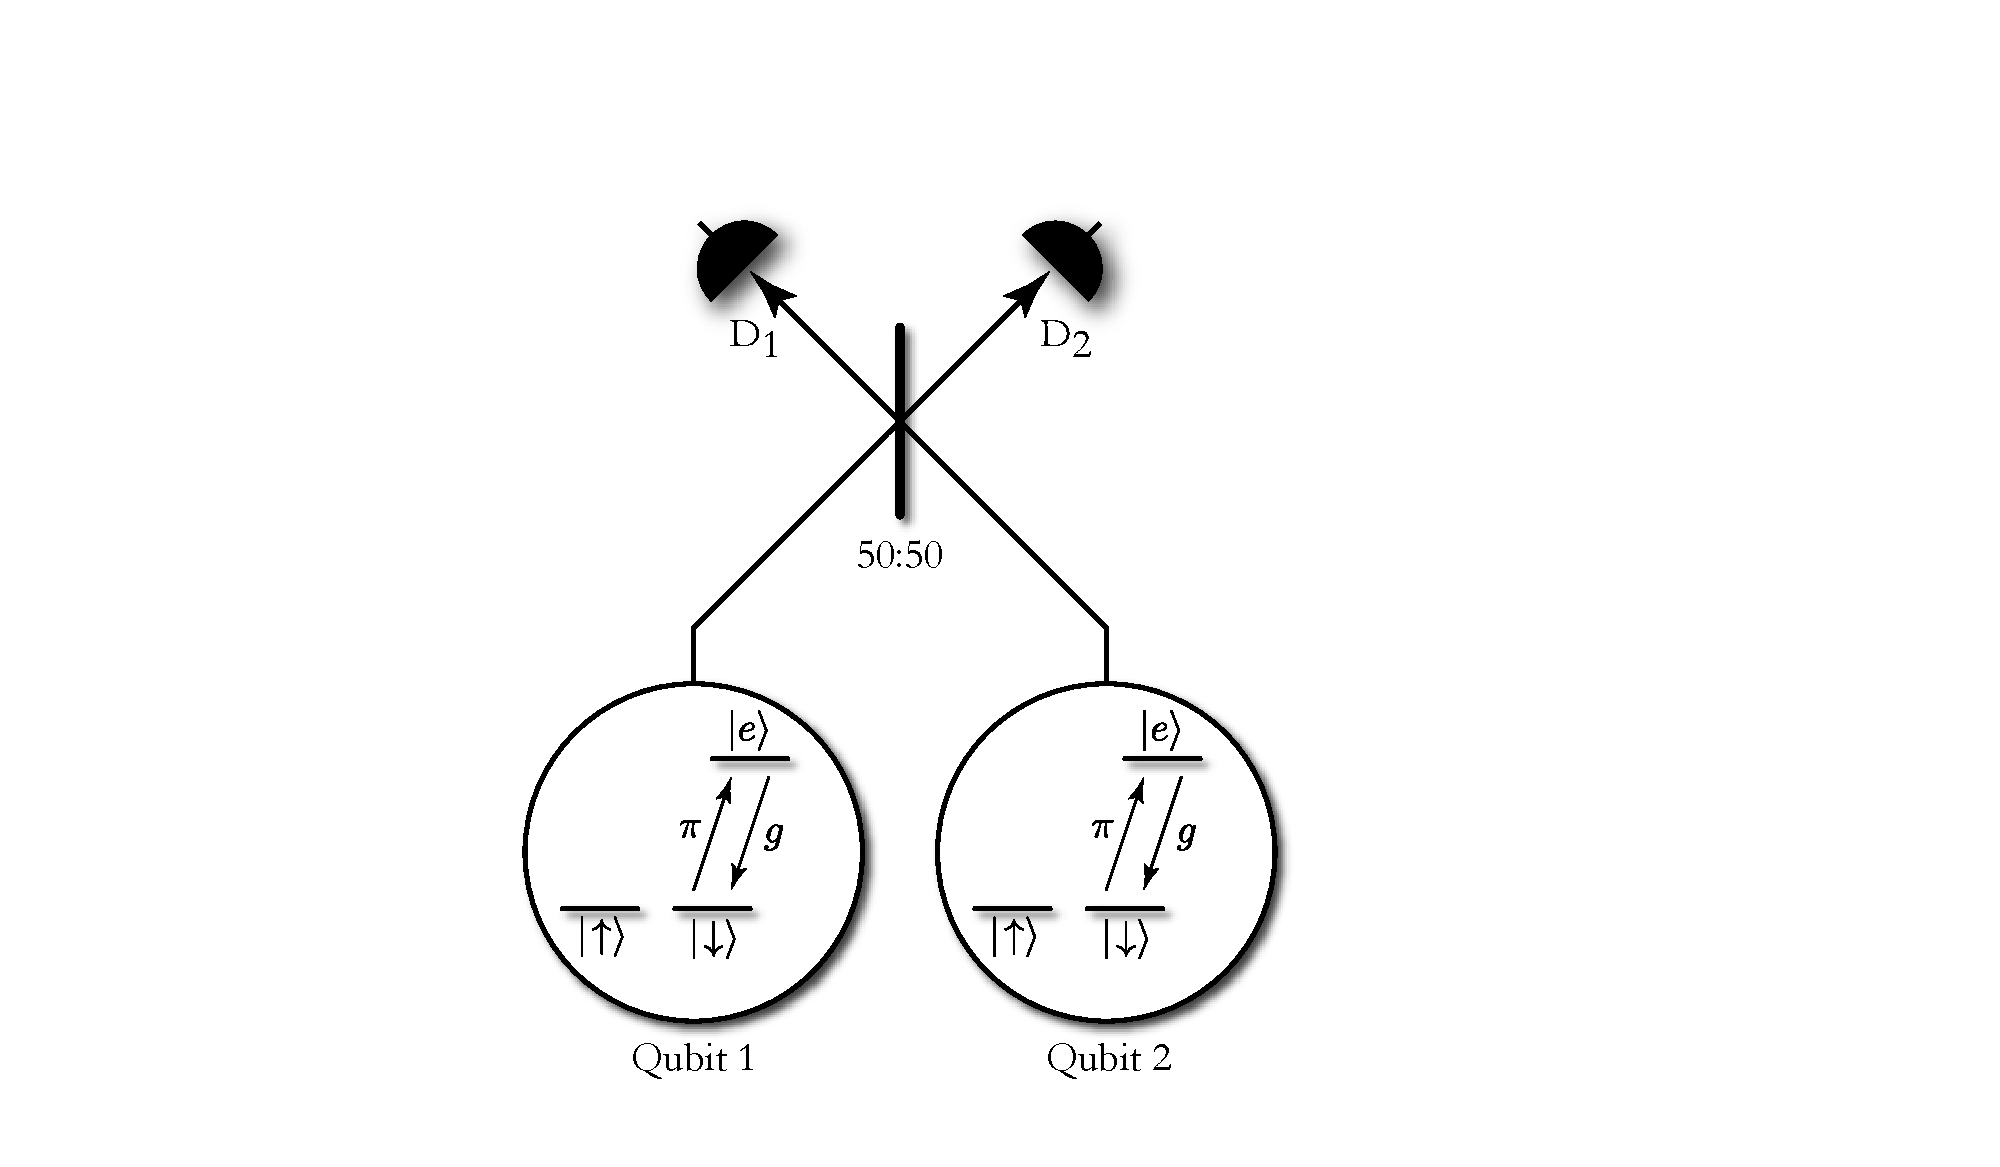
\includegraphics[clip=true, width=0.475\textwidth]{barrett_kok}
\captionspacefig \caption{Two atomic systems in $\lambda$-configurations, each coupled with an optical mode. An EO between them is mediated via linear optics which-path erasure. Each system contains two degenerate ground states, which jointly encode a qubit (\mbox{$\ket{0}\equiv\ket{\!\uparrow}$}, \mbox{$\ket{1}\equiv\ket{\!\downarrow}$}), and an additional excited state ($\ket{e}$), which only couples to the $\ket{\!\downarrow}$ state. A $\pi$-pulse excites the electron from the $\ket{\!\downarrow}$ to the $\ket{e}$ state, after which emission of a photon is associated with a coherent relaxation back to $\ket{\!\downarrow}$. If the two optical modes are interfered on a 50:50 beamsplitter, and a single photon is detected between the two photo-detectors, $D_1$ and $D_2$, the two emission processes become indistinguishable, and which-path erasure entangles the two qubits by projecting them onto a maximally entangled Bell pair. More complicated networks based on this EO allow the preparation of cluster states, enabling universal quantum computation. In a quantum networking context, the matter qubits could be held by a client, and the optical interferometry implementing the computation outsourced to the cloud, i.e the PBS, $D_1$ and $D_2$ are implemented in the cloud. This would also facilitate the preparation of shared entangled states, where different clients possess parts of an entangled state, potentially physically separated over long distances.} \label{fig:barrett_kok}
\end{figure}

The attractive feature of this type of approach is that the actual entanglement is generated using all-optical operations, despite the underlying logical qubits being stationary and potentially physically separated a long distance apart, mitigating the need for direct matter-matter interactions, and enabling distributed computation. Optical interfacing is discussed in Sec.~\ref{sec:opt_inter}. This allows the EOs to be performed remotely in the cloud, without physically moving the stationary qubits. Such hybrid systems present an interesting platform for cloud quantum computing -- despite the qubits being stationary, we are able to outsource the interactions between them to distant servers or even satellites.

Importantly, the beamsplitter mediating the which-path erasure EO is based upon HOM interference, and therefore does not require interferometric stability, making the outsourcing process relatively robust and suitable for long-range operation.

This protocol can be regarded as a variation on the entanglement swapping protocol (Sec.~\ref{sec:swapping}), whereby entanglement between matter qubits and optical modes is swapped onto entanglement between the distinct matter qubits.

Alternately, if there is no direct line of quantum communication between two qubits, an EO can be performed by directly employing the same idea in reverse. We imagine that a third party, such as a satellite, acts as a server for entangled Bell pairs. Two parties receive one qubit each from the pair. Then they perform an EO between their halves of the Bell pair and their local qubits. With appropriate local corrections, mediated by only cheap classical communication, this teleports the action of an EO onto the two qubits, creating a link between them.

Expanding upon this idea, we can envisage distributed models for quantum computation, where the qubits needn't even be of the same physical medium. We could, for example, entangle quantum dot qubits, atomic qubits, and atomic ensemble qubits with one another by coupling them to optical modes and performing which-path erasure between them. This enables distributed quantum computation between hosts possessing quantum infrastructure comprising different physical mediums (provided the photons emitted by those systems may be made indistinguishable, such that HOM interference is possible).

\begin{table}[!htbp]
\begin{mdframed}[innertopmargin=3pt, innerbottommargin=3pt, nobreak]
\texttt{
function WhichPathErasure():
\begin{enumerate}
\item Alice and Bob each prepare an equal superposition of the two logical basis states,
\begin{align}
\ket\psi_\mathrm{in} = &\frac{1}{2}(\ket{\!\uparrow}_{A_1}+\ket{\!\downarrow}_{A_1})\ket{0}_{A_2}\nonumber \\
&\cdot (\ket{\!\uparrow}_{B_1}+\ket{\!\downarrow}_{B_1})\ket{0}_{B_2},
\end{align}
where $A_1/B_1$ denote the matter qubits, and $A_2/B_2$ denote their coupled optical modes.
\item Apply a $\pi$-pulse to each qubit, inducing a \mbox{$\ket{\!\downarrow}\to\ket{e}$} transition,
\begin{align}
\ket\psi_\pi = \hat{U}_\pi\ket\psi_\mathrm{in} = &\frac{1}{2}(\ket{\!\uparrow}_{A_1}+\ket{e}_{A_1})\ket{0}_{A_2}\nonumber \\
&\cdot (\ket{\!\uparrow}_{B_1}+\ket{e}_{B_1})\ket{0}_{B_2}.
\end{align}
\item Wait for a coherent relaxation, inducing the transition \mbox{$\ket{e}\to\ket{\!\downarrow}\hat{a}^\dag$}, which emits a single photon,
\begin{align}
\ket\psi_\mathrm{relax} = \hat{U}_\mathrm{relax}\ket\psi_\pi = &\frac{1}{2}(\ket{\!\uparrow}_{A_1}+\ket{\!\downarrow}_{A_1}\hat{a}^\dag_{A_2})\ket{0}_{A_2}\nonumber \\
&\cdot (\ket{\!\uparrow}_{B_1}+\ket{\!\downarrow}_{B_1}\hat{a}^\dag_{B_2})\ket{0}_{B_2}.
\end{align}
\item Apply a 50:50 beamsplitter between the two optical modes,
\begin{align}
\ket\psi_\mathrm{BS} = \hat{U}_\mathrm{BS} \ket\psi_\mathrm{relax} = &\frac{1}{2}(\ket{\!\uparrow}_{A_1}+\ket{\!\downarrow}_{A_1}[\hat{a}^\dag_{A_2}+\hat{a}^\dag_{B_2}])\nonumber \\
&\cdot (\ket{\!\uparrow}_{B_1}+\ket{\!\downarrow}_{B_1}[\hat{a}^\dag_{A_2}-\hat{a}^\dag_{B_2}])\nonumber \\
&\cdot \ket{0}_{A_2}\ket{0}_{B_2}.
\end{align}
\item Conditional upon detecting exactly one photon between the output optical modes, we obtain,
\begin{align}
\ket\psi_\mathrm{out}^{1,0} = \bra{1,0}_{A_2,B_2} \ket\psi_\mathrm{BS} = \frac{1}{2} (\ket{\!\uparrow,\downarrow}_{A_1,B_1} + \ket{\!\downarrow,\uparrow}_{A_1,B_1}), \nonumber \\
\ket\psi_\mathrm{out}^{0,1} = \bra{0,1}_{A_2,B_2} \ket\psi_\mathrm{BS} = \frac{1}{2} (\ket{\!\uparrow,\downarrow}_{A_1,B_1} - \ket{\!\downarrow,\uparrow}_{A_1,B_1}),
\end{align}
which is a Bell pair between the matter qubits.
    \item $\Box$
\end{enumerate}}
\end{mdframed}
\captionspacealg \caption{Using which-path erasure to entangle two $\lambda$-configuration matter qubits via post-selected linear optics. Note that the two matter qubits could in principle be arbitrarily physically separated. Only the emitted photons need be brought together locally for the implementation of a beamsplitter operation. This lends such entanglement generation protocols to distributed implementation.} \label{alg:which_path}
\end{table}

%
% Atomic Ensembles
%

\subsection{Atomic ensembles}

\comment{To do}

%
% Ion Traps
%

\subsection{Ion traps}\index{Ion traps}

\comment{To do. Talk about optical interfacing.}

%
% Artificial Atoms
%

\subsection{Superconducting circuits}\index{Superconductors!Circuits}\label{sec:artificial_atoms}

Qubits may be engineered by considering the lowest two energy levels of a quantum system. Based on the spacing between their energy levels, such quantum systems are classified into two categories:
\begin{itemize}
	\item Quantum harmonic oscillator type: have equal spacing between energy levels.\index{Quantum harmonic oscillators}
	\item Atomic type: have unequal spacing between energy levels.\index{Artificial atoms}
\end{itemize}
We illustrate these two cases in Fig.~\ref{fig:artificial_atom_energy_levels}, with their corresponding energy level diagrams. The energy levels of these two classes of systems obey,
\begin{align}
E_{n} &= \hbar \omega \left(n+\frac{1}{2}\right) \quad (\mathrm{Oscillator\,levels}), \nonumber \\ 
E_{n} &= -\frac{E_{0}}{n^{2}} \quad (\mathrm{Atomic\,levels}),
\end{align}
where \mbox{$n\in\mathbb{Z}^+$} denotes the discrete energy level, $\omega$ is optical frequency, and $E_0$ is the lowest-lying ground state energy\index{Ground states}.

\begin{figure}[!htbp]
\includegraphics[clip=true, width=0.475\textwidth]{artificial_atom_energy_levels}
\captionspacefig \caption{The energy levels of: (a) a quantum oscillator; and, (b) an atomic system. The quantum oscillator exhibits equidistant separation between energy levels, whereas for the atomic system the energy levels are non-uniform.}\label{fig:artificial_atom_energy_levels}\index{Energy levels}
\end{figure}

To construct a qubit we should be able to use external fields\index{Control fields} to control and selectively drive transitions between only two energy levels in the system. Such a procedure is easy to achieve in atomic systems, but it is not possible to address only two levels in a quantum oscillator due to the harmonicity\index{Harmonicity} (equal energy spacing) between energy levels. On the other hand, it's hard to work with individual natural atoms, mainly because of their size, which makes their individual isolation and control very challenging. To overcome this problem, we need to develop new quantum devices with anharmonic\index{Anharmonicity} energy spectra\index{Energy spectra}. Such devices are referred to as \textit{artificial atoms}\index{Artificial atoms}, due to their similarity to natural atoms in the anharmonicity of their energy level spectrum.

One of the most widely used types of artificial atom are superconducting qubits \cite{bib:martinis1985energy, bib:shnirman1997quantum, bib:averin1998adiabatic, bib:devoret2004superconducting, bib:makhlin2001quantum}\index{Superconductors!Qubits}, a class of non-linear quantum circuits\index{Non-linear quantum circuits}. An LC oscillator\index{LC oscillator} composed of an inductor $L$\index{Inductors} and capacitance $C$\index{Capacitors} is a typical example of a linear quantum circuit\index{Linear quantum circuits} with equal spacing. By introducing a Josephson junction\index{Josephson junction} into the linear quantum circuit we can make it non-linear, with anharmonic energy spectrum.

A Josephson junction \cite{bib:josephson1974the} comprises two bulk superconducting materials\index{Superconductors}, separated by a thin layer of insulating material\index{Insulators}. In the superconducting phase the superconductors contain Cooper-pairs\index{Cooper-pairs}, composed of paired electrons. These Cooper-pairs move from one superconducting layer to another through the insulating layer via quantum tunnelling\index{Tunnelling}. The quantum mechanical nature of Josephson junctions is determined by two important energy scales:
\begin{itemize}
\item Josephson coupling energy, $E_{J}$.\index{Josephson coupling energy}
\item Coulomb energy, $E_C$.\index{Coulomb energy}
\end{itemize}
The ratio between these two energy scales determines the energy spectrum of the superconducting qubit. This yields three distinct types of qubits:
\begin{itemize}
\item Voltage-driven charge qubits \cite{bib:bouchiat1998quantum, bib:nakamura1999coherent}.\index{Charge qubits}
	\item Flux-driven flux qubits \cite{bib:friedman2000quantum, bib:van2000quantum}.\index{Flux qubits}
	\item Current-driven phase qubits \cite{bib:martinis2002rabi}.\index{Phase qubits}
\end{itemize} 
These circuits and energy level diagrams for these are illustrated in Fig.~\ref{fig:superconductor_circuits}.

\begin{figure}[!htbp]
\includegraphics[clip=true, width=0.475\textwidth]{superconducting_qubits}
\captionspacefig \caption{Simplified circuits of the different kinds of superconducting qubits, namely the charge qubit, flux qubit and phase qubit. Below each circuit are their respective energy level diagrams.}\label{fig:superconductor_circuits}
\end{figure}

\subsubsection{Charge qubits}\index{Charge qubits}

A non-linear quantum circuit driven by voltage\index{Voltage} is referred to as a charge qubit, whose Hamiltonian takes the form,
\begin{align}
\hat{H} = \frac{\hat{q}^{2}}{2C} - E_{J} \cos \left( \frac{2e}{\hbar} \hat\phi \right).
\label{circuitHamiltonian}
\end{align}
Here $\hat{q}$ is the charge in the superconducting system and $\hat\phi$ is flux\index{Flux}. The total capacitance of the circuit is given by $C$, and $E_{J}$ is the Josephson energy\index{Josephson energy}. The Hamiltonian in Eq.~(\ref{circuitHamiltonian}) can be rewritten as,
\begin{align}\label{eq:charge_qubit_hamiltonian}
\hat{H} = 4E_C (\hat{n} - n_{g})^{2} - E_{J} \cos (\hat{\phi}) .
\end{align}
The variables $\hat{q}$ and $\hat{\phi}$ are canonically conjugate\index{Canonically conjugate} and satisfy the commutation relation,
\begin{align}
[ \hat{\phi},\hat{q} ] = i \hbar.
\end{align}
In a truncated charge basis the Hamiltonian is,
\begin{align}
\hat{H} &= 4 E_C \sum_{n = -N}^{N} (\hat{n} - n_{g})^{2} \ket{n}\bra{n}\nonumber\\
&- E_{J} \sum_{n = -N}^{N-1} \ket{n+1}\bra{n} + \ket{n}\bra{n+1}.
\end{align}

The energy eigenstates are the charge states\index{Charge states} $\ket{n}$, hence these qubits are referred to as charge qubits. In general the charge qubit \cite{bib:bouchiat1998quantum, bib:nakamura1999coherent} is operated in the region,
\begin{align}
	\frac{E_J}{E_C} \approx 1.
\end{align}

Charge qubits are highly sensitive to noise except at particular working points referred to as `sweet spots'\index{Sweet spots}. But it is experimentally difficult to control the voltage and current such that the qubit is maintained at these desired working conditions.

To overcome this, a special design of charge qubit known as the \textit{transmission line shunted plasma oscillation qubit} or `transmon' \cite{bib:koch2007charge}\index{Transmon} with,
\begin{align}
\frac{E_J}{E_C} \gg 1,
\end{align}
was suggested. The transmon is highly robust against external noise compared to the charge qubit. But the energy levels become more and more harmonic\index{Harmonicity} (i.e equally spaced) as we move away from the region,
\begin{align}
	\frac{E_{J}}{E_{C}} \approx 1.
\end{align}
Thus the charge qubits are designed by giving consideration to the trade-off between robustness against external noise and the anharmonicity\index{Anharmonicity} between the levels. A 20-qubit prototype quantum computer developed by IBM\index{IBM} employs transmon-type superconducting qubits \cite{bib:gambetta2017building}. 

\subsubsection{Flux qubits}\index{Flux qubits}

The flux qubit is popularly known as the RF SQUID (Radio Frequency Superconducting QUantum Interference Device)\index{SQUIDs}, which uses an AC current\index{Alternating current}. This qubit can be considered as the magnetic analogue of the charge qubit. In a charge qubit the Josephson junction is driven by a capacitor, but in a flux qubit, a superconducting transformer\index{Superconductors!Transformers} circuit generates the flux which drives the circuit. The Hamiltonian of the circuit is,
\begin{align}
\hat{H} = \frac{\hat{q}^{2}}{2 C_{J}} + \frac{\hat\phi^{2}}{2 L} - E_{J} \cos \left( \frac{2e}{\hbar}(\hat\phi - \phi_\mathrm{ext}) \right).
\end{align}

Here we can observe that there are three energy scales namely,
\begin{align}
E_J,& \nonumber\\
E_{C} &= \frac{2e^{2}}{C},\nonumber\\
E_{L} &= \frac{{\phi_{0}}^{2}}{2L}.
\end{align}
The quantum properties of the qubits depend on the interplay between these parameters. The Cooper-pairs in a flux qubit are confined to a double well potential\index{Double well potential}. The variables $Q$ and the total magnetic flux $\Phi$\index{Magnetic flux} are the conjugate variables, satisfying the commutation relation,
\begin{align}
[\hat{Q},\hat\Phi] = i \hbar.
\end{align}

Flux qubits are very robust against charge noise \cite{bib:you2005fast}, and hence have very long decoherence times\index{Decoherence!Times}, making them one of the most attractive qubit candidates for the construction of quantum computers. The early quantum computing devices developed by D-Wave\index{D-Wave} employ flux qubits \cite{bib:harris2018phase}.

\subsubsection{Phase qubits}\index{Phase qubits}

Current-driven superconducting qubits are referred to as phase qubits \cite{bib:martinis2002rabi}. They are commonly known as DC SQUIDs, and operate in the regime of very high values of $E_{J}/E_{C}$.

The Hamiltonian of a phase qubit is,
\begin{align}
\hat{H} = E_{C} \hat{p}^{2} - I \phi_{0} \hat\delta - I_{0} \phi_{0} \cos \hat\delta,
\label{eq:phase_qubit_hamiltonian}
\end{align}
where $\hat\delta$ is the gauge invariant\index{Gauge invariance} phase-difference operator\index{Phase-difference operator} and the charge on the capacitor is $2pe$. These operators are conjugate variables, satisfying the commutation relation,
\begin{align}
	[\hat\delta, \hat{p}] = i \hbar.
\end{align}

In the phase qubit, Cooper-pairs\index{Cooper-pairs} experience a washboard potential\index{Washboard potential}. Since their decoherence times\index{Decoherence!Times} are very small compared to flux and charge qubits, they are not that widely employed.

\subsubsection{Quantum gates}\index{Quantum gates}

To build useful quantum information processing devices, we require quantum gates to act upon our superconducting qubits. This is a field under active development \cite{bib:blais2004cavity, bib:chow2011simple, bib:chow2013microwave}. Below we provide a brief description of the operation of single- and two-qubit quantum gates based on superconducting qubits.

\paragraph{Single-qubit gates}

A single superconducting qubit, which is coherently controlled using microwaves, can be used as a quantum gate. Let us consider a cavity with resonant frequency $\omega_{r}$\index{Resonant frequency} and drive frequency $\omega_{d}$\index{Drive frequency}, where the difference \mbox{$\Delta_{r} = \omega_{r} - \omega_{d}$} is the detuning\index{Detuning} between the cavity and the drive. When \mbox{$\omega_{d} \approx \omega_{r}$} one can read the state of a superconducting qubit using microwaves. But when \mbox{$\omega_{d} = \omega_{q} \ll \omega_{r}$} the microwave can be used to perform gate operations on the qubit without measuring its state.

A system comprising a superconducting qubit and a microwave can be described using the Jaynes-Cummings Hamiltonian\index{Jaynes-Cummings Hamiltonian},
\begin{align}
\hat{H} = \Delta _{r} \hat{a}^{\dag} \hat{a} - \frac{\Delta_{q}}{2} \hat\sigma_{z} + g (\hat{a}^{\dag} \hat\sigma_{-} + \hat{a} \hat\sigma_{+}) + \xi(t) (\hat{a}^{\dag} + \hat{a}),
\label{eq:driven_jc_hamiltonian}
\end{align}
where $\hat{a}^{\dag}$ ($\hat{a}$) is the creation (annihilation) operator corresponding to the microwave photon, and $\sigma_{+}$ ($\sigma_{-}$) is the spin raising (lowering) operator\index{Spin operators}. The factors \mbox{$\Delta_{r} = \omega_{r} - \omega_{d}$} and \mbox{$\Delta_{q} = \omega_{q} - \omega_{d}$} are the detuning parameters\index{Detuning}. The factor $g$ is the coupling between the microwave photon and the qubit, and $\xi(t)$ is the envelope\index{Envelope} of the microwave pulse. The effective Hamiltonian is,
\begin{align}
\hat{H}_\mathrm{eff} &= \left( \Delta_{r} + \frac{g^{2}}{\Delta} \hat\sigma_{z} \right) \hat{a}^{\dag} a - \frac{1}{2} \left(\Delta_{q} - \frac{g^{2}}{\Delta} \right) \hat\sigma_{z} \nonumber\\
&+ \xi(t) (\hat{a}^{\dag} + \hat{a}) - \frac{g \xi(t)}{\Delta} \hat\sigma_{x}.
\end{align}

To perform an $X$-gate, we choose a drive frequency\index{Drive frequency},
\begin{align}
\omega_{d} = \omega_{q} - \frac{g^{2}}{\Delta}(2 \bar{n} + 1),
\end{align}
which causes the $\sigma_{z}$ term to disappear, leaving us with a pure $\sigma_{x}$ rotation. Using a phase-shifted drive,
\begin{align}
H_{d}(t) = \xi(t) i (\hat{a}^{\dag} - \hat{a}),
\end{align}
one might obtain a pure $\sigma_{y}$ rotation, yielding a $Y$-gate. Finally we note that using a drive,
\begin{align}
	\omega_{d} = \omega_{q} - \frac{g^{2}}{\Delta}(2 \bar{n} + 1) - 2 \xi(t)\frac{g}{\Delta},
\end{align}
we may construct a Hadamard gate. 

\paragraph{Two-qubit gates}

Quantum gates operating on two qubits can be realised in many different ways. But in terms of their construction and operation, they can be divided into two classes. In the first class of quantum gates the superconducting qubits can be tuned over a wide range of frequencies. A good example of this is the iSWAP gate\index{iSWAP gate}, in which two Cooper-pair\index{Cooper-pairs} boxes are coupled via a transmission line resonator\index{Transmission line resonator}. In the rotating frame of reference\index{Rotating frame}, the effective Hamiltonian of the system is,
\begin{align}
\hat{H}_\mathrm{eff} &= \frac{g^{2}}{\Delta} \left( \hat{a}^{\dag} \hat{a} + \frac{1}{2} \right) (\hat\sigma_{z,1} + \hat\sigma_{z,2}) \nonumber\\
&- \frac{g^{2}}{\Delta} (\hat\sigma_{+,1} \hat\sigma_{-,2} + \hat\sigma_{+,2} \hat\sigma_{-,1}).
\end{align}

The parameters of the two qubits can be adjusted by tuning their flux. The interaction between qubits can be turned on and off by tuning the qubits in and out of resonance with one another. The advantage of the first class of quantum gates is that they can be operated in a region where the frequency of the two qubits differ from one another and the interaction between them is very strong. But the disadvantage is that they are sensitive to flux noise, hence requiring extra flux bias lines for tuning them properly.

The second class of quantum gates is built up of superconducting qubits with fixed frequencies, driven by microwaves. The cross-resonance gate\index{Cross-resonance gate}, the bSWAP\index{bSWAP gate} or Bell pairRabi gate\index{Bell pairRabi gate}, and the MAP gate\index{MAP gate} belong to this class. The effective Hamiltonian of the cross-resonance gate is,
\begin{align}
\hat{H}_\mathrm{eff} = - \left( \frac{\tilde{\omega}_{1} - \tilde{\omega}_2}{2} \right) \hat\sigma_{z,1} + \frac{\Omega(t)}{2} \left(\hat\sigma_{x,1} - \frac{J}{\Delta_{12}} \hat\sigma_{z,1} \hat\sigma_{x,2} \right),
\end{align}
where,
\begin{align}
	\tilde{\omega}_{1} &= \omega_{1} + \frac{J^{2}}{\Delta_{12}}, \nonumber\\
		\tilde{\omega}_{2} &= \omega_{2} - \frac{J^{2}}{\Delta_{12}}, \nonumber\\
\Delta &= \omega_{1} -\omega_{2}.		
\end{align}
The factors $\omega_{1}$ and $\omega_{2}$ are the frequencies of the first and second qubits, and $\Delta_{12}$ is the detuning\index{Detuning}. The first qubit is rotating with frequency $\frac{1}{2}(\tilde{\omega_{1}} - \tilde{\omega_{2}})$ around the $Z$-axis, with a little shift in the $X$-direction, yielding an $X$-gate. Similarly we can construct a microwave-activated CZ (MAP) gate\index{MAP gate} using two transmons. The system of two transmons is modelled using a system of two coupled Duffing oscillators\index{Duffing oscillators}. The effective Hamiltonian in the two qubit space reads,
\begin{align}
\hat{H}_\mathrm{eff} &= - \frac{1}{2} \left( \omega_{01} - \frac{\zeta}{2} \right) \hat\sigma_{z,1} - \frac{1}{2} \left( \omega_{10} - \frac{\zeta}{2} \right) \hat\sigma_{z,2} \nonumber\\
&+ \frac{\zeta}{4} \hat\sigma_{z,1} \hat\sigma_{z,2}. 
\end{align}

Through this Hamiltonian we can realise a CZ gate, with gate time $514$ns and high fidelity. The second class of quantum gates have a longer coherence time\index{Coherence time}, since the superconducting qubits can be parked at the sweet spots\index{Sweet spots} of coherence where the effects of noise on the qubits are less substantial. But, control of the qubits is much harder, since we need to maintain them with the same qubit parameters for an extended period of time.

%
% Adiabatic Quantum Computing & Quantum Annealing
%

\subsection{Adiabatic quantum computing \& quantum annealing}\index{Adiabatic quantum computation}\index{Quantum annealing}

\comment{To do. Talk about optical interfacing.}


\latinquote{Acta deos numquam mortalia fallunt.}

\sketch{sketch_9}

%
% Cloud quantum computing
%

\part{Cloud quantum computing}\label{part:cloud_QC}\index{Cloud quantum computing}

%
% The Quantum Cloud
%

\section{The Quantum Cloud} \label{sec:cloud} 
\index{Cloud quantum computing}

From the perspective of quantum computing, by far the most pressing goal for quantum networking is to facilitate \textit{cloud quantum computing}, whereby computations can be performed over a network via a client/server model. This will be of immense importance economically, allowing very expensive quantum computers to be accessible to end-users, who otherwise would have been priced out of the market. This economic model is critical to the early widespread adoption of quantum computation.

There are several protocols necessary to facilitate cloud quantum computing. First of all, we must have a means by which to remotely process data prepared by a host on a server(s). At the most basic level, this simply involves communicating quantum and/or classical data from a client to a single server for processing, which returns quantum or classical information to the client. In the most general case, a computation may be processed by multiple servers, each responsible for a different part of the computation -- \textit{distributed quantum computation}.

Many real-world applications for quantum computing will involve sensitive data, in terms of both the information being processed and the algorithms being employed. This necessitates encryption protocols allowing computations to be performed securely over a network, such that intercept-resend attacks are unable to infer the client's data, and even the host itself is unable to do so -- \textit{homomorphic encryption} and \textit{blind quantum computing}. These form the basic building blocks from which a secure cloud-based model for quantum computing may be constructed, and economic models based on the outsourcing of computations may emerge.

\comment{Latin quote}\index{Latin}

%
% Outsourced Quantum Computation
%

\subsection{Outsourced quantum computation} \index{Outsourced quantum computation}

Most simply, an outsourced computation involves Alice preparing either a quantum or classical input state, which she would like processed on Bob's computer. Bob performs the computation and returns either a quantum or classical state to Alice.

The algorithm, which Bob implements, could either be stipulated by Alice, in which case she is purely licensing Bob's hardware, or by Bob, in which case she is licensing his hardware and software. In the case of classical input and classical output, such an outsourced computation is trivial from a networking perspective, requiring no usage of the quantum network whatsoever. In the case of quantum input and/or output data, the quantum network will be required.

Despite the model being very simple, there may still be stringent requirements on the costs in the network. When the result of the computation is returned to Alice, there may be fidelity requirements. An approximate solution to a problem, or a computation with any logical errors whatsoever, may be useless, particularly for algorithms, which are not efficiently verifiable. For example, if Alice is attempting to factorise a large number using Shor's algorithm\index{Shor's algorithm}, a number of incorrect digits may make the the correct solution effectively impossible to determine. Or if a large satisfiability problem is being solved, almost any classical bit-flip errors will invalidate the result, requiring additional computation by Alice to resolve (which may be exponentially complex to perform).

In the case of classical communication of input and output data, we can reasonably assume error-free communication, owing to its digital nature. However, in the case of quantum communication it is inevitable that at least some degree of noise will be present. Depending on the application, this may require the client and host to jointly implement a distributed implementation of QEC (Secs.~\ref{sec:QOS} \& \ref{sec:topol_codes}), whereby Alice and Bob communicate encoded states with one another, to which syndrome measurement and error correction are applied upon receipt. This will necessitate a limited amount of quantum processing to be directly available to Alice. In the case where she is completely starved of any quantum processing resources whatsoever, this may be a limiting factor. Otherwise, this type of cooperative QEC may be plausible.

%
% Distributed Quantum Computation
%

\subsection{Distributed quantum computation} \label{sec:dist_QC} \index{Distributed quantum computation}

The elementary model described above is very limited, as many realistic data processing applications will require multiple stages of computations to be performed, potentially by different hosts. For example, a client may need data processed using multiple proprietary algorithms owned by different hosts, and the processing will need to be distributed across the network \cite{bib:Cirac99}.

There are two main models for how a distributed computation may proceed -- in \textit{parallel}, or in \textit{series} -- whereby sub-algorithms are performed either side-by-side simultaneously, or one after another in a pipeline. The two models are illustrated in Fig.~\ref{fig:distributed}.

\begin{figure}[!htb]
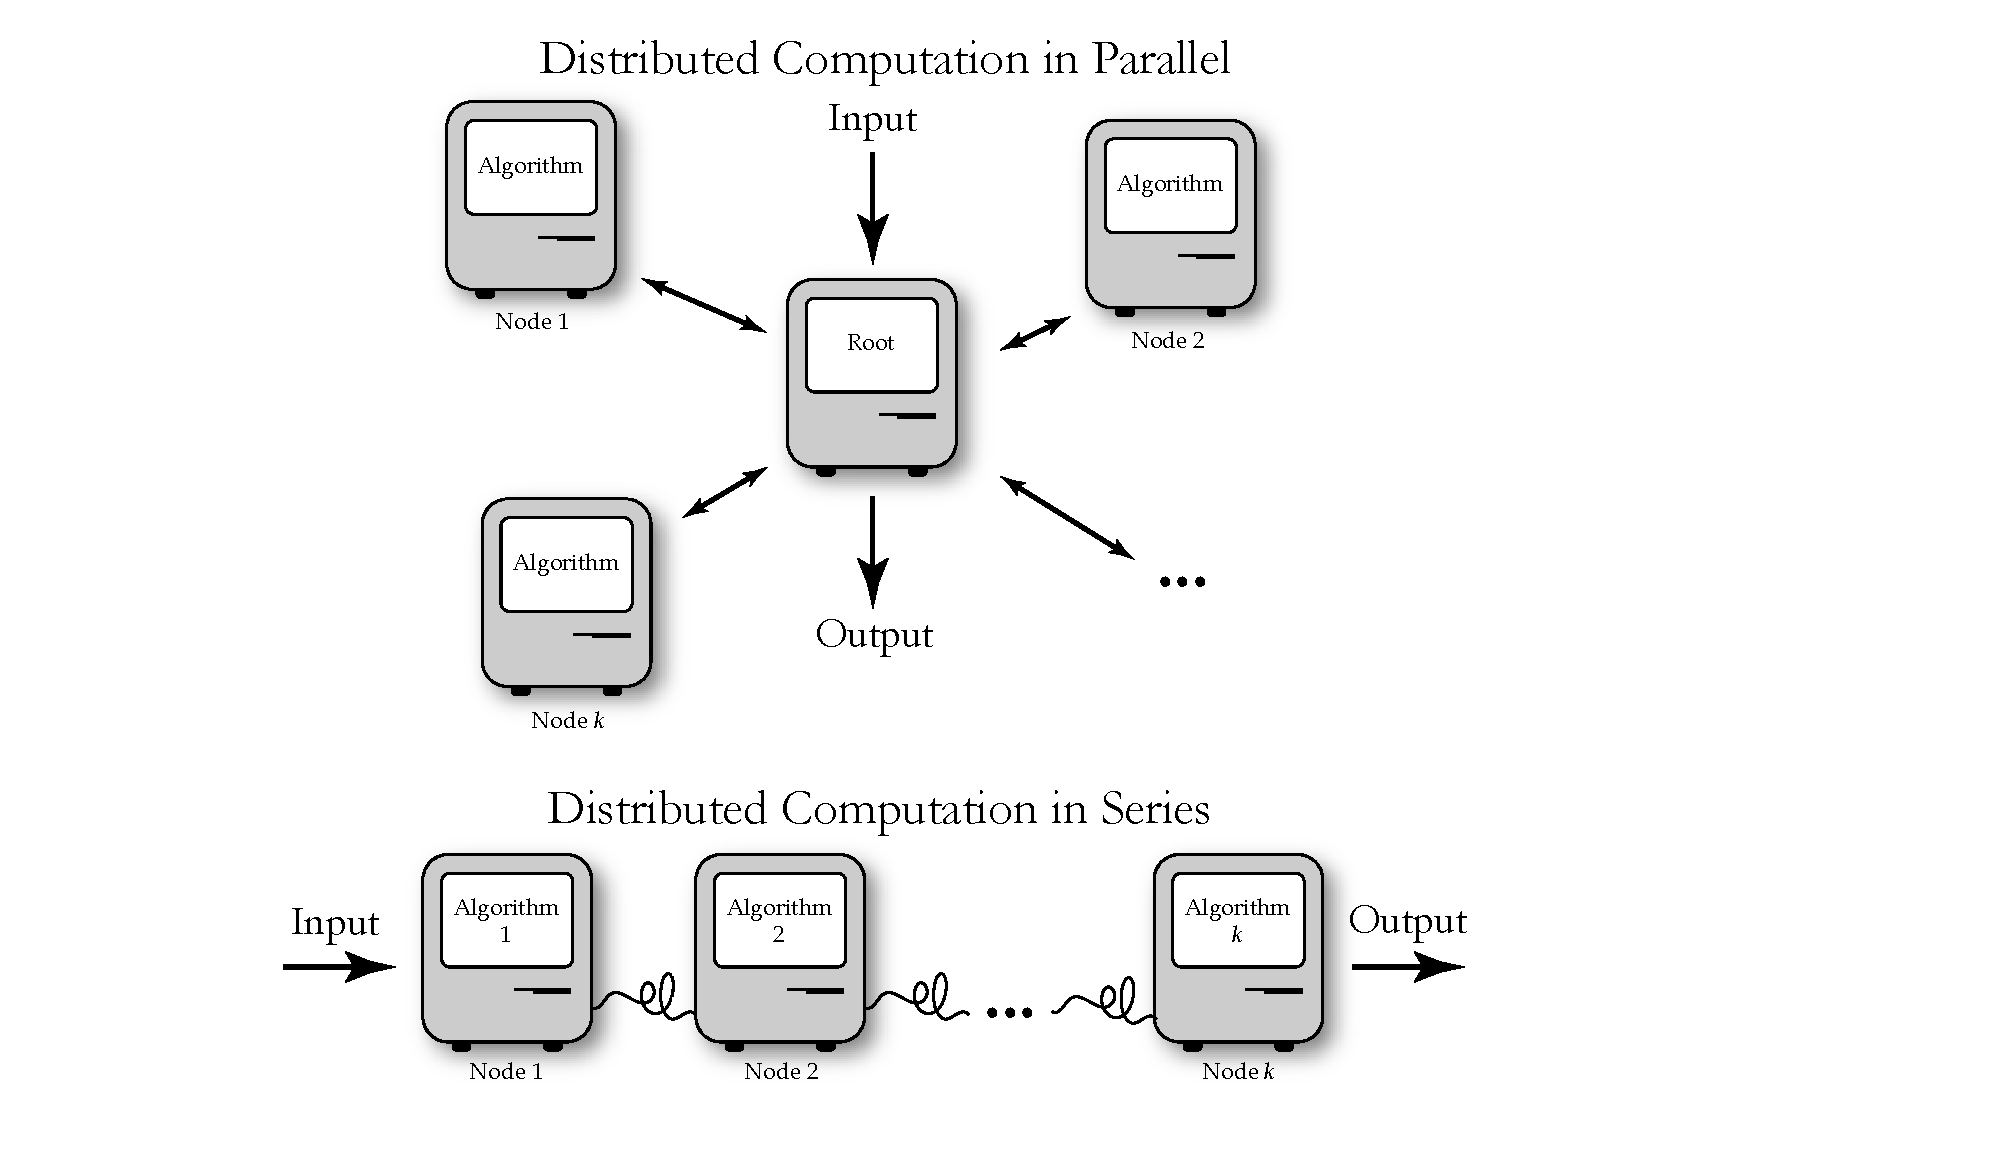
\includegraphics[width=0.47\textwidth]{distributed}
\caption{Models for distributed computation in parallel and in series. In parallel, a root node oversees the total computation, delegating tasks to child nodes, which process data independently of one another. In series the nodes sequentially process data in a pipeline of algorithmic stages.} \label{fig:distributed}
\end{figure}

Classical parallel processing typically involves a root node, which delegates tasks to be performed in parallel by a number of child nodes, and the results returned to the root node, which potentially applies an algorithm to merge the set of results, before returning a final result to the client. Classical models such as Google's \textsc{MapReduce} protocol \cite{bib:MapReduce}\index{MapReduce} are built on this idea.

In classical computing, parallel processing is widely employed to shorten algorithmic runtimes. However, the increase in clock-cycles scales only linearly with the number of nodes in the network: $k$-fold parallelisation yields a \mbox{$\sim k$}-fold speedup. For time-critical applications, such a linear improvement may be already highly beneficial, albeit costly. The attractive feature of quantum computing, however, is the potentially exponential improvement in algorithmic performance of certain tasks over their classical counterparts. This exponential relationship implies that parallelisation in general no longer has a simple linear tradeoff.

Let $t_c$ be the time required by a classical algorithm to solve a given problem, and $t_q$ the time required to solve the same problem using a quantum algorithm. In the case of algorithms exhibiting exponential quantum speedup, we will have,
\begin{align}
t_c = O(\text{exp}(t_q)).
\end{align}
If we now increase the quantum processing power $k$-fold, the equivalent classical processing time is (in the best case),
\begin{align}
t_c' &= O(\text{exp}(t_q k)) \nonumber \\
&= O(\text{exp}(t_q)^{k}) \nonumber \\
&= O({t_c}^{k}).
\end{align}
Thus, $k$-fold quantum enhancement corresponds to a $k$th-order exponential enhancement in the equivalent classical processing time, which clearly scales much more favourably than the linear $k$-fold enhancement offered by classical parallelisation.

The alternate scenario is in-series distributed computation, in which a computation proceeds through a pipeline of different stages, potentially performed by different hosts. This model allows a complex algorithm comprising smaller subroutines, each of which may be proprietary with different owners, to be delegated across the network. The different stages may communicate classical and/or quantum data. As with the simple single-host model, if the different stages of the processing pipeline are sharing quantum data, distributed QEC will generally be necessary to protect the computation in transit. This necessarily introduces an (efficient) overhead in the number of physical qubits being communicated across the network, introducing additional bandwidth costs, which must be accommodated for in networking strategies.

The cluster state (Sec.~\ref{sec:CSQC}), topological code (Sec.~\ref{sec:topol_codes}) and quantum random walk (Sec.~\ref{sec:QW}) models for quantum computation may find themselves to be particularly well-suited to distributed implementation, since they naturally reside on graphs, whose nodes needn't be held locally by a single user, but could instead be shared across multiple hosts with the ability for graph nodes to intercommunicate. Then only classical communication is required to complete a computation will quantum information not localised to any particular node.

Additionally, the entangling gates which build cluster states all commute and may be implemented simultaneously in parallel. This enables a distributed cluster state to be constructed in a `patchwork' fashion, as shown in Fig.~\ref{fig:patchwork_cluster}. Now the computation is truly distributed in the sense that the computation resides collectively across the distributed cluster state, held by any number of users.

This approach overlaps with the modularised approach for quantum computation discussed in the upcoming Sec.~\ref{sec:module}, the difference being that in distributed cluster states the goal is to delocalise computations due to resource constraints, whereas for modularised computation the motivation is largely economical, driven by economy of scale.

\begin{figure}[!htb]
\includegraphics[width=0.4\textwidth]{patchwork_cluster} 
\caption{Approach for constructing distributed cluster states across multiple nodes. The quantum channels allow neighbouring clusters in the topology to be fused together, constructing a large virtual cluster state for distributed computation. The nodes could be arbitrarily separated with optically-mediated interconnects.} \label{fig:patchwork_cluster}
\end{figure}

%
% Delegated Quantum Computation
%

\subsection{Delegated quantum computation} 
\index{Delegated quantum computation}

Taking the notions of outsourced and distributed quantum computation to the logical extreme, we can envisage the situation where Alice has no quantum resources whatsoever (state preparation, evolution or measurement), but knows exactly what the processing pipeline should entail, and who on the network has the different required quantum resources. We refer to this as \textit{delegated} quantum computation, where the entire processing pipeline is outsourced to a series of hosts.

To illustrate this, let us consider a simple example -- cat state quantum computation (Sec.~\ref{sec:cat_enc}). There are three main elements to the protocol:
\begin{enumerate}
\item Cat state preparation.
\item Post-selected linear optics with feedforward.
\item Continuous variable measurement.
\end{enumerate}

Each of these stages present their own technological challenges, sufficiently challenging that one might wish to outsource all three stages. However, suppose there is no single host on the network with the ability to perform all three, but rather there are three hosts ($B_1$, $B_2$ and $B_3$), each specialising in just one of those tasks. In this instance, it would be most resource savvy for the network to implement the pipeline \mbox{$A\to B_1\to B_2\to B_3\to A$}, without going back and forth to Alice after each step (\mbox{$A\to B_1\to A\to B_2 \to A\to B_3\to A$}). In fact, it may not even be technologically possible to implement back-and-forth to Alice if she has no capacity for handling quantum resources (i.e the \mbox{$A\leftrightarrow B$} stages are purely classical). An example of such a pipeline is shown in Fig.~\ref{fig:delegated}.

\begin{figure}[!htb]
\includegraphics[width=0.47\textwidth]{delegated}
\caption{Delegated quantum computation, where each of the three computational stages (state preparation, evolution and measurement) are outsourced to the cloud without intermittent interaction with the client, $A$. $A$ provides only a classical description of the processing pipeline to be implemented, each stage of which is delegated to a server specialised in that particular task. Thus, the total processing pipeline takes the form \mbox{$A\to B_1\to B_2\to B_3\to A$}, where \mbox{$A\to B_1$} and \mbox{$B_3\to A$} are classical, and \mbox{$B_1\to B_2$} and \mbox{$B_2\to B_3$} are quantum channels.} \label{fig:delegated}
\end{figure}

This can be achieved by adding a \textsc{Pipeline} field to the packet header prepared by Alice -- a FIFO queue describing the entire processing pipeline that Alice's packet (which initially contains only classical data) ought to follow through the network. Following completion of each stage of the pipeline we pop the stack and transmit the packet to the next specified host. \comment{That is, we add a line ??? to the transport layer algorithm (Alg.~\ref{???})}. Only at the very completion of the protocol is a packet (containing only classical data) returned to Alice.

Another good case study is quantum metrology using NOON states (Secs.~\ref{sec:NOON} \& \ref{sec:metrology}) for Heisenberg limited metrology. Preparing NOON states is extremely challenging, and additionally Alice may not possess the unknown phase to be measured, but rather wishes a NOON state, prepared by $B_1$, to be provided to a third party, $B_2$, who applies the unknown phase, and passes the resulting state to $B_3$, who implements the required high-efficiency parity measurements required to complete the protocol. In this case, the pipeline would take the same form as above, again with no back-and-forth communication to Alice.

Such delegated protocols will be very useful in quantum networks, where different hosts specialise in different tasks (which may be the most economically efficient model), but poor old Alice specialises in none of them, despite knowing exactly what needs to be done. This would allow an aspiring undergraduate student, who is poor (aren't they all?), to sit in his bedroom at his classical PC, and implement entire distributed quantum information processing protocols in the cloud, with no quantum resources or interactions whatsoever.

%
% Modularised Quantum Computation
%

\subsection{Modularised quantum computation} \label{sec:module} \index{Modularised quantum computation}

How does one build a large-scale quantum computer, given the extremely daunting technological requirements and high costs? In any industry, economies of scale allow the mass production, and rapid reduction in price of technology. To achieve this, we must find a way to make quantum technologies commodity items, which avoid all the hassle of customised cutting-edge labs. What we really desire is production-line `Lego for Adults{\texttrademark}', allowing ad hoc connection of \textit{modules}, which implement small subsections of a large computation \cite{bib:FowlerPrivate}.

We envisage that physically, a module is a black box with optical interconnects, that may be interconnected to form an arbitrary topology. The user remains oblivious to the inner workings of the modules. The modules could all be identical, just patched together differently, paving the way for their mass production, and an associated quantum equivalent of Moore's Law, allowing them to become off-the-shelf commodity items over time. Then the cost of a quantum computer would simply scale linearly with its number of qubits.

The modules forming a particular computation could either be all owned by a single well-resourced operator, or alternately might be shared across multiple hosts, who network them remotely using EOs\index{Entangling operations} between emitted photons.

In Sec.~\ref{sec:dist_QC} we introduced the notion of distributed quantum computation. There the motivation was to enable a computation to be distributed across multiple servers, which either parallelise computation or process it as a pipeline in series.

An alternate direction, for economic reasons, is that it is unviable for a single server to host an entire computation. Rather, hosts will have limited capability, and performing large-scale computations will require employing a potentially large number of hosts cooperating and sharing resources with one another\footnote{Even some present-day massive-scale data processing and storage protocols are implemented virtually across multiple large-scale data-centres, which, for example, automatically handle geographically decentralised data redundancy and processing. Google and Amazon, for example, provide cloud services for this purpose, employed both internally, and licensed out to third parties, and the Apache Cassandra\index{Apache Cassandra project} project provides an open-source equivalent. The key is for the underlying protocol to abstract this away from the user, such that they interface with the data as though it were a local asset.}. This can be regarded as the most general incarnation of distributed computation.

This is not the same motivation as for in-series computation, where different servers in the pipeline have different proprietary algorithms as subroutines of a larger computation. And it also differs from in-parallel computation, where multiple servers implement the same algorithm on different data, which is subsequently merged by a root node, as per, for example, a \textsc{MapReduce}-style protocol.

Instead, the motivation is one of economics. First, individual servers will have finite resources, but there may be many of them, which can be networked to implement a larger algorithm virtually. Second, because the modules in the architecture are identical and lend themselves to mass production, one can expect more favourable economics than that offered by a provider who sells full-fledged, customised quantum computers, which do not lend themselves to the same level of mass production.

The concept of this model is best explained using the optical cluster state formalism (Sec.~\ref{sec:CSQC}), which lends itself naturally to this approach. A rectangular lattice graph is sufficient for universal quantum computation, even if the cluster state graph is not local (but classical communication between nodes is allowed).

Let us first assume that we wish to construct a cluster state with $n_\text{logical}$ logical qubits. We additionally allow each logical qubit to be the root node of a graph with a $+$-structure, where each branch comprises a chain of $n_\text{ancilla}$ ancillary physical qubits. These are sometimes referred to as \textit{micro-clusters} \cite{bib:Nielsen04}\index{Micro-cluster states}. A single micro-cluster collectively forms a single \textit{module} in the topology. Our goal is to fuse modules via nearest neighbour entanglement to build up the desired distributed cluster state.

\begin{figure}[!htb]
\includegraphics[width=0.45\textwidth]{cluster_ident}
\caption{Several cluster state identities for modularised quantum computation. (a) Two cluster states with a $+$-topology are fused together using an EO (dashed). (b) Upon success, an edge is created between the respective qubits. (c) Upon failure, both qubits are effectively measured in the $\hat{Z}$ basis, thereby removing them, and any associated edges, from the graph. (d) Following a successful EO, the unwanted ancillary qubits may be eliminated using measurements in the $\hat{Y}$ basis, creating edges between their neighbours. If the grey qubits represent the desired logical qubits, this can be used to remove the remainder of the branches emanating from them, thereby distilling the irregular graph down to a regular lattice.} \label{fig:plus_cluster_ident}
\end{figure}

We arrange the modules to internally represent a $+$-topology where each node has neighbouring branches in each of the up/down/left/right directions. But we imagine the situation whereby each logical qubit, along with its respective ancillary branches, is held by a different server. Thus, the final cluster state is truly decentralised across all the servers, and in general entire computations cannot be performed locally.

Using the ancillary states in the respective directions, we attempt to fuse neighbouring clusters using EOs, such as CZ gates (e.g a KLM CZ gate), linear optics \textit{fusion gates} (i.e rotated polarising beamsplitters followed by photo-detection, implementing which-path erasure\index{Which-path erasure}) \cite{bib:BrowneRudolph05}, or atoms with a $\lambda$-configuration coupled to photons \cite{bib:BarrettKok05}, which undergo which-path erasure (Sec.~\ref{sec:hybrid}). Importantly, using the fusion gate and which-path erasure approaches, only a single beamsplitter is required to perform the EO, which only necessitates high-visibility HOM interference, mitigating the need for far more challenging interferometric (MZ) stability (Sec.~\ref{sec:opt_stab}). This is delightful, as current leading quantum optics experiments routinely achieve HOM visibilities well in excess of 99\% \cite{???}.

An alternate fusion strategy is not to directly communicate qubits to be bonded, but instead rely off Bell-pairs provided by a central authority. Each party then applies an EO between their half of the Bell-pair and their target module qubit, which swaps the Bell-pair entanglement onto the two respective module qubits (Sec.~\ref{sec:swapping}).

When an EO is successful, we have fused two modules together, albeit potentially with some leftover ancillary states between the logical qubits. When it fails, we have lost the respective ancillary states, and we attempt again using the next ancillary qubits in each of the the respective branches -- a kind of \textsc{Repeat Until Success} strategy. The bonding only fails if all $n_\text{ancilla}$ EOs fail.

Note, however, that longer ancillary arms provide more opportunity for errors to accumulate \cite{bib:RohdeRalphMunro07}. Thus, despite its tolerance against gate failure, it is nonetheless highly desirable for EOs to be as deterministic as possible, so as to minimise the required number of ancillary qubits.

Upon successful bonding, any remaining ancillary qubits between the respective logical qubits are measured in the $\hat{Y}$ basis to remove them from the graph, whilst connecting their neighbours, leaving the two respective logical qubits as nearest neighbours in the graph. Now each module contains exactly one logical qubit, connected as desired to neighbouring modules. The relevant identities are shown in Fig.~\ref{fig:plus_cluster_ident}. Our goal is for the entire graph to have a lattice structure, once ancillary qubits have been measured out, as illustrated in Fig.~\ref{fig:module}.

\begin{figure}[!htb]
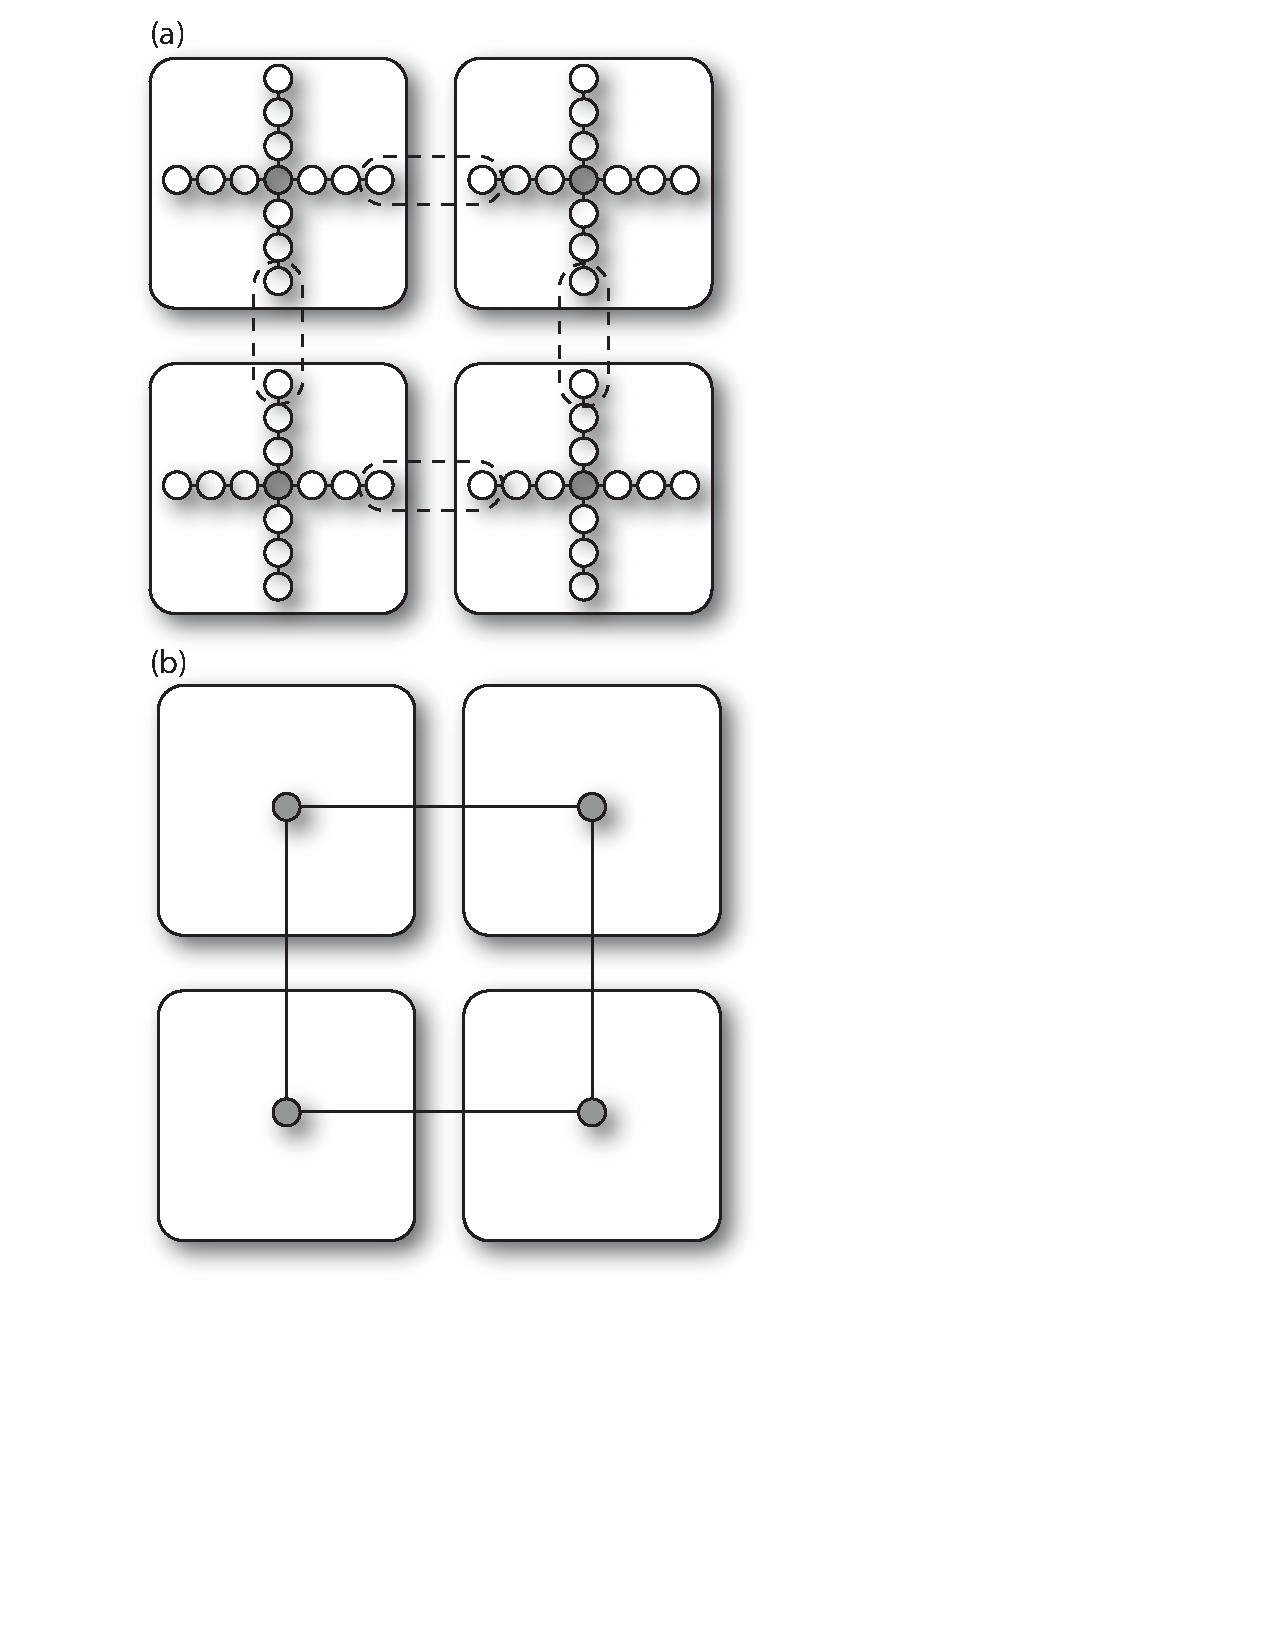
\includegraphics[width=0.4\textwidth]{module}
\caption{The modularised approach to scalable and economically efficient, distributed quantum computation using cluster states. The modules are all identical, and can be arbitrarily patched to one another, allowing the construction of arbitrary graph topologies. Because the modules are all identical, one might hope that mass production and economy of scale will drive down the cost of modules. We consider a simple \mbox{$2\times 2$} case where each module (rounded rectangles) comprises a single logical qubit (centre of each module in grey) and a number of ancillary qubits (white in each module), which facilitate bonding the logical qubits of nearest neighbours. The preparation of the modules is performed via nearest neighbour EOs (dashed ellipses), beginning at the end of branches, and working towards the root node upon each failure, until (hopefully) an EO is successful. (a) A \mbox{$2\times 2$} lattice of modules with their respective ancillary qubits. We attempt to bond the endpoints of chains using EOs. (b) Upon measuring the remaining ancillary qubits in the $\hat{Y}$ basis, only the logical qubits remain, with nearest neighbour bonds between adjacent modules, creating a distributed cluster state.} \label{fig:module}
\end{figure}

This approach has been shown to be resource-efficient \cite{bib:YoranReznik03, bib:Nielsen04}. Let us perform a rudimentary analysis of the resource scaling of this type of approach. The probability of successfully creating an edge between two modules is,
\begin{align}
p_\text{success} = 1 - {p_\text{failure}}^{n_\text{ancilla}},
\end{align}
where $p_\text{success}$ is the probability of joining two modules, $p_\text{failure}$ is the probability that a single EO fails, and $n_\text{ancilla}$ is the number of ancillary qubits per chain. $p_\text{success}$ can be made arbitrarily close to unity with sufficiently long ancillary chains, the required length of whom scales as,
\begin{align}
n_\text{ancilla} = \frac{\text{log}(1-p_\text{success})}{\text{log}(p_\text{failure})}.
\end{align}

Now, for simplicity we will consider the preparation of linear cluster states, although these ideas can easily be extended to more complex topologies, such as 2D lattice graphs.

Let us assume we have a `primary' linear topology of modules, which we will incrementally attempt to `grow' by tacking on new modules to the end. When we do so, with probability $p_\text{success}$ we grow the length of the primary by 1, otherwise we decrement it by 1. This proceeds as a random walk, with on average \mbox{$2p_\text{success}-1$} new qubits added to the primary per time-step. Provided this number is positive, i.e \mbox{$p_\text{success}>1/2$}, which can always be achieved with sufficient $n_\text{ancilla}$, the length of the primary grows linearly over time, allowing efficient state preparation.

This is just a very primitive model for preparing linear cluster states, using an equally primitive \textsc{Incremental} strategy for constructing them using non-deterministic gates. As discussed in Sec.~\ref{sec:CSQC}, much further work has been performed on the resource scaling of efficiently preparing cluster states of different graph topologies using different non-deterministic bonding strategies.

Of course, we have used the most simple model for modules, where each accommodates a single logical qubit. In due course, we would expect commodity modules to become far more capable, and resource scaling to improve. We might envisage that each module houses a small square lattice of logical qubits, as shown in Fig.~\ref{fig:larger_module}, and the interconnects between them glue them together like a patchwork quilt.

\begin{figure}[!htb]
\includegraphics[width=0.3\textwidth]{larger_module}
\caption{A larger cluster state module comprising a \mbox{$3\times 3$} lattice of logical qubits (grey), and dangling arms of ancillary qubits (white) in each direction for joining them to neighbouring modules. Fusing these modules enables the `patchwork' preparation of large, distributed lattices.} \label{fig:larger_module}
\end{figure}

%
% Fundamental Physics Experiments
%

\subsection{Outsourced quantum research} \index{Outsourced quantum research}\index{Fundamental physics experiments}

Thus far we have focussed on computation as the key utility for outsourced quantum technologies, and certainly this is likely to be the dominant driving force behind quantum outsourcing\index{Outsourced quantum technology}. But of course not everyone wants to only solve complex algorithmic problems. Others may wish to study quantum systems themselves from the perspective of basic science research\index{Basic science research}.

It is foreseeable that in the context of a true quantum internet, there will be a demand for not only the communication of bits and qubits, but more general `quantum assets'\index{Quantum assets} (Secs.~\ref{sec:introduction} \& \ref{sec:quant_net}), involving all manner of state preparation, manipulation, evolution and measurement, potentially all performed by different interconnected parties, specialising in different aspects of quantum protocols. The demand for this will extend far beyond computation.

The availability of a globe-spanning quantum network on satellites brings the opportunity for fundamental quantum mechanical experiments and unprecedented length scales and velocities in the future. Satellite-to-satellite\index{Satellite-to-satellite} photon transfer can allow for ultra-long distance quantum communications that are not possible on Earth due to atmospheric loss. Another unique aspect of space is that satellites move at high velocities -- typically at $10^{-5} $ times the speed of light\index{Speed of light} for LEO satellites. The combination of both of these effects gives a unique opportunity for performing relativistic quantum information\index{Relativistic quantum information} experiments to test fundamental physics. 

We anticipate that some of the first experiments will be extensions of what are already performed on Earth. For example, one can perform increasingly long space-based Bell violation tests\index{Bell violation} at unprecedented distances \cite{bib:yin2017satellite}. Another possibility is to examine the speed of influence of entanglement, which bound the speed of entanglement \cite{bib:yin2013lower}. In space, such experiments could be extended much further, giving tighter bounds. There are demanding technical hurdles that must be overcome to succeed at such experiments, such as the necessity for synchronised clocks (Sec.~\ref{sec:clocks}).

 In addition to examining extensions of existing experiments, the high satellite velocities can be used to perform relativistic quantum information experiments, such as entanglement tests in the presence of special\index{Special relativity} and general relativity\index{General relativity}, Wheeler's delayed choice experiment\index{Wheeler's delayed choice experiment}, and enhanced quantum metrology \cite{sec:kaltenbaek2003proof, sec:scheidl2013quantum, sec:ahmadi2014relativistic}.

The QTCP protocol presented in Sec.~\ref{sec:QTCP} provides an extensible framework for facilitating these kinds of outsourced or delegated protocols\index{Outsourced protocols}\index{Delegated protocols} using generic quantum assets. Bear in mind that, as designed, the payload of QTCP packets could encapsulate all manner of optical states, or mediate long-distance interaction between them.

This model for quantum research could be invaluable to less-well-resourced researchers, for example in developing nations or not-so-well-funded universities, opening up a field of experimental research previously inaccessible to them. Indeed, some private and university sector operators are making elementary, remotely programmable quantum information processing protocols available over the internet, bringing this type of research within reach of researchers and even curious hobbyists around the globe.

While such early implementations fall far short of being truly reconfigurable, outsourced or delegated quantum protocols, applicable to a broad range of applications, they certainly already demonstrate the interest such models for outsourcing is generating within the research community, and the viability of further extending it.

Examples of how this type of model might be applied could include, but not be limited to research into:
\begin{itemize}
	\item Quantum information processing protocols, beyond only quantum computation, bits and qubits.
	\item Bose-Einstein condensates (BECs)\index{Bose-Einstein condensates (BECs)}.
	\item Light-matter interactions.\index{Light-matter interactions}
	\item Quantum thermodynamics and quantum statistical mechanics.\index{Quantum thermodynamics}\index{Quantum statistical mechanics}
	\item Quantum phase-transitions.\index{Quantum phase-transitions}
	\item Quantum optics, involving all manner of quantum states of light, beyond only those raised in Sec.~\ref{sec:opt_enc_of_qi}.\index{Quantum optics}
	\item Optical interferometry.\index{Optical interferometry}
\end{itemize}

In some instances, such outsourced quantum protocols might be applicable to encryption protocols, like those discussed in the next section, Sec.~\ref{sec:homo_blind}, enabling highly valuable secrecy for the experiments being conducted by researchers and their hard-earned results\footnote{Note, however, that the upcoming protocols are designed for application to particular optical states and protocols, and encryption schemes involving more generic quantum assets are likely to require some rethinking and adaptation (if possible at all, which isn't guaranteed!).}.

\latinquote{Timendi causa est nescire.}

%%
% Encrypted Cloud Quantum Computation
%

\section{Encrypted cloud quantum computation} \label{sec:homo_blind} \index{Encrypted quantum computation}

\sectionby{Atul Mantri, Si-Hui Tan \& Peter Rohde}\index{Atul Mantri}

\dropcap{E}{xtremely} important to many high-performance data-processing applications is security, as proprietary or sensitive data may be being dealt with. To address this, there are two models for encrypted, outsourced quantum computation -- \textit{homomorphic encryption} \cite{bib:gentry2009fully, bib:van2010fully}\index{Homomorphic encryption} and \textit{blind quantum computation}\index{Blind quantum computation} \cite{bib:blind2, bib:broadbent2009universal, bib:barz2012demonstration, bib:PhysRevLett.108.200502, bib:Morimae3486, bib:Morimae5460, bib:Morimae5460}.

In both cases, Alice has secret data$^\copyright$, and wishes to not only ensure that an interceptor is unable to read it, but that even the server performing the computation isn't able to either -- she trusts no one. That is, she wishes the data to be processed in encrypted form, without first requiring decryption.

The difference between the two protocols lies in the treatment of algorithms:
\begin{itemize}
	\item Homomorphic encryption: Alice provides only the data, whereas Bob provides the processing and the algorithm it implements (which he would also like to keep to himself in general). When \textit{any} circuit is allowed, the protocol is said to be a \textit{fully homomorphic} encryption protocol (FHE). Otherwise, it is a \textit{somewhat-homomorphic} encryption protocol. Although homomorphic encryption protocols have been around for a few decades in the form of privacy homomorphisms \cite{bib:Rivest1978}, classical FHE has only been described very recently \cite{bib:gentry2009fully, bib:van2010fully}.
	\item Blind quantum computing: Alice provides both the algorithm \textit{and} the data, and wishes \textit{both} to remain secret to her. It is known that universal blind \textit{classical} computation is not possible, universal blind \textit{quantum} computation is.
\end{itemize}
Both of these seem like very challenging goals, yet significant developments have been made on both fronts in the quantum world, with efficient resource overheads associated with the encryption.

In the usual circuit model, blind quantum computation has been shown to be viable, and optimal bounds derived. Equivalently, such protocols have been described in the cluster state model (Sec.~\ref{sec:CSQC}). For universal computation, such protocols necessarily require classical interaction between the client and host. However, it was shown that in some restricted (i.e non-universal) models for optical quantum computation, specifically \textsc{BosonSampling}, quantum walks and coherent state passive linear optics, non-interactive, somewhat-homomorphic encryption may be implemented.

These encryption protocols induce a resource overhead in circuit size and number of qubits involved in the computation, with efficient scaling. They deliver (at least partially) information-theoretically secure (Sec.~\ref{sec:comp_vs_inf_th_sec}) data-hiding, enabling trustworthy outsourced processing of encrypted data, independent of the attack.

%
% Classical Computation 
%

\subsection{Classical computation} \index{Classical encrypted computation}
\comment{A universal QC can implement any classical algorithm. So QCs with homo/BQC give us the means by which to perform encrypted classical computations, bypassing limitations imposed by purely classical protocols.}
\comment{[Comment: The polynomial hierarchy is not contained in BQP. In fact, NP-complete problems are not contained in BQP.]}


To set the stage for our upcoming treatment of encrypted quantum computation protocols, we begin by reviewing recent developments in \textit{classical} homomorphic encryption, paying special interest to resource scaling and information-theoretic security.

\comment{The first FHE scheme was reported in Gentry's seminal paper \cite{bib:gentry2009fully}. He showed that if a homomorphic encryption scheme can evaluate its own decryption circuit, and also slightly augmented versions of it--a feature he calls {\it bootstrapping}, one can construct a FHE scheme from it. Then he constructed a somewhat homomorphic encryption protocol using ideal lattices, and via a clever transformation that decreases the complexity of its decryption circuit, showed that it is bootstrappable with respect to a universal set of gates. For a security parameter $\lambda$, Gentry's scheme has a $\widetilde{O}(\lambda^6)$ \footnote{The tilde in the big-O notation means that we are ignoring logarithmic factors.} bit bound on complexity for refreshing a ciphertext corresponding to a 1-bit plaintext \cite{bib:Gentrythesis}. This was subsequently reduced to $\widetilde{O}(\lambda^{3.5})$ \cite{bib:Damien2010}, $\widetilde{O}(\lambda)$ \cite{bib:Brakerski2011}, and ${\rm polylog (\lambda)}$ for any width-$\Omega(\lambda)$ circuit with $t$ gates \cite{bib:Craig2012}. }

\comment{A homomorphic encryption scheme is made up of four algorithms: a key generation algorithm, \textsc{KeyGen}, an encryption algorithm, \textsc{Encrypt}, an evaluation algorithm, \textsc{Evaluate}, and a decryption algorithm, \textsc{Decrypt}. The four algorithms have the following inputs and outputs:
\begin{itemize}
\item \textsc{KeyGen}$(\lambda)$: Takes as input a security parameter $\lambda$, and outputs a public-key $pk$, and a secret-key $sk$.
\item \textsc{Encrypt}$(pk, \pi_i)$: Takes as input $pk$, and a plaintext $\pi_i$. It outputs a ciphertext $\psi_i$.
\item \textsc{Evaluate}$(pk, C, \Psi)$: Takes as input $pk$, a permitted circuit $C$, and $\Psi=(\psi_1,\ldots, \psi_t)$. It outputs a ciphertext $\psi$.
\item \textsc{Decrypt}$(sk,\psi)$: Takes as input $sk$, and $\psi$ and outputs $C(\pi_1,\ldots, \pi_t)$.
\end{itemize}
The computational complexity of all these algorithms must be polynomial in $\lambda$, and in the case of the evaluation algorithm, polynomial in the size of the evaluation circuit $C$. The condition that \textsc{Decrypt}$(sk,\psi)$ outputs $C(\pi_1,\ldots, \pi_t)$ is a condition known as correctness which we require of the homomorphic encryption scheme. Furthermore, we also require ciphertext size and decryption time to be upper bounded by a function of the security parameter $\lambda$, independently of $C$. This last condition is known as compactness, and is necessary to exclude trivial schemes such as that which decrypts the ciphertexts first, and then apply $C$.}

\comment{The specifics of these algorithm vary from scheme to scheme, and as is in the case of FHE, usually contains sub-algorithms within them. Making FHE practical is an active area of research. Much of the problem lies in the bootstrapping required in Gentry's scheme, and some of these efforts lies in reducing the overhead required in bootstrapping or removing the need for bootstrapping entirely. Although there exists a plethora of FHE schemes, they are based mainly on two types of problems in lattice-based cryptography: the Shortest Vector Problem (SVP), and Learning with Errors (LWE) Problem. Gentry's original FHE was based on SVP, but over time, the schemes have moved towards a LWE approach because they offer lower overhead and are conceptually simpler . An overview of advances, and applications of homomorphic encryption can be found in a recent review \cite{bib:Halevi2017}.}

%
% Homomorphic Encryption
%

\subsubsection{Homomorphic encryption} \index{Homomorphic encryption}

\comment{To do!}
Yes
%
% Blind Computation
%

\subsubsection{Blind computation} \index{Blind quantum computation}

\comment{To do!}

%
% Cluster States
%

\subsection{Cluster states} \index{Encrypted quantum computation!Cluster states}

Most simply, if Alice has the limited quantum resources required to perform single-qubit measurements, and she knows the algorithm she wishes to implement, then by outsourcing just the cluster state preparation stage, whilst performing the single-qubit measurements herself, she can obviously obtain \textit{perfect} secrecy of both her data and her algorithm, since no one else is involved in the processing stage.

However, Alice may have access to no quantum resources whatsoever -- even single-qubit measurements -- requiring homomorphic encryption or blind quantum computing protocols that are native to the cluster state model. Both such protocols have been described, and in fact are conceptually more straightforward to understand in the cluster state formalism. 

\comment{To do}

\comment{Consider both BQC and homomorphic QC}

%
% Homomorphic Encryption
%

\subsubsection{Homomorphic encryption} \index{Homomorphic encryption}

\comment{To do!}

%
% Blind Quantum Computation
%

\subsubsection{Blind quantum computation} \index{Blind quantum computation}

\comment{To do!}

%
% Circuit Model
%

\subsection{Circuit model} \index{Encrypted quantum computation!Circuit model}

\comment{To do}

%
% Homomorphic Encryption
%

\subsubsection{Homomorphic encryption} \index{Homomorphic encryption}

\comment{To do!}

%
% Blind Quantum Computation
%

\subsubsection{Blind quantum computation} \index{Blind quantum computation}

\comment{To do!}

%
% Encryption Passive Optics
%

\subsection{Passive optics} \index{Encrypted quantum computation!Passive optics}

The previously discussed schemes for encrypted universal quantum computation required a degree of client/server interaction via classical communication. But perhaps there are some restricted (i.e non-universal) models for optical quantum computation, which lend themselves to passive, non-interactive encryption? And perhaps these restrictions simplify the physical resource requirements for encryption?

Let us formalise some reasonable requirements for such a scheme. We will require that:
\begin{itemize}
\item Alice's encoding (state preparation) and decoding (measurement) operations are separable, single-mode operations (i.e she has no quantum power of entanglement at her disposal).
\item Bob's computation is non-interactive, requiring no input from Alice beyond her input state.
\item Bob's computation is passive, requiring no intermediate measurement and feedforward.
\item Other than this, there are no constraints on the structure of the encoding/decoding operations, or the optical quantum computation being implemented (e.g it could encompass more than just linear optics).
\end{itemize}

We can express these requirements very generally and elegantly in terms of a commutation relation between the encoding ($\hat{E}$), decoding ($\hat{D}$), and computational ($\hat{U}$) operations. Furthermore, for the protocol to hide information, the plaintext basis states must not be invariant under the encoding operations. This enforces the criteria,
\index{Criteria for encrypted passive optics}
\begin{definition}[Encrypted passive optics] \label{def:enc_pass}
Let \mbox{$k=\{k_1,\dots,k_m\}$} be a partition of the key $k$ into sub-keys $\{k_i\}$, one associated with each mode $i$. Let $\hat{E}_i(k_i)$ and $\hat{D}_i(\tilde k_i)$ be the encoding and decoding operations for the $i$th mode. $\tilde k$ is a potentially transformed version of $k$, to accommodate that the encryption and decryption keys may be asymmetric, in which case we require that $\tilde{k}$ be efficiently computable from $k$. Let $\hat{U}$ be the computation. Then, separability of the encoding and decoding operations requires the following commutation relation to hold,
\begin{align} \label{eq:gen_pass_hom}
\hat{U} \left[\bigotimes_{i=1}^m\hat{E}_i(k_i)\right] = \left[\bigotimes_{i=1}^m\hat{D}^\dag_i(\tilde k_i)\right] \hat{U}.
\end{align}
For the protocol to hide information, the plaintext basis states must not be invariant under the encoding operations,
\begin{align}
\left[\bigotimes_{i=1}^m\hat{E}_i(k_i)\right]\ket\psi_\mathrm{plaintext} \neq \ket\psi_\mathrm{plaintext}.
\end{align}
The state observed by Bob is the mixture of Alice's plaintext over the complete set of encoding operations, implementing a quantum process $\mathcal{E}$, with Kraus operators $\hat{E}(k)$,
\begin{align} \label{eq:mix_over_enc_ops}
\hat\rho_\mathrm{encoded} &= \mathcal{E}(\ket\psi_\mathrm{plaintext}\bra\psi_\mathrm{plaintext}) \nonumber \\
&= \sum_k \hat{E}(k)\ket\psi_\mathrm{plaintext}\bra\psi_\mathrm{plaintext} \hat{E}^\dag(k),
\end{align}
where,
\begin{align}
\hat{E}(k) = \bigotimes_{i=1}^m\hat{E}_i(k_i).
\end{align}
To minimise Bob's chances of guessing Alice's state, we would like to maximise the von Neuman entropy of Bob's state. For \mbox{$S(\hat\rho_\mathrm{encoded})=0$} we have no secrecy, whereas for maximal \mbox{$S(\hat\rho_\mathrm{encoded})$} we have maximal secrecy (for the given plaintext basis state).
\end{definition} 

Intuitively, this simply says that a tensor product of single-mode encoding operations commutes through the passive computation to yield a (potentially different) tensor product of single-mode decoding operations. This way, Alice's operations are all separable, requiring no entangling gates (after all, if she had access to entangling gates she might be able to do quantum computations herself!). This relationship can be illustrated as shown in Fig.~\ref{fig:gen_pass_hom}.

Importantly, note that devising a scheme satisfying this commutation relation does not automatically imply that it is secure -- it merely enforces the separability of Alice's encoding and decoding operations. An actual security proof is far more demanding, and will be highly state-dependent.

\begin{figure}[!htbp]
\includegraphics[clip=true, width=0.425\textwidth]{gen_pass_hom}
\captionspacefig \caption{General structure for the relationship between the encoding ($\hat{E}$), decoding ($\hat{D}$), and computational ($\hat{U}$) operations in a passive, non-interactive, optical quantum computation, where Alice is restricted to non-entangling, single-mode encoding and decoding operations.} \label{fig:gen_pass_hom}
\end{figure}

In the following sections we introduce non-interactive techniques for passive optical quantum computation based upon this general formalism. As encoding techniques compatible with the commutation relation from Eq.~(\ref{eq:gen_pass_hom}), we specifically introduce:
\begin{itemize}
\item \textit{Polarisation-key encoding} (Sec.~\ref{sec:phot_homo_enc}): a uniform random polarisation rotation is applied to each input mode, which we apply to photonic linear optics.\index{Polarisation!Key encoding}
\item \textit{Phase-key encoding} (Sec.~\ref{sec:homo_coherent_state}): a uniform random phase-shift is applied to each input mode, which we apply to the encryption of coherent states under evolution via linear optics and generalised non-linear phase-shift operations.\index{Phase!Key encoding}
\item \textit{Displacement-key encoding} (Sec.~\ref{sec:disp_key_enc}): an arbitrary configuration of random phase-space displacements is applied to the input modes, which in principle applies to any optical encoding.\index{Displacement-key encoding}
\end{itemize}
However, we leave it as an open question for future work to fully characterise the set of compatible encoding, decoding and computational operations, and to evaluate their security for different choices of input states.

%
% Polarisation-Key Encoding
%

\subsubsection{Polarisation-key encoding} \label{sec:phot_homo_enc} \index{Polarisation!Key encoding}

It was recently shown that processing photonic states using passive linear optics -- i.e \textsc{BosonSampling} or quantum walks (Secs.~\ref{sec:boson_sampling} \& \ref{sec:QW}) -- may be trivially homomorphically encrypted with the addition of additional photons and randomised polarisation rotations on the inputs \cite{bib:RohdeQWEnc12}, so-called \textit{polarisation-key encoding}. This encryption does not require any client/server interaction, remaining completely passive, yet achieving near optimal secrecy, hiding $O(\log (m))$ bits of information in an $m$-mode interferometer. Furthermore, it does not impose an overhead in circuit complexity, only in the number of input photons.

For $m$ modes, the resource requirements are:
\begin{enumerate}
\item $m$ single-photons -- one per input mode.
\item $m$ classically controlled wave-plates, able to implement arbitrary polarisation rotations.
\item $m$ polarisation filters.
\item $m$ photo-detectors.
\item An \mbox{$m\times m$} linear optics network.
\end{enumerate}
The full protocol is described in Alg.~\ref{alg:homo_LO} and shown in Fig.~\ref{fig:BS_homo}.

\begin{table}[!htbp]
\begin{mdframed}[innertopmargin=3pt, innerbottommargin=3pt, nobreak]
\texttt{
function PolarisationKeyEncoding($S$,$k$):
\begin{enumerate}
    \item Alice meditates upon, but needn't actually prepare the state,
    \begin{align}
    \ket\psi_\mathrm{number} = \ket{S_1,\dots,S_m},    
    \end{align}
    where,
    \begin{align}
S_i\in\{0,1\},
    \end{align}
is the photon-number of the $i$th mode.
   \item Alice makes the substitutions from the photon-number basis into the polarisation basis, 
   \begin{align}
   \ket{0}&\to\ket{H}, \nonumber \\
   \ket{1}&\to\ket{V},
   \end{align}
   to obtain $\ket\psi_\mathrm{pol}$, containing $m$ photons in total, one per mode.
   \item Alice chooses a random private-key $k$ as a real number from the uniform distribution,
   \begin{align}
    k\in(0,2\pi).
    \end{align}
    \item Alice prepares the encoded state by applying the same polarisation rotation (using wave-plates), of angle $k$, to each mode,
   \begin{align}
   \ket\psi_\mathrm{enc} = \hat{R}(k)^{\otimes m}\ket\psi_\mathrm{pol},
   \end{align}
   where,
   \begin{align}
   \hat{R}(\theta) = \begin{pmatrix}
\cos\theta & -\sin\theta \\
\sin\theta & \cos\theta
\end{pmatrix}.
   \end{align}
    \item Alice sends $\ket\psi_\mathrm{enc}$ to Bob.
    \item Bob applies processing using his linear optics computer, to obtain,
    \begin{align}
    \ket\psi_\mathrm{enc\,comp} = \hat{U} \ket\psi_\mathrm{enc}.
    \end{align}
    \item Bob returns $\ket\psi_\mathrm{enc\,comp}$ to Alice.
    \item Alice applies the inverse of the encoding operation,
    \begin{align}
    \ket\psi_\mathrm{comp} = \hat{R}(-k)^{\otimes m}\ket\psi_\mathrm{enc\,comp}.
    \end{align}
    \item Alice applies polarisation filters to $\ket\psi_\mathrm{comp}$, discarding horizontally polarised photons.
    \item The remaining vertically polarised state is Alice's unencrypted output of the computation.
    \item $\Box$
\end{enumerate}}
\end{mdframed}
\captionspacealg \caption{Protocol for implementing homomorphic encryption on photonic passive linear optics, using polarisation-key encoding.} \label{alg:homo_LO}
\end{table}

\begin{figure}[!htbp]
\includegraphics[clip=true, width=0.425\textwidth]{BS_homo}
\captionspacefig \caption{Protocol for implementing homomorphic encryption on photonic passive linear optics. Horizontal bars are wave-plates, implementing polarisation rotations $\hat{R}(\theta)$ -- the encryption and decryption operations performed by Alice. $\ket\psi_\mathrm{in}$ contains one photon per mode, polarisation-encoded such that vertically polarised photons belong to the desired computation, whilst the remaining horizontally polarised ones are dummies. The polarisation rotation angle, $k$, acts as Alice's private-key. The photo-detectors are polarisation-resolving, discarding all dummy horizontally polarised photons at the output. The algorithm is described in detail in Alg.~\ref{alg:homo_LO}.} \label{fig:BS_homo}
\end{figure}

The key idea here is that orthogonal polarisations do not interfere with one another under linear optics evolution. Thus, by inserting additional orthogonally polarised `dummy' photons, and applying uniform, random polarisation rotations, we can confuse any eavesdropper as to which photons belong to the computation, thereby hiding the secret data from them. Note that the encryption protocol does not affect the computation, since uniform polarisation rotations commute through linear optics circuits,
\begin{align} \label{eq:LO_key_commute}
\hat{R}(k)^{\otimes m} \hat{U} \hat{R}(-k)^{\otimes m} = \hat{R}(k)^{\otimes m} \hat{R}(-k)^{\otimes m} \hat{U} = \hat{U},
\end{align}
using the identity,
\begin{align}
\hat{R}(-k) = \hat{R}^\dag(k).	
\end{align}

Practically, $k$ could be chosen as some integer multiple of \mbox{$2\pi/d$}, where $d$ is the number of distinct keys, since an infinite precision key would be equivalent to an infinitely long key, were it represented as a bit-string. In this case, the information security of the protocol increases with $d$.

\cite{bib:RohdeQWEnc12} provided two relationships for the security of this protocol. First, the probability of Bob guessing Alice's input string approaches,
\begin{align}
P_\mathrm{guess} \leq \sqrt{\frac{8}{\pi m}},
\end{align}
for sufficiently large $m$ and $d$, which asymptotically (but unfortunately only polynomially\footnote{Note that an exponentially small bound is actually prohibited by no-go theorems for oblivious transfer and bit commitment \cite{bib:HKLo97, bib:SpekkensRudolphSecure}}) approaches 0.

Alternately, the mutual information between Alice and Bob, \mbox{$I(A;B)$}, can be upper-bounded using the Holevo quantity, $\chi$ \cite{bib:HolevoQuantity}. That is, \mbox{$I(A;B)\leq\chi$}. The Holevo quantity is defined as,\index{Holevo quantity}
\begin{align}
\chi = S(\hat\rho) - \sum_i p_i S(\hat\rho_i),
\end{align}
where,
\begin{align}
\hat\rho = \sum_i p_i \hat\rho_i,
\end{align}
and $S(\cdot)$ denotes the von Neuman entropy\index{von Neuman entropy} (Sec.~\ref{sec:channel_cap}). Here $\hat\rho_i$ are the individual codewords, in our case the set of all polarisation-encoded basis states, and $p_i$ are their respective probabilities, which are uniform here.

The upper-bound stipulated by the Holevo quantity is an information-theoretic bound\index{Information-theoretic!Bound}, which holds under \textit{any} choice of measurement bases by Bob. Thus, it is impossible for Bob to extract more information about Alice's state than allowed by this bound.

For this protocol the Holevo quantity scales with the number of modes as,
\begin{align}
\chi(m) = m - \frac{1}{2}\log_2\left(\frac{\pi e m}{2}\right) + O\left(\frac{1}{m}\right),
\end{align}
for sufficiently large $d$. Since there are $m$ bits of information in Alice's input state, this implies that the protocol hides at least,
\begin{align}
\frac{1}{2}\log_2\left(\frac{\pi e m}{2}\right) + O\left(\frac{1}{m}\right),
\end{align}
bits of information from Bob.

Furthermore, because a single computation requires Alice to perform only a single call to Bob's algorithm, which we treat as a black box, Alice gains minimum knowledge about Bob's secret algorithm, which is optimal for Bob.

Note that while we have considered linear optics in the above discussion, we could in fact expand the list of ingredients available to the computation to include anything generated by a Hamiltonian that commutes with polarisation rotations,
\begin{align}
[\hat{R}(\theta),\hat{H}]=0.
\end{align}
This could include, for example, polarisation-independent non-linear operations.

\comment{Discuss follow-up paper by Fitzsimons group on using other photonic degrees of freedom to enhance security.}

%
% Phase-Key Encoding
%

\subsubsection{Phase-key encoding} \label{sec:homo_coherent_state} \index{Phase!Key encoding}

As discussed in Sec.~\ref{sec:coherent_state_QC}, although not a \textit{quantum} computation, a system comprising multi-mode coherent state inputs, evolved via passive linear optics, implements simple matrix multiplication on the vector of input coherent state amplitudes,
\begin{align} \label{eq:betaUalpha}
\vec\beta = U\cdot\vec\alpha,
\end{align}
for input,
\begin{align}
\ket{\vec\alpha}=\ket{\alpha_1,\dots,\alpha_m},
\end{align}
and output,
\begin{align}
\ket{\vec\beta}=\ket{\beta_1,\dots,\beta_m}.
\end{align}
However, despite this being a classically efficient algorithm, it can experimentally be easily homomorphically encrypted with no computational resource overhead. This is in contrast to classical homomorphic encryption techniques, which incur a computational overhead.

The idea behind homomorphic encryption of coherent state linear optics is conceptually almost identical to the polarisation-space protocol for photonic linear optics (Sec.~\ref{sec:phot_homo_enc}). The key difference is that the random rotations are no longer applied in polarisation-space, but in phase-space as phase-rotations (\textit{phase-key encoding}). Specifically, the encryption/decryption operations are now given by the phase-shift operators, 
\begin{align}
\hat{R}(\phi) = \hat\Phi(\phi)=e^{-i\phi\hat{n}}.
\end{align}
Phase-shift operators acting on coherent states simply implement the transformation,
\begin{align}
\hat\Phi(\phi)\ket\alpha = \ket{e^{-i\phi}\alpha},
\end{align}
a simple rotation about the origin in phase-space.

Like polarisation rotations, uniform phase-shifts commute through linear optics networks, as per Eq.~(\ref{eq:LO_key_commute}), and thus the protocol has similar mathematical structure to the photonic case. Now the phase-shift angle, $\phi$, acts as Alice's private-key, which she applies uniformly to all input modes, applying inverse uniform phase-shifts after the computation to decrypt the state. The full algorithm is given in Alg.~\ref{alg:homo_coherent_LO}.

\begin{table}[!htbp]
\begin{mdframed}[innertopmargin=3pt, innerbottommargin=3pt, nobreak]
\texttt{
function PhaseKeyEncoding($\vec\alpha$,$k$):
\begin{enumerate}
    \item Alice prepares the input multi-mode coherent state,
    \begin{align}
    \ket\psi_\mathrm{in} = \ket{\vec\alpha} = \ket{\alpha_1,\dots,\alpha_m}.
    \end{align}
    \item Alice chooses a random private-key $k$ as a real number from the uniform distribution,
    \begin{align}
    k\in (0,2\pi).
    \end{align}
    \item Alice prepares the encoded state by applying the same phase-shift, of angle $k$, to each mode,
    \begin{align}
    \ket\psi_\mathrm{enc} = \hat\Phi(k)^{\otimes m}\ket\psi_\mathrm{in},
    \end{align}
    where,
    \begin{align}
    \hat\Phi(\phi) = e^{i\phi\hat{n}},
    \end{align}
    is the phase-shift operator.
    \item Alice sends $\ket\psi_\mathrm{enc}$ to Bob.
    \item Bob applies processing using his linear optics computer, to obtain,
    \begin{align}
    \ket\psi_\mathrm{enc\,comp} = \hat{U}\ket\psi_\mathrm{enc}.
    \end{align}
    \item Bob returns $\ket\psi_\mathrm{enc\,comp}$ to Alice.
    \item Alice applies the inverse of the encoding operation,
    \begin{align}
    \ket\psi_\mathrm{comp} = \hat\Phi(-k)^{\otimes m}\ket\psi_\mathrm{enc\,comp}.
    \end{align}
    \item The resulting state is,
    \begin{align}
    \ket\psi_\mathrm{comp} = \ket{\vec\beta} = \ket{\beta_1,\dots,\beta_m},
    \end{align}
    where,
    \begin{align}
    \vec\beta = U\cdot\vec\alpha.
    \end{align}
    \item $\Box$
\end{enumerate}}
\end{mdframed}
\captionspacealg \caption{Protocol for implementing homomorphic encryption on coherent state passive linear optics, using phase-key encoding.} \label{alg:homo_coherent_LO}
\end{table}

In fact, this encryption technique applies to more than just linear optics, but extends to also include generalised non-linear phase-shift operations, generated by Hamiltonians that are polynomials in the photon-number operators,
\begin{align}
\hat{H} = O(\mathrm{poly}(\hat{n}_1,\dots,\hat{n}_m)),
\end{align}
where $\hat{n}_i$ is the photon-number operator for the $i$th mode\index{Photon-number!Operators}. This observation follows trivially from the observation that the phase-shift encoding operations (which are generated by Hamiltonians linear in the photon-number operators) commute with any polynomial in the photon-number operators,
\begin{align}
[\hat{n}_i,\mathrm{poly}(\hat{n}_1,\dots,\hat{n}_m)] = 0\,\,\forall \, i.
\end{align}
This immediately significantly expands the class of operations available for the computation. In particular, while coherent states remain separable under linear optics evolution, the introduction of non-linear phase-shift operations enables quantum entanglement, and presumably a more powerful class of computations than simple matrix multiplication. It is unclear to us, however, exactly what this class of computations actually is.

\cite{siHuiTan} evaluated the security of this protocol in the case where the basis states were restricted to the binary $\ket{\pm\alpha}$ states. Thus, each input mode encodes at most a single bit (zero bits for \mbox{$|\alpha|=0$}, approaching one bit for \mbox{$|\alpha|\to\infty$}). Rather than employing the mutual information, they resorted to the alternative approach of calculating the distinguishability of codewords under the trace distance (Sec.~\ref{sec:fid_metric}). This has a direct operational interpretation as the probability of Bob guessing Alice's state in the best case. If the basis codeword states observed by Bob are indistinguishable, they are effectively decorrelated from the plaintext basis states, preventing him from guessing Alice's plaintext state, whereas if they are distinguishable, he can.

Let $\vec{x}$ be the binary input string, and $\vec{0}$ be the special case of the all-zero string. Then, for unencrypted states, we have the trace distance,
\begin{align}
D_\mathrm{unenc} &= ||\hat\rho_{\vec{x}}-\hat\rho_{\vec{0}}||_\mathrm{tr} \nonumber \\
&= \sqrt{1-e^{-4\mathrm{wt}(\vec{x})|\alpha|^2}},
\end{align}
where $\mathrm{wt}(\vec{x})$ is the Hamming weight (number of 1s in the bit-string) of $\vec{x}$. On the other hand, for the encoded states, we have,
\begin{align}
D_\mathrm{enc} &= ||\mathcal{E}(\hat\rho_{\vec{x}})-\mathcal{E}(\hat\rho_{\vec{0}})||_\mathrm{tr} \\
&= \sum_{k=0}^{d-1} e^{-m|\alpha|^2}\frac{(m|\alpha|^2)^k}{k!}\sqrt{1-\left(\frac{m-2\mathrm{wt}(\vec{x})}{m}\right)^{2k}}, \nonumber
\end{align}
\comment{What's the limit as $d\to\infty$?} where $\mathcal{E}$ denotes the mixture over encoding operations observed by Bob, as per Eq.~(\ref{eq:mix_over_enc_ops}), and there are $d$ distinct keys. We also define the ratio between these two distances,
\begin{align}
R=\frac{D_\mathrm{enc}}{D_\mathrm{unenc}	},
\end{align}
as an indicator of data-hiding. \mbox{$R<1$} is indicative that information is hidden from Bob.

These relationships are illustrated in Figs.~\ref{fig:homo_coh_st_tr} \& \ref{fig:homo_coh_st_ratio}\footnote{Note that the distance between any arbitrary pair of codewords may be obtained by replacing $\mathrm{wt}(\cdot)$ with their Hamming distance (in the simple case where one of the codewords is the $\vec{0}$ bit-string, the Hamming weight and Hamming distance are equivalent).}. Clearly, the encoded basis states exhibit greater indistinguishability than the unencoded ones, demonstrating that information is hidden from Bob. The trace distance does not have the elegant interpretation of `number of bits hidden' that the mutual information does. Rather, it gives us the probability of Bob correctly guessing Alice's state, demonstrating the degree of partial hiding of information.

\if 2\pubmode
\begin{figure}[!htbp]
\includegraphics[clip=true, width=0.475\textwidth]{coherent_state_homo_unenc}\\
\includegraphics[clip=true, width=0.475\textwidth]{coherent_state_homo_enc}
\captionspacefig \caption{Trace distance between unencoded (top) and encoded (bottom) basis states for coherent state computation using phase-key encoding, with \mbox{$d=50$} keys and \mbox{$m=10$} modes. Each mode is inputted with one of two basis coherent states, \mbox{$\ket{\pm\alpha}$}. \mbox{$\mathrm{wt}(\vec{x})$} denotes the Hamming weight of bit-string $\vec{x}$. Two states are indistinguishable if their trace distance is 0, and distinguishable (orthogonal) if their trace distance is 1. Lower trace distance between encoded states implies a lower chance of Bob guessing Alice's plaintext input state.} \label{fig:homo_coh_st_tr}
\end{figure}
\else
\begin{figure*}[!htbp]
\includegraphics[clip=true, width=0.475\textwidth]{coherent_state_homo_unenc}
\includegraphics[clip=true, width=0.475\textwidth]{coherent_state_homo_enc}
\captionspacefig \caption{Trace distance between unencoded (top) and encoded (bottom) basis states for coherent state computation using phase-key encoding, with \mbox{$d=50$} keys and \mbox{$m=10$} modes. Each mode is inputted with one of two basis coherent states, \mbox{$\ket{\pm\alpha}$}. \mbox{$\mathrm{wt}(\vec{x})$} denotes the Hamming weight of bit-string $\vec{x}$. Two states are indistinguishable if their trace distance is 0, and distinguishable (orthogonal) if their trace distance is 1. Lower trace distance between encoded states implies a lower chance of Bob guessing Alice's plaintext input state.} \label{fig:homo_coh_st_tr}
\end{figure*}
\fi

\begin{figure}[!htbp]
\includegraphics[clip=true, width=0.475\textwidth]{coherent_state_homo_ratio}
\captionspacefig \caption{Ratio of the trace distance between unencoded and encoded basis states for coherent state computation using phase-key encoding, with \mbox{$d=50$} keys and \mbox{$m=10$} modes. \mbox{$R<1$} implies information hiding from Bob.} \label{fig:homo_coh_st_ratio}
\end{figure}

It seems plausible that this approach to homomorphic encryption in phase-space could be extended to other quantum states of light. However, as is typically the case, performing entropic security proofs is notoriously difficult, and this remains an open problem. It should be noted, however, that this approach will definitely \textit{not} work for any class of input states which are invariant under phase-shifts. This explicitly rules out employing this technique for, for example, photon-number states, which have no phase.

This protocol demonstrates that a simple optical system is able to homomorphically encrypt the classical computation of matrix multiplication, as well as the more general operations of non-linear phase-shifts, without incurring the computational resource overhead imposed by conventional classical homomorphic encryption techniques.

\comment{Include figures for asymptotics against m and d.}

%
% Displacement-Key Encoding
%

\subsubsection{Displacement-key encoding} \label{sec:disp_key_enc} \index{Displacement-key encoding}

In the previous two sections we employed the encryption techniques of polarisation-key encoding and phase-key encoding. These are based on the observation that uniform polarisation- and phase-rotations commute through linear optics networks, as per Eq.~(\ref{eq:LO_key_commute}). Are there any other types of encoding operations that observe this property?

The other obvious candidate is \textit{displacement-key encoding}, whereby random displacements (not necessarily uniform across all modes) in phase-space (Sec.~\ref{sec:non_lin_opt}) form the encoding operations. Displacement operators exhibit the property that a tensor product of displacements commutes through linear optics circuits to yield a different combination of tensor products of displacements, where the displacement amplitudes obey the same relationship as for coherent states from Eq.~(\ref{eq:betaUalpha}). Specifically,
\begin{align}
\bigotimes_{i=1}^m \hat{D}_i(\alpha_i) \to \bigotimes_{j=1}^m \hat{D}_j(\beta_j),
\end{align}
where $\hat{D}_i(\alpha_i)$ is the displacement operator for the $i$th mode, with displacement amplitude $\alpha_i$, and the input and output displacement amplitudes are related according to,
\begin{align}
\vec\beta = \hat{U}\cdot\vec\alpha.
\end{align}

Based upon this observation, if the unitary $\hat{U}$ were known to Alice (i.e no secrecy for Bob's algorithm, unfortunately), she could efficiently encode and decode her state, since determining $\vec\beta$ from $\vec\alpha$ requires only classically-efficient matrix multiplication (residing in \textbf{P}\index{P}).

The algorithm for implementing displacement-key homomorphic encryption is shown in Alg.~\ref{alg:homo_disp_LO}.

\begin{table}[!htbp]
\begin{mdframed}[innertopmargin=3pt, innerbottommargin=3pt, nobreak]
\texttt{
function DisplacementKeyEncoding($\ket\psi$,$k$):
\begin{enumerate}
    \item Alice prepares the $m$-mode state $\ket\psi$.
    \item Alice chooses a set of independent complex displacement amplitudes as her private-key,
    \begin{align}
    k=\{\alpha_1,\dots,\alpha_m\}.
    \end{align}
    \item Alice applies the displacements to each mode, yielding her encrypted state,
    \begin{align}
    \ket\psi_\mathrm{enc} = \left[\bigotimes_{i=1}^m \hat{D}_i(\alpha_i)\right] \ket\psi,
    \end{align}
    where $\hat{D}_i(\alpha_i)$ is the displacement operator for the $i$th mode, with displacement amplitude $\alpha_i$.
    \item Alice sends the encrypted state to Bob.
    \item Bob applies the computation $\hat{U}$,
    \begin{align}
    \ket\psi_\mathrm{enc\, comp} = \hat{U}\ket\psi_\mathrm{enc}.
    \end{align}
    \item Bob returns the encrypted computed state to Alice.
    \item Alice calculates the inverse displacement amplitudes $\vec\beta$,
    \begin{align}
    \vec\beta = U\cdot\vec\alpha.
    \end{align}
    \item Alice applies the inverse displacements to each mode,
    \begin{align}
    \ket\psi_\mathrm{comp} &= \left[\bigotimes_{i=1}^m \hat{D}^\dag_i(\beta_i)\right] \ket\psi_\mathrm{enc\, comp} \nonumber \\
    &= \hat{U}\ket\psi,
    \end{align}
    \item $\ket\psi_\mathrm{comp}$ is the unencrypted computed output state.
    \item $\Box$
\end{enumerate}}
\end{mdframed}
\captionspacealg \caption{Protocol for implementing homomorphic encryption using displacement-key encoding.} \label{alg:homo_disp_LO}
\end{table}

Because performing the decoding operation requires solving the matrix multiplication problem to determine the decoding displacement amplitudes, this technique would obviously be inapplicable to encrypting, for example, coherent states, or other states which can be as efficiently classically simulated as matrix multiplication. Instead, it would only be relevant to linear optics sampling problems, which offer an exponential quantum speedup -- if performing the classical computation required for decryption is just as hard as performing the computation, Alice might as well do the computation herself!

Although currently no work has performed any security proofs for displacement-key encoding, this is a candidate approach that warrants future investigation, as displacements exhibit the right kind of commutation relations with linear optics that we desire. Furthermore, it is plausible that this approach might apply to a broad class of optical states, since, unlike phase-rotations, no optical states are invariant under non-zero displacements,
\begin{align}
\hat{D}(\alpha\neq 0)\ket\psi \neq \ket\psi\,\,\forall\,\ket\psi.
\end{align}

Intuitively we expect displacement-key encoding to potentially offer better security than phase-key encoding for two reasons:
\begin{enumerate}
\item Phase-keys are constrained in the range \mbox{$k=(0,2\pi)$}, whereas displacement amplitudes are effectively unbounded (nowadays we can make pretty big lasers!).
\item In phase-key encoding the encoding phase-rotation is uniform across all modes, yielding a mode-correlated encryption operation, which limits the entropy of Bob's perceived encoded state. On the other hand, for displacement-key encoding the encoding operations may be chosen independently for each mode, with no inter-mode correlations, potentially increasing the entropy of encoded codewords.
\end{enumerate}

\cite{???} presented a security analysis for displacement-key encoding applied to \textsc{BosonSampling}, which allows a direct side-by-side comparison with the polarisation-key encoded \textsc{BosonSampling} protocol discussed in Sec.~\ref{sec:phot_homo_enc}. As expected from the intuitive arguments presented above, it was found that displacement-key encoding can outperform polarisation- or phase-key encoding. In fact, in the limit of large upper-bounds on the displacement amplitudes, it was found that the scheme asymptotically perfectly hides Alice's information. That is, the mutual information between Alice and Bob is zero, as is the trace distance between codewords.

\begin{figure}[!htbp]
\includegraphics[clip=true, width=0.475\textwidth]{lo_displacement_homo}
\captionspacefig \caption{Circuit layout for displacement-key homomorphic encoding of passive linear optics, where \mbox{$\alpha_i'=\alpha_i/r$} and \mbox{$\beta_i'=\beta_i/r$}. Mixing the input modes with respective coherent states on a very low-reflectivity ($r$) beamsplitter implements the displacement operations. Following decoding, the output states is simply given by \mbox{$\ket{\psi_\mathrm{out}} = \hat{U}\ket{\psi_\mathrm{in}}$}, the computed input state.}\label{fig:lo_disp_key_circuit}	
\end{figure}

\comment{To do! Insert figures and equations.}

%
% One-Time Quantum Programs
%

\subsection{One-time quantum programs} \index{One-time quantum programs}

\comment{To do! Si-Hui?}

%
% Authentication
%

\subsection{Authentication} \index{Authentication}

\comment{To do}

\subsection{Digital signatures}

\subsection{Computing on shared sections}



\latinquote{Audentes fortuna iuvat.}

%%
% Verification Of Cloud Quantum Computing
%

\section{Verification of cloud quantum computing} \index{Verification}

\comment{To do! Nana Liu}

\latinquote{Semper fidelis.}

\sketch{sketch_10}

\bibliography{quantum_internet, nana_ML}

\end{document}
